%%%%%%%%%%%%%%%%%%%%%%%%%%%%%%%%%%%%%%%%%%%%%%%%%%%%%%%%%%%%%%%%%%%%%%%%%%%%%%%%
% Thesis / Project Report
% LaTeX Template
% Version 2.0 (08/04/16)
%
% Author:
% Parth Ganeriwala
% https://github.com/ParthGaneriwala/BITS-Thesis-Template-Latex
%
% This template is heavily based on the work of Siddhant Shrivastava, Darshit Shah, Steven Gunn and Sunil Patel
% Siddhant Shrivastava
% https://github.com/sidcode/bits-pilani-thesis-template-latex
% Darshit Shah
% https://github.com/darnir/BPHC-LaTeX-Report-Class
% Steven Gunn
% http://users.ecs.soton.ac.uk/srg/softwaretools/document/templates/
% and
% Sunil Patel
% http://www.sunilpatel.co.uk/thesis-template/
%
% License:
% CC BY-NC-SA 4.0 (http://creativecommons.org/licenses/by-nc-sa/4.0/)
%
% Note:
% Make sure to edit document variables in the Thesis.cls file
%
%%%%%%%%%%%%%%%%%%%%%%%%%%%%%%%%%%%%%%%%%%%%%%%%%%%%%%%%%%%%%%%%%%%%%%%%%%%%%%%%

%-------------------------------------------------------------------------------
%	PACKAGES AND OTHER DOCUMENT CONFIGURATIONS
%-------------------------------------------------------------------------------

\documentclass[12pt, a4paper, oneside]{Thesis} % Paper size, default font size
                                               % and one-sided paper

\graphicspath{{Figures}} % Specifies the directory where pictures are stored

\usepackage[sorting=none,bibstyle=numeric-comp,citestyle=numeric,backend=bibtex,defernumbers=true]{biblatex}  
\addbibresource{References.bib} % Specifies the bibliography file to be used 
\usepackage{physics}  
\usepackage{float} 
\usepackage{bookmark}  
\usepackage{multirow}  
\usepackage{booktabs, makecell}  
\usepackage[table, svgnames]{xcolor}  
\usepackage{siunitx}  
\usepackage{colortbl}  
\usepackage{wrapfig}  
\usepackage{bbm}  
\usepackage{ragged2e}  
\usepackage{array}  
\usepackage{scalerel}  
\usepackage{hyperref}  
\usepackage{mdframed}
\usepackage{tcolorbox}
\definecolor{Gray}{gray}{0.9}  
\newlength\mysep   
\setlength\mysep{1cm}  
\DeclareFloatSeparators{mysep}{\hskip\mysep}  

\AtBeginDocument{\RenewCommandCopy\qty\SI}  
\ExplSyntaxOn  
\msg_redirect_name:nnn { siunitx } { physics-pkg } { none }  
\ExplSyntaxOff  

\title{\ttitle}
\makeatletter  
\pdfstringdefDisableCommands{\let\HyPsd@CatcodeWarning\@gobble}  
\makeatother  

\usepackage[T1]{fontenc}
\begin{document}

\frontmatter % Use roman numbering style (i, ii...) for the pre-content pages

\setstretch{1.3} % Line spacing of 1.3

% Define page headers using FancyHdr package and set up for one-sided printing
\fancyhead{} % Clears all page headers and footers
\rhead{\thepage} % Sets the right side header to show the page number
\lhead{} % Clears the left side page header

\pagestyle{fancy} % Finally, use the "fancy" page style to implement the
                  %FancyHdr headers

% Input all the variables used in the document. Please fill out the
% variables.tex file with all your details.
%-------------------------------------------------------------------------------
%	DOCUMENT VARIABLES
%
%	Fill in the lines below to set the various variables for the document
%-------------------------------------------------------------------------------

%-------------------------------------------------------------------------------
% Your thesis title - this is used in the title and abstract
% Command: \ttitle
\thesistitle{Bachelor Thesis}
%-------------------------------------------------------------------------------
% The document type: Thesis / report, etc.
% Command: \doctype
\documenttype{Undergraduate Thesis}
%-------------------------------------------------------------------------------
% Your supervisor's name - this is used in the title page
% Command: \supname
\supervisor{Henry \textsc{Pinto}}
%-------------------------------------------------------------------------------
% The supervisor's position - Used on Certificate
% Command: \suppos
\supervisorposition{Associate PhD Professor}
%-------------------------------------------------------------------------------
% Supervisor's institute
% Command: \supinst
\supervisorinstitute{Yachay Tech University}
\supervisorinstitutecountry{Urcuqui, Ecuador}
%-------------------------------------------------------------------------------
% Your Co-Supervisor's name
% Command: \cosupname
\cosupervisor{Andres \textsc{Garay}}
%-------------------------------------------------------------------------------
% Co-Supervisor's Position - Used on Certificate
% Command: \cosuppos
\cosupervisorposition{Associate PhD Professor}
%-------------------------------------------------------------------------------
% Co-Supervisor's Institute
% Command: \cosupinst
\cosupervisorinstitute{Centro de Investigacion en Materiales Avanzados}
\cosupervisorinstitutecountry{Monterrey, Mexico}
%-------------------------------------------------------------------------------
% Your Examiner's name. Not currently used anywhere.
% Command: \examname
\examiner{}
%-------------------------------------------------------------------------------
% Name of your degree
% Command: \degreename
\degree{Bachelor of Physics}
%-------------------------------------------------------------------------------
% The BITS Course Code for which this report is written
% COmmand: \ccode
\coursecode{BITS F421T}
%-------------------------------------------------------------------------------
% The name of the Course
% Command: \cname
\coursename{Thesis}
%-------------------------------------------------------------------------------
% Your name. Extend manually in case of multiple authors
% Command: \authornames
\authors{J. Gabriel \textsc{Balarezo}}
%-------------------------------------------------------------------------------
% Your ID Number - used on the Title page and abstract
% Command: \idnum
\IDNumber{0106019219}
%-------------------------------------------------------------------------------
% Your address
% Command: \addressnames
\addresses{}
%-------------------------------------------------------------------------------
% Your subject area
% Command: \subjectname
\subject{}
%-------------------------------------------------------------------------------
% Keywords for this report.
% Command: \keywordnames
\keywords{Ab initio calculations, electronic properties, magnetic properties, XGeTe$_3$ monolayers, VASP, PBE,PBESol, Phonopy, Alloy-Theoretic Automated Toolkit, Hubbard U corrections.}
%-------------------------------------------------------------------------------
% University details
% Command: \univname
\university{\texorpdfstring{\href{https://www.bits-pilani.ac.in/Dubai/index.aspx} % URL
                {Yachay Tech University}} % University name
                {Yachay Tech University}}
%-------------------------------------------------------------------------------
% University details, in Capitals
% Command: \UNIVNAME
\UNIVERSITY{\texorpdfstring{\href{https://www.bits-pilani.ac.in/Dubai/index.aspx} % URL
                {Yachay Tech University}} % name in capitals
                {Yachay Tech University}}
                
\UNIVERSITYCOUNTRY{\texorpdfstring{Urcuqui, Ecuador}}
%-------------------------------------------------------------------------------
% Department Details
% Command: \deptname
%\department{\texorpdfstring{\href{https://www.bits-pilani.ac.in/dubai/computerscience/DetofComputerScience} % Your department's URL
%                {Computer Science}} % Your department's name
%                {Computer Science}}
%-------------------------------------------------------------------------------
% Department details, in Capitals
% Command: \DEPTNAME
%\DEPARTMENT{\texorpdfstring{\href{https://www.bits-pilani.ac.in/dubai/computerscience/DetofComputerScience} % Your department's URL
%                {Computer Science}} % Your department's name in capitals
%                {Computer Science}}
%-------------------------------------------------------------------------------
% Research Group Details
% Command: \groupname
\group{\texorpdfstring{\href{Research Group Web Site URL Here (include http://)}
                {Research Group Name}} % Your research group's name
                {Research Group Name}}
%-------------------------------------------------------------------------------
% Research Group Details, in Capitals
% Command: \GROUPNAME
\GROUP{\texorpdfstring{\href{Research Group Web Site URL Here (include http://)}
                {RESEARCH GROUP NAME (IN BLOCK CAPITALS)}}
                {RESEARCH GROUP NAME (IN BLOCK CAPITALS)}}
%-------------------------------------------------------------------------------
% Faculty details
% Command: \facname
\faculty{\texorpdfstring{\href{Faculty Web Site URL Here (include http://www.yachaytech.edu.ec/en/physicsandnanotech/)}
                {School of Physical Sciences and Nanotechnology}}
                {School of Physical Sciences and Nanotechnology}}
%-------------------------------------------------------------------------------
% Faculty details, in Capitals
% Command: \FACNAME
\FACULTY{\texorpdfstring{\href{Faculty Web Site URL Here (include http://)}
                {FACULTY NAME (IN BLOCK CAPITALS)}}
                {FACULTY NAME (IN BLOCK CAPITALS)}}
%-------------------------------------------------------------------------------


%-------------------------------------------------------------------------------
%   NON-CONTENT PAGES
%-------------------------------------------------------------------------------
\maketitle

\Authorship

\Declaration

\Dedicatory{For her, who is my everything.\\
For my family, who always supported me.\\} 

\Acknowledgements

\Resumen

\Abstract



% \Quotation{Insert Random Quote here. Publish like a boss.}{Your Name}





%-------------------------------------------------------------------------------
%	LIST OF CONTENTS/FIGURES/TABLES PAGES
%-------------------------------------------------------------------------------

% The page style headers have been "empty" all this time, now use the "fancy"
% headers as defined before to bring them back
\pagestyle{fancy}

\lhead{\emph{Contents}} % Set the left side page header to "Contents"
\tableofcontents % Write out the Table of Contents

% Set the left side page header to "List of Figures"
\lhead{\emph{List of Figures}}
\listoffigures % Write out the List of Figures

 % Set the left side page header to "List of Tables"
\lhead{\emph{List of Tables}}
\listoftables % Write out the List of Tables

%-------------------------------------------------------------------------------
%	ABBREVIATIONS
%-------------------------------------------------------------------------------


%-------------------------------------------------------------------------------
%	PHYSICAL CONSTANTS/OTHER DEFINITIONS
%-------------------------------------------------------------------------------

% \clearpage % Start a new page

% % Set the left side page header to "Physical Constants"
% \lhead{\emph{Physical Constants}}

%  % Include a list of Physical Constants (a four column table)
% \listofconstants{lrcl}
% {
% Speed of Light & $c$ & $=$ & $2.997\ 924\ 58\times10^{8}\ \mbox{ms}^{-\mbox{s}}$ (exact)\\
% % Constant Name & Symbol & = & Constant Value (with units) \\
% }

%-------------------------------------------------------------------------------
%	SYMBOLS
%-------------------------------------------------------------------------------

% \clearpage % Start a new page

% \lhead{\emph{Glossary}} % Set the left side page header to "Symbols"

% \listofnomenclature % List the nomenclature. (We use the glossaries package)

%-------------------------------------------------------------------------------
%	DEDICATION
%-------------------------------------------------------------------------------

\mainmatter % Begin numeric (1,2,3...) page numbering

\pagestyle{fancy} % Return the page headers back to the "fancy" style

% Include the chapters of the thesis as separate files from the Chapters folder
% Uncomment the lines as you write the chapters

% Chapter Template

\chapter{Introduction} % Main chapter title

\label{Chapter1} % Change X to a consecutive number; for referencing this chapter elsewhere, use \ref{ChapterX}

\lhead{Chapter 1. \emph{Introduction}} % Change X to a consecutive number; this is for the header on each page - perhaps a shortened title

%----------------------------------------------------------------------------------------
%	SECTION 1
%----------------------------------------------------------------------------------------

%############################# Introduction #################################
\section{Background}
  Concrete is the synthetic material currently produced in volumes larger than any other material on Earth. With an annual consumption of approximately 35 billion tonnes, it is only second to water in terms of global usage\supercite{Monteiro2017, VanDamme2018}. As the backbone of modern infrastructure, it provides the foundations for buildings, bridges, roads, dams, and other structures essential for societal development. Its widespread adoption arises from a unique combination of strength, versatility, and cost-effectiveness\supercite{Mehta2014}, rendering it indispensable to the construction industry.

  Nevertheless, despite the ubiquity of concrete, the properties of its key constituent, cement, remain incompletely understood. Cement is a chemically complex material, composed of a heterogeneous mixture of minerals that undergo a series of hydration reactions upon contact with water. The principal product of cement hydration---and the primary binding phase of concrete--- calcium silicate hydrate (C-S-H)\footnote{Cement chemistry nomenclature} is the responsible for the mechanical strength, chemical and transport properties and durability of hardened cement paste and, consequently, of concrete itself\supercite{Papatzani2015, Ioannidou2016, Qomi2020, Bahraq2022}. Therefore, understanding the atomic and mechanical properties of C-S-H is of the uttermost importance to better formulate cementitious materials with enhanced performance and durability.\supercite{Foley2012}



%-----------------------------------
%	SUBSECTION 1
%-----------------------------------
\section{Problem Statement}

Nunc posuere quam at lectus tristique eu ultrices augue venenatis. Vestibulum ante ipsum primis in faucibus orci luctus et ultrices posuere cubilia Curae; Aliquam erat volutpat. Vivamus sodales tortor eget quam adipiscing in vulputate ante ullamcorper. Sed eros ante, lacinia et sollicitudin et, aliquam sit amet augue. In hac habitasse platea dictumst.

%-----------------------------------
%	SUBSECTION 2
%-----------------------------------

\section{General and Specific Objectives}
Morbi rutrum odio eget arcu adipiscing sodales. Aenean et purus a est pulvinar pellentesque. Cras in elit neque, quis varius elit. Phasellus fringilla, nibh eu tempus venenatis, dolor elit posuere quam, quis adipiscing urna leo nec orci. Sed nec nulla auctor odio aliquet consequat. Ut nec nulla in ante ullamcorper aliquam at sed dolor. Phasellus fermentum magna in augue gravida cursus. Cras sed pretium lorem. Pellentesque eget ornare odio. Proin accumsan, massa viverra cursus pharetra, ipsum nisi lobortis velit, a malesuada dolor lorem eu neque.

%----------------------------------------------------------------------------------------
%	SECTION 2
%----------------------------------------------------------------------------------------

\section{Overview}

Sed ullamcorper quam eu nisl interdum at interdum enim egestas. Aliquam placerat justo sed lectus lobortis ut porta nisl porttitor. Vestibulum mi dolor, lacinia molestie gravida at, tempus vitae ligula. Donec eget quam sapien, in viverra eros. Donec pellentesque justo a massa fringilla non vestibulum metus vestibulum. Vestibulum in orci quis felis tempor lacinia. Vivamus ornare ultrices facilisis. Ut hendrerit volutpat vulputate. Morbi condimentum venenatis augue, id porta ipsum vulputate in. Curabitur luctus tempus justo. Vestibulum risus lectus, adipiscing nec condimentum quis, condimentum nec nisl. Aliquam dictum sagittis velit sed iaculis. Morbi tristique augue sit amet nulla pulvinar id facilisis ligula mollis. Nam elit libero, tincidunt ut aliquam at, molestie in quam. Aenean rhoncus vehicula hendrerit.

\begin{figure}[H]
    \centering
    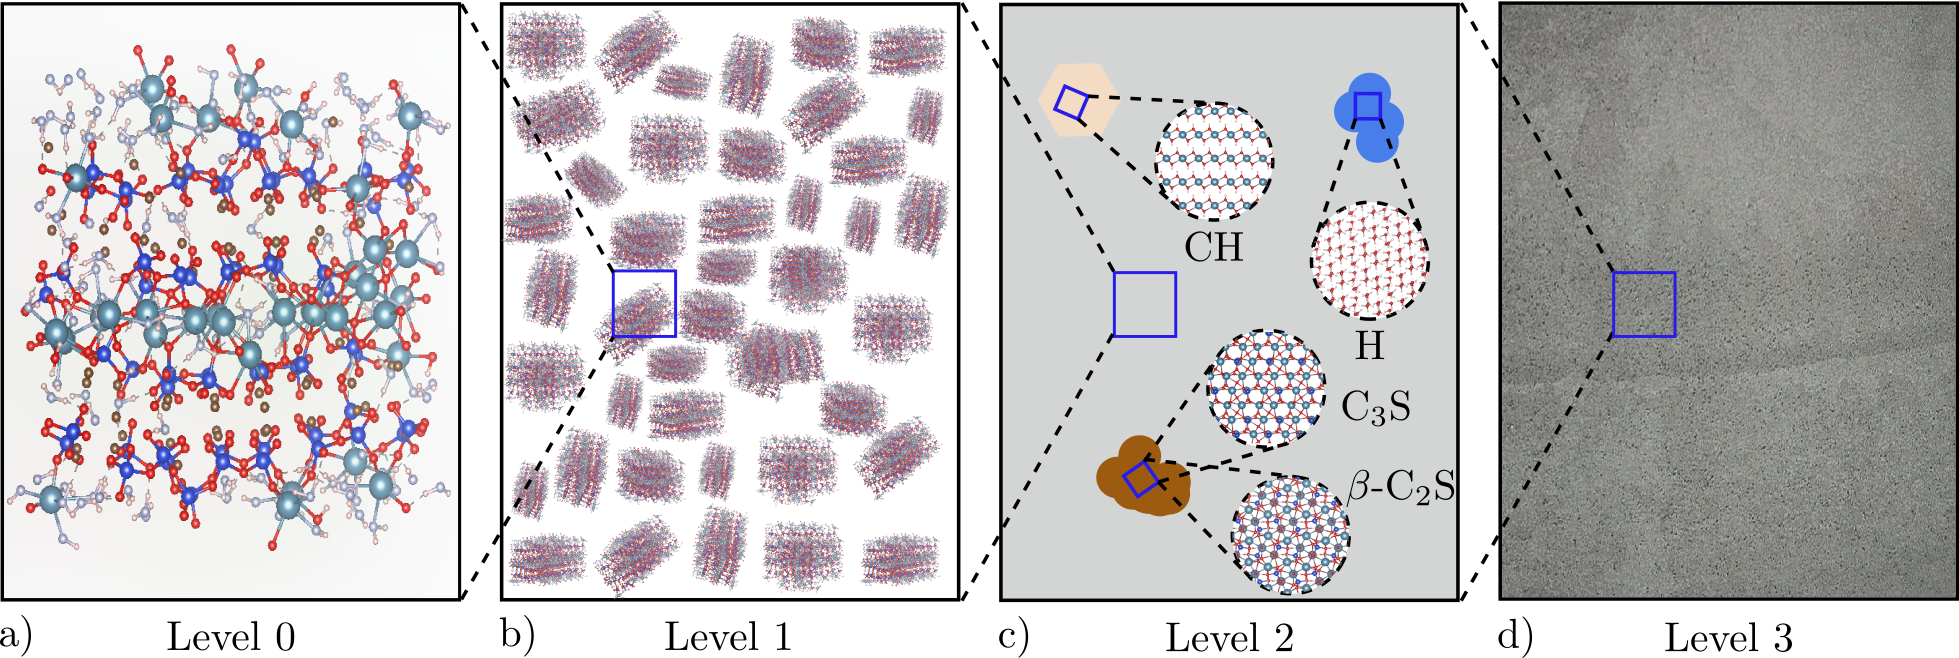
\includegraphics[width=0.8\textwidth]{levels.png}
    \caption{A four-level model representing the upscaling of C-S-H properties from the nanoscale to the engineering scale. (a) snapshot of C-S-H's nanostructure. (b) microstructure of C-S-H created by agglomeration of randomly oriented C-S-H nanoparticles. (c) microtexture of hardened paste composed by hydration products. (d) macrotexture of cement paste at the engineering scale. Adapted from \supercite{AbdolhosseiniQomi2015}.}
    \label{fig:figure1}
\end{figure}



% Chapter Template

\chapter{Theoretical Background} % Main chapter title

\label{Chapter2} % Change X to a consecutive number; for referencing this chapter elsewhere, use \ref{ChapterX}

\lhead{Chapter 2. \emph{Theoretical Background}}
This chapter is devoted to present the theoretical foundations and formalism of Density Functional Theory (DFT) and related methods required for the development of the results presented in this work. Starting with the many-body Schrödinger equation, this chapter covers the Born-Oppenheimer approximation, the Hartree-Fock approximation, Hohenberg-Kohn theorems, the Kohn-Sham equations, exchange-correlation functionals, and definitions on Ab initio molecular dynamics (AIMD) and machine learning force fields (MLFFs), along with implementation details in the Vienna Ab initio Simulation Package (VASP).

Ultimately, this chapter aims to provide a comprehensive understanding of the theoretical framework that underpins the computational methods utilised in this work, enabling the reader to grasp the principles and assumptions that govern the simulations and analyses performed throughout.

\section{Many Body Schrödinger Equation}
In the realm of materials science, comprehending particle behaviour within a system inevitably demands resorting to intricate principles of quantum mechanics. Our journey shall commence by describing the physical laws that shape the interactions among particles constituting a system---electrons and nuclei alike. 

\subsection{The Coulomb Interaction}

Materials may be thought of as complex assemblies of electrons and nuclei, held together by a delicate balance between attractive Coulomb interactions---primarily between electrons and nuclei---and repulsive interactions between like-charged particles, such as electron-electron and nucleus-nucleus pairs, which govern the overall dynamics of the material system\supercite{giustino2014materials, sholl2023density, kaxiras2003atomic}.  From classical electrostatics, these interactions can be mathematically expressed as follows: 

\begin{itemize}
\item Electron-electron interactions 
  \begin{equation}
    \label{eq1}
    \hat{V}_{ee} = \frac{1}{2} \sum_{i\neq j} \frac{e^2}{4\pi\epsilon_0 |\mathbf{r}_i - \mathbf{r}_j|}
  \end{equation}
\item Electron-nucleus interactions 
  \begin{equation}
    \label{eq2}
    \hat{V}_{nn} = \frac{1}{2} \sum_{I\neq J} \frac{e^2}{4\pi\epsilon_0} \frac{Z_I Z_J}{|\mathbf{R}_I - \mathbf{R}_J|}
  \end{equation}
\item Electron-nuclei interactions 
\begin{equation}
    \label{eq3}
    \hat{V}_{en} = -\sum_{i\neq I} \frac{e^2}{4\pi\epsilon_0} \frac{Z_I}{|\mathbf{r}_i - \mathbf{R}_I|}
  \end{equation}
\end{itemize}

where $e$ is the electronic charge, $\epsilon_0$ is the vacuum permittivity, $Z_I$ and $Z_J$ are the atomic numbers of nuclei $I$ and $J$, respectively, and $\mathbf{r}_i$ and $\mathbf{R}_I$ are the position vectors of electrons and nuclei, respectively. Moreover, we must also consider the kinetic energy of the collection of electrons and nuclei
\begin{equation}
    \label{eq4}
    \hat{T} = -\sum_i \frac{\hbar^2}{2m_e} \nabla_i^2 - \sum_I \frac{\hbar^2}{2M_I} \nabla_I^2
\end{equation}
where $\hbar$ is the reduced Planck's constant, $m_e$ is the electron mass, and $M_I$ is the mass of the nucleus $I$.

\subsection{The Time-Independent Schrödinger Equation}
The Time-Independent Schrödinger Equation (TISE) lies at the heart of non-relativistic quantum mechanics, providing a mathematical framework to describe stationary electronic states of quantum systems. It takes the following form:
\begin{equation}
  \label{eq5}
  \hat{H} \psi(\mathbf{r}) = E \psi(\mathbf{r})
\end{equation}
where $\hat{H}$ is the Hamiltonian of the system, encompassing both kinetic and potential energies, $\psi(\mathbf{r})$ is the wavefunction of the system, and $E$ is the energy eigenvalue associated with the state described by $\psi(\mathbf{r})$.  It is important to note that Equation \ref{eq5} is only applicable to a single particle, yet a material system is composed of many electrons (N) and nuclei (M) with spatial coordinates $\mathbf{r}_1, \mathbf{r}_2, \ldots, \mathbf{r}_N$ and $\mathbf{R}_1, \mathbf{R}_2, \ldots, \mathbf{R}_M$, respectively. Therefore, we must introduce a so-called many-body wavefunction given by:
\begin{equation}
  \Psi(\mathbf{r}_1, \mathbf{r}_2, \ldots, \mathbf{r}_N, \mathbf{R}_1, \mathbf{R}_2, \ldots, \mathbf{R}_M)
  \label{eq5b}
\end{equation}
On this basis, the many-body version of Equation \ref{eq5} shall be constructed by combining the kinetic (Equation \ref{eq4}) and potential (Equations \ref{eq1}, \ref{eq2}, and \ref{eq3}) energy contributions, leading to the following expression:
\begin{equation}
  \label{eq6}
  \begin{split}
    \left[
      -\sum_i \frac{\hbar^2}{2m_e} \nabla_i^2 
      - \sum_I \frac{\hbar^2}{2M_I} \nabla_I^2 
      + \frac{1}{2} \sum_{i\neq j} \frac{e^2}{4\pi\epsilon_0 |\mathbf{r}_i - \mathbf{r}_j|} +\right. \\
      \left. \frac{1}{2} \sum_{I\neq J} \frac{e^2}{4\pi\epsilon_0} \frac{Z_I Z_J}{|\mathbf{R}_I - \mathbf{R}_J|} 
      - \sum_{i, I} \frac{e^2}{4\pi\epsilon_0} \frac{Z_I}{|\mathbf{r}_i - \mathbf{R}_I|}
    \right]\Psi = E_{\text{tot}} \Psi
  \end{split}
\end{equation}
Equation \ref{eq6} provides a complete description of the stationary states of a non-relativistic many-body system, under time-independent conditions and in the absence of external fields. Additionally, we can achieve a more compact formulation by introducing the concept of atomic units. To this end, let us consider the simplest electron-nucleus system---the hydrogen atom---where the electron orbital has an average radius $a_0 \approx 0.529 \, \text{Å}$. Thereby, the Coulomb energy for such a system is given by:
\begin{equation}
  \label{eq7}
  E_{\text{Ha}} = \frac{e^2}{4 \pi \epsilon_0 a_0}
\end{equation}
where 'Ha' stands for Hartree. Within this framework, the Hartree energy represents the Coulomb interaction between two fundamental charges separated by a distance of one Bohr radius ($a_0$). Moreover, the angular momentum quantisation condition for the electron in the hydrogen atom is given by
\begin{equation}
  \label{eq8}
  m_e v a_0 = \hbar
\end{equation}
Additionally, the equilibrium condition between the nuclear attraction and the electron's centrifugal force can be expressed as:
\begin{equation}
  \label{eq9}
  \frac{e^2}{4 \pi \epsilon_0 a_0^2} = \frac{m_e v^2}{a_0}
\end{equation}
By combining Equations \ref{eq7}, \ref{eq8}, and \ref{eq9}, we derive the 
following relationships:
\begin{equation}
  \label{eq10}
  \frac{e^2}{4 \pi \epsilon_0 a_0} = \frac{\hbar^2}{m_e a_0^2}
\end{equation}
\begin{equation}
  \label{eq11}
  \frac{1}{2} m_e v^2 = \frac{1}{2}E_{\text{Ha}}
\end{equation}
This latter relation showcases that the kinetic energy is of the same order as $E_\text{Ha}$, rendering it convenient to normalise Equation \ref{eq6} by this quantity:
\begin{equation}
  \label{eq12}
  \begin{split}
    \left[
      -\sum_i \frac{1}{2}a_0^2 \nabla_i^2 
      - \sum_I \frac{1}{2} \frac{1}{(M_I/m_e)} \nabla_I^2 
      + \frac{1}{2} \sum_{i\neq j} \frac{a_0}{|\mathbf{r}_i - \mathbf{r}_j|}\right. \\
      \left. +  \frac{1}{2} \sum_{I\neq J} Z_I Z_J \frac{a_0}{|\mathbf{R}_I - \mathbf{R}_J|} 
      - \sum_{i, I} Z_I \frac{a_0}{|\mathbf{r}_i - \mathbf{R}_I|}
    \right]\Psi = \frac{E_{\text{tot}}}{E_{\text{Ha}}} \Psi
  \end{split}
\end{equation}
A final simplification involves setting our energy units to Ha, distance units to $a_0$, and mass units to $m_e$. The last missing constant $e$ is set to 1, leading to the following expression: 
\begin{equation}
  \label{eq13}
  \begin{split}
    \left[
      -\sum_i \frac{\nabla_i^2}{2}
      - \sum_I \frac{\nabla_I^2}{2 M_I} 
      + \frac{1}{2} \sum_{i\neq j} \frac{1}{|\mathbf{r}_i - \mathbf{r}_j|} + \right. \\
      \left. \frac{1}{2} \sum_{I\neq J} \frac{Z_I Z_J} {|\mathbf{R}_I - \mathbf{R}_J|} 
      - \sum_{i, I} \frac{Z_I}{|\mathbf{r}_i - \mathbf{R}_I|}
    \right]\Psi = E_{\text{tot}} \Psi
  \end{split}
\end{equation}

Ultimately, even though Equation \ref{eq13} provides an exact method capable of yielding various properties of a material system---such as elastic, thermal, and electronic properties---a combination of mathematical complexity and computational limitations renders it intractable to solve for any realistic system. Moreover, the wavefunction contains vastly more information than is necessary to describe most observable properties of a material. Therefore, we must resort to alternative formulations that allow us to extract only the relevant information from the wavefunction whilst reducing the computational cost of the calculations. The remainder of this chapter is dedicated to presenting such alternative approaches that ultimately lead to the computational methods employed throughout this work.

%-----------------------------------
%	SUBSECTION 1
%-----------------------------------
\section{The Born-Oppenheimer Approximation}
For atoms in a solid, we can think of nuclei as being held immobile in a fixed position, while electrons instantaneously react to any nucleus's movement. This assumption is based on the fact that nuclei are much heavier than electrons---by three to four orders of magnitude---making the former behave like classical particles. Thereby, we can rewrite the many-body wavefunction as a product of two wavefunctions:
\begin{equation}
  \Psi(\mathbf{r}_1, \mathbf{r}_2, \ldots, \mathbf{r}_N, \mathbf{R}_1, \mathbf{R}_2, \ldots, \mathbf{R}_M) = \psi_{\mathbf{R}}(\mathbf{r}_1, \mathbf{r}_2, \ldots, \mathbf{r}_N)\chi(\mathbf{R})
  \label{eq14}
\end{equation}
where $\psi_{\mathbf{R}}$ is the electronic wavefunction parametrised by the nuclear positions $\mathbf{R}$, and $\chi$ is the nuclear wavefunction. Furthermore, this significant mass disparity enables a systematic approximation scheme, in which the electronic wavefunction is solved for fixed nuclei, and its solution is used as an effective potential for the nuclear dynamics afterwards. First, nuclei' kinetic energy is neglected, as their positions are assumed to be fixed: 
\begin{equation}
  \label{eq15}
  \sum_I \frac{\nabla_I^2}{2 M_I} = 0
  \quad \text{and} \quad  E = E_{\text{tot}} - \sum_{I<J} \frac{Z_I Z_J}{|\mathbf{R}_I - \mathbf{R}_J|}
\end{equation}
Following, we define the Coulomb potential of the nuclei experienced by the electrons as:
\begin{equation}
  \label{eq16}
  V_{\text{n}}(\mathbf{r}) = - \sum_{I} \frac{Z_I}{|\mathbf{r} - \mathbf{R}_I|}
\end{equation}
Then, Equation \ref{eq13} can be rewritten as:
\begin{equation}
  \label{eq17}
  \left[
    -\sum_i \frac{\nabla_i^2}{2} + \sum_i V_{\text{n}}(\mathbf{r}_i) + \frac{1}{2} \sum_{i\neq j} \frac{1}{|\mathbf{r}_i - \mathbf{r}_j|} 
  \right] \Psi = E \Psi 
\end{equation}
Finally, by using Equation \ref{eq14}, we can define the electronic and nuclear Schrödinger equations as follows:
\begin{equation}
  \label{eq18}
  \left[
    -\sum_i \frac{\nabla_i^2}{2} + \sum_i V_{\text{n}}(\mathbf{r}_i) + \frac{1}{2} \sum_{i\neq j} \frac{1}{|\mathbf{r}_i - \mathbf{r}_j|} 
  \right] \psi_{\mathbf{R}} = E_{\mathbf{R}} \psi_{\mathbf{R}}
\end{equation}
\begin{equation}
  \label{eq19}
  \left[
    -\sum_I \frac{\nabla_I^2}{2 M_I} + \sum_{I<J} \frac{Z_I Z_J}{|\mathbf{R}_I - \mathbf{R}_J|} + E(\mathbf{R}_1,\dots,\mathbf{R}_M)\right] \chi(\mathbf{R}) = E_{\text{tot}} \chi(\mathbf{R})
\end{equation}
where $E_{\mathbf{R}}= E(\mathbf{R}_1,\dots,\mathbf{R}_M)$ is the electronic surface energy, which is a function of the nuclear positions, and serves as an effective potential shaping the nuclear dynamics. 

%-----------------------------------
%	SUBSECTION 2
%-----------------------------------

\section{Hartree-Fock Approximation}
The essence of the Hartree-Fock approximation (HFA) is to approximate the interacting many-electron system (Equation \ref{eq17}) by a set of non-interacting single-particle problems subject to an effective mean-field potential\supercite{martin2016interacting, helgaker2014molecular, feng2005introduction}. As a means to this, we first rewrite the total wavefunction for a system with N electrons as the product of single-electron wavefunctions---often referred to as the Hartree approximation\supercite{Hartree1928}---as showcased in Equation \ref{eq20}. 
\begin{equation}
  \Psi^H(\mathbf{r}_1, \dots, \mathbf{r}_N) = \prod_{i=1}^N \phi_i(\mathbf{r}_i)
  \label{eq20}
\end{equation}
Following, we construct the total energy functional as the expectation value of the Hamiltonian operator:
\begin{equation}
  \label{eq21}
\begin{aligned}
  E^{H}[\{\phi_i\}] &= \bigg\langle \Psi^H \bigg| \hat{H} \bigg| \Psi^H \bigg\rangle 
\end{aligned}
\end{equation}
Expanding Equation \ref{eq21}:
\begin{equation}
  \label{eq22}
  \begin{split}
    E^{H}[\{\phi_i\}] &= \sum^N_{i=1} \int \phi_i^*(\mathbf{r}) \left(-\frac{\nabla^2}{2} + V_{\text{n}}(\mathbf{r})\right) \phi_i(\mathbf{r}) d\mathbf{r}  + \frac{1}{2} \sum_{i\neq j} \int\int \frac{|\phi_i(\mathbf{r})|^2 |\phi_j(\mathbf{r'})|^2 }{|\mathbf{r} - \mathbf{r'}|} d\mathbf{r} d\mathbf{r'}
  \end{split}
\end{equation}
where the first term adds up the kinetic energy and electron-nuclear attraction overall electrons, whilst the second accounts for the classical electron-electron repulsion energy averaged over the electron density distribution. In order to find the set of orbitals $\{\phi_i\}$ that minimises the total energy functional, we use the variational principle where we shall impose the orthonormality condition: 
\begin{equation}
  \label{eq23}
  \int \phi_i^*(\mathbf{r}) \phi_j(\mathbf{r}) d\mathbf{r} = \delta_{ij}
\end{equation}
for what we introduce the Lagrange multipliers $\lambda_{ij}$ to enforce these constraints and define the Lagrangian:
\begin{equation}
  \label{eq24}
  \mathcal{L} = E^H[\{\phi_i\}] - \sum_{i=1}^{N}\lambda_{ij} ( \langle\phi_i|\phi_j\rangle - \delta_{ij})
\end{equation}
which ultimately simplifies to:
\begin{equation}
  \label{eq25}
  \mathcal{L} = E^H[\{\phi_i\}] - \sum_{i=1}^{N}\varepsilon_{i} ( \langle\phi_i|\phi_i\rangle - 1)
\end{equation}

Then, we need to compute the derivative of $\mathcal{L}$ with respect to $\phi_i^*$ and set it to zero:
\begin{equation}
  \label{eq26}
  \frac{\delta \mathcal{L}}{\delta \phi_i^*}(\mathbf{r}) = 0
\end{equation}
which yields to the Hartree equation:
\begin{equation}
  \label{eq27}
  \left[-\frac{\nabla^2}{2} + V_{\text{n}}(\mathbf{r}) + V^H_i(\mathbf{r})\right]\phi_i(\mathbf{r})  = \varepsilon_i \phi_i(\mathbf{r})
\end{equation}
where $V_n(\mathbf{r})$ represents the electrostatic interaction between electrons and nuclei, and the Hartree potential 
\begin{equation}
  \label{eq28}
  V^H_i(\mathbf{r}) = \sum_{j\neq i} \int \frac{|\phi_j(\mathbf{r'})|^2}{|\mathbf{r} - \mathbf{r'}|} d\mathbf{r'}
\end{equation}
accounts for the average electrostatic interaction experienced by the $i$-th electron due to all other electrons in the system. This effective mean-field potential replaces the electron-electron interactions, effectively simplifying the many-body problem into single-particle problems. 
\subsection{The Pauli Exclusion Principle}
So far, we have introduced the Hartree approximation, which assumes that the many-electron wavefunction can be expressed as a product of single-particle wavefunctions. However, this approach does not account for the indistinguishability of electrons and the Pauli exclusion principle, which states that no two fermions--- half-spin particles, such as electrons---can reside in the same quantum state simultaneously. In doing so, it imposes a restriction on the possible configurations of electrons in a system that shall be accounted for.
 
 In order to achieve this, V. Fock\supercite{Fock1930} introduced a different approximation to the wavefunction by using a Slater determinant---a mathematical construct that combines one-electron wavefunctions in such a way that satisfies the antisymmetry principle. This is done by expressing the overall wavefunction as the determinant of a matrix of single-electron wavefunctions:
\begin{equation}
  \Psi^{HF}(\mathbf{r}_1, \dots, \mathbf{r}_N) = \frac{1}{\sqrt{N!}} \begin{vmatrix}
    \phi_1(\mathbf{r}_1) & \phi_1(\mathbf{r}_2) & \dots & \phi_1(\mathbf{r}_N)\\
    \phi_2(\mathbf{r}_1) & \phi_2(\mathbf{r}_2) & \dots & \phi_2(\mathbf{r}_N)\\
    \vdots & \vdots & \ddots & \vdots\\
    \phi_N(\mathbf{r}_1) & \phi_N(\mathbf{r}_2) & \dots & \phi_N(\mathbf{r}_N)
  \end{vmatrix}
  \label{eq29}
\end{equation}
where $1/\sqrt{N!}$ is a normalisation factor. To illustrate this, consider a two-electron system with single-particle wavefunctions $\phi_1(\mathbf{r})$ and $\phi_2(\mathbf{r})$. The Slater determinant for this system would be:
\begin{equation}
  \Psi^{HF}(\mathbf{r}_1, \mathbf{r}_2) = \frac{1}{\sqrt{2}} \begin{vmatrix}
    \phi_1(\mathbf{r}_1) & \phi_1(\mathbf{r}_2)\\
    \phi_2(\mathbf{r}_1) & \phi_2(\mathbf{r}_2)
  \end{vmatrix} = \frac{1}{\sqrt{2}} \left[\phi_1(\mathbf{r}_1)\phi_2(\mathbf{r}_2) - \phi_1(\mathbf{r}_2)\phi_2(\mathbf{r}_1))\right]
  \label{eq30}
\end{equation}
Evidently, $\Psi^{HF}(\mathbf{r}_1, \mathbf{r}_2) = -\Psi^{HF}(\mathbf{r}_2, \mathbf{r}_1)$, which satisfies the antisymmetr principle. 
\subsection{The Hartree-Fock Equations}
The Hartree-Fock equations are derived in a similar manner we addressed the Hartree equations. We first define the total energy with the Hartree-Fock wavefunction (Equation \ref{eq29}) 
\begin{equation}
  \label{eq31}
  \begin{split}
    E^{HF}[\{\phi_i\}] &= \bigg\langle \Psi^{HF} \bigg| \hat{H} \bigg| \Psi^{HF} \bigg\rangle\\
    &= \sum_{i} \langle \phi_i \big|\frac{\nabla^2}{2} + V_{\text{n}}(\mathbf{r})\big| \phi_i \rangle\\
    &+ \frac{1}{2} \sum_{i\neq j} \langle \phi_i \phi_j \big| \frac{1}{|\mathbf{r}_i - \mathbf{r}_j|} \big| \phi_i \phi_j\rangle\\
    &- \frac{1}{2} \sum_{i\neq j} \langle \phi_i \phi_j \big| \frac{1}{|\mathbf{r}_i - \mathbf{r}_j|} \big| \phi_j \phi_i\rangle
  \end{split}
\end{equation}
Consequently, using the variational principle, we derive the Hartree-Fock equations: 
\begin{equation}
  \label{eq32}
  \left[-\frac{\nabla^2}{2} + V_{\text{n}}(\mathbf{r}) + V^H_i(\mathbf{r}) +\right]\phi_i(\mathbf{r})
  - \sum_{j\neq i} \langle \phi_j \big| \frac{1}{|\mathbf{r}_i - \mathbf{r}_j|} \big| \phi_i \rangle \phi_j(\mathbf{r})
  = \varepsilon_i \phi_i(\mathbf{r})
\end{equation}
Noticeably, Equation \ref{eq32} has an extra term compared with the Hartree equation (Equation \ref{eq27}). This term is called the "exchange" term\supercite{kaxiras2003atomic}, and describes the effects of exchange between electrons. It is convenient to try to express the Hartree-Fock equations in a more compact form, so we define the single-particle and total densities as 
\begin{equation}
  \label{eq33}
  \rho_i(\mathbf{r}) = |\phi_i(\mathbf{r})|^2
\end{equation}
\begin{equation}
  \label{eq34}
  \rho(\mathbf{r}) = \sum_i \rho_i(\mathbf{r}) 
\end{equation}
so the Hartree potential can be expressed as 
\begin{equation}
  \label{eq35}
  V^H_i(\mathbf{r}) = \sum_{j\neq i}  \int \frac{\rho_j(\mathbf{r'})}{|\mathbf{r} - \mathbf{r'}|} d\mathbf{r'} 
  = \int \frac{\rho(\mathbf{r'}) - \rho_i(\mathbf{r'})}{|\mathbf{r} - \mathbf{r'}|} d\mathbf{r'}
\end{equation}
Therefore, the single-particle exchange density can be constructed as 
\begin{equation}
  \label{eq36}
  \rho^X_i(\mathbf{r}, \mathbf{r'}) = \sum_{j\neq i}\frac{\phi_i(\mathbf{r'})\phi^*_i(\mathbf{r})\phi_j(\mathbf{r})\phi^*_j(\mathbf{r'})}{\phi_i(\mathbf{r})\phi^*_i(\mathbf{r})}
\end{equation}
Finally, the Hartree-Fock equations take the form 
\begin{equation}
  \label{eq37}
  \left[-\frac{\nabla^2}{2} + V_{\text{n}}(\mathbf{r}) + V^H_i(\mathbf{r}) + V^X_i(\mathbf{r})\right]\phi_i(\mathbf{r}) = \varepsilon_i \phi_i(\mathbf{r})
\end{equation}
where $V^X_i$ stands for the exchange potential
\begin{equation}
  \label{eq38}
  V^X_i(\mathbf{r}) = -\int \frac{\rho^X_i(\mathbf{r}, \mathbf{r'})}{|\mathbf{r} - \mathbf{r'}|} d\mathbf{r'}
\end{equation}

%----------------------------------------------------------------------------------------
%	SECTION 2
%----------------------------------------------------------------------------------------
\section{Density Functional Theory}
So far, we have acknowledged that determining the state of a system with N electrons remains a formidable challenge, for it involves a wavefunction defined in a $3N$-dimensional space. We also recognise that it is possible---heuristically speaking---to simplify such representation by utilising products of single-particle wavefunctions. Nevertheless, such independent electrons approximation necessitates the wavefunctions to be explicitly specified, thereby yielding a rather drastic approximation for the behaviour of the system. Thus, it is natural to consider a different approach to develop the appropriate single-particle framework in an exact manner, onto which approximations can be introduced afterwards.

We hereby introduce the Density Functional Theory (DFT), which draws upon the insight that any property of a system of many electrons can be viewed as a functional of the ground-state density $n(\mathbf{r})$\supercite{martin2020electronic} (Equation \ref{eq39})---a scalar function defined over three spatial coordinates. 
\begin{equation}
  n(\mathbf{r}) = N \int \Psi^*(\mathbf{r}, \ldots, \mathbf{r}_N) \Psi(\mathbf{r},\ldots, \mathbf{r}_N) d\mathbf{r}_2 \ldots d\mathbf{r}_N
  \label{eq39}
\end{equation}
The foundational principles of DFT were established in the original papers by Hohenberg, Kohn and Sham\supercite{Hohenberg1964, Kohn1965}, where they present two theorems that establish the theoretical framework of DFT.
However, for the purposes of this discussion, we shall base our exposition on explanatory texts\supercite{martin2020electronic, giustino2014materials, kaxiras2003atomic, sholl2023density}.


\subsection{First Hohenberg-Kohn Theorem}

\begin{theorem}[First Hohenberg-Kohn Theorem]
  The ground-state electron density $n(\mathbf{r})$ uniquely determines the external potential $V(\mathbf{r})$ and, consequently, the ground-state energy $E_0$ of a many-electron system.
\end{theorem}
\begin{proof}
  Suppose two different external potentials, $V(\mathbf{r})$ and $V'(\mathbf{r})$ (different ionic potentials) yield the same ground-state electron density $n(\mathbf{r})$. Given that $V(\mathbf{r})$ and $V'(\mathbf{r})$ are different in a non-trivial way, we will show that this statement leads to a contradiction. Let $E$ and $\Psi$ be the total energy and wavefunction and $E'$ and $\Psi'$ be the total energy and wavefunction corresponding to the systems with hamiltonians $\hat{H}$ and $\hat{H}'$, respectively, with the first hamiltonian containing $V(\mathbf{r})$  and the second containing $V'(\mathbf{r})$ as an external potential:
  \begin{equation*}
    \hat{H} = \hat{T} + \hat{U} + V, \quad \hat{H}' = \hat{T} + \hat{U} + V', \quad E = \langle \Psi | \hat{H} | \Psi \rangle, \quad E' = \langle \Psi' | \hat{H}' | \Psi' \rangle 
  \end{equation*}
  Here, $\hat{T}$ and $\hat{U}$ correspond to the kinetic and interaction energy operators, thereby being common for both hamiltonians. Now, we assume that the ground states of the two hamiltonians are different because the external potentials are different. Then, according to the variational principle: 
  \begin{equation}
    \label{eq40}
    \begin{aligned}
      E < \langle \Psi'|\hat{H}|\Psi'\rangle &= \langle \Psi'|\hat{T} + \hat{U} + V + V' - V' |\Psi'\rangle \\
      &= \langle \Psi'|\hat{H}' + V - V' |\Psi'\rangle \\
      &= E' + \langle \Psi'|(V - V')|\Psi'\rangle
    \end{aligned}
  \end{equation}
  Following the same reasoning, we can prove that 
  \begin{equation}
    \label{eq41}
    E' < E - \langle \Psi|(V - V')|\Psi\rangle
  \end{equation}
  Adding Equations \ref{eq40} and \ref{eq41}, we obtain:
  \begin{equation}
    \label{eq42}
    E + E' < E' + E - \langle \Psi|(V - V')|\Psi\rangle + \langle \Psi'|(V - V')|\Psi'\rangle
  \end{equation}
  where the last two terms result in 
  \begin{equation}
    \label{eq43}
    \int n'(\mathbf{r}) (V - V') d\mathbf{r} - \int n(\mathbf{r}) (V - V') d\mathbf{r} = 0
  \end{equation}
  since $n(\mathbf{r})=n'(\mathbf{r})$ by assumption. Finally, we arrive at the following expression: 
  \begin{equation}
    \label{eq44}
    E + E' < E + E'
  \end{equation}
  Evidently, this is a contradiction, which implies that our initial assumption about the densities being the same ought to be false, thereby proving there is a one-to-one correspondence between an external potential $V(\mathbf{r})$ and the electron density $n(\mathbf{r})$. Moreover, since $V(\mathbf{r})$ determines the wavefunction, the wavefunction must be a unique functional of the density. So we conclude that the expression  
  \begin{equation}
    \label{eq45}
    \mathcal{F}[n(\mathbf{r})] = \langle \Psi |\hat{T} + \hat{U} |\Psi \rangle 
  \end{equation}
  must be a universal functional of the electronic density---\emph{i.e.}, common to all solids---and that the ground state energy is a functional of the density: 
  \begin{equation}
    \label{eq46}
    E[n(\mathbf{r})] = \mathcal{F}[n(\mathbf{r})] + \int V(\mathbf{r}) n(\mathbf{r}) d\mathbf{r}
  \end{equation}
\end{proof}

\subsection{Second Hohenberg-Kohn Theorem}
\begin{theorem}[Second Hohenberg-Kohn Theorem]
  The ground-state energy $E$ can be obtained through the variation of trial densities $\tilde{n}(\mathbf{r})$ instead of trial wavefunctions $\tilde{\Psi}$.
\end{theorem}
\begin{proof}
  First, we fix a trial density $\tilde{n}(\mathbf{r})$ and define the trial wavefunctions $\tilde{\Psi}^{\alpha}_{\tilde{n}(\mathbf{r})}$. Therefore, the constrained energy minimum is defined as 
\begin{equation}
  \label{eq47}
  \begin{aligned}
    E[\tilde{n}(\mathbf{r})] &= \min_{\alpha} \langle \tilde{\Psi}^{\alpha}_{\tilde{n}(\mathbf{r})} | \hat{H} | \tilde{\Psi}^{\alpha}_{\tilde{n}(\mathbf{r})} \rangle\\
    &= \mathcal{F}[\tilde{n}(\mathbf{r})] + \int V(\mathbf{r}) \tilde{n}(\mathbf{r}) d\mathbf{r}
  \end{aligned}
\end{equation}
  Secondly, we minimise Equation \ref{eq47} over all $n$
  \begin{equation}
    \label{eq48}
    E = \min_{\tilde{n}(\mathbf{r})} E[\tilde{n}(\mathbf{r})] = \min_{\tilde{n}(\mathbf{r})} \left\{\mathcal{F}[\tilde{n}(\mathbf{r})] + \int V(\mathbf{r}) \tilde{n}(\mathbf{r}) d\mathbf{r}\right\}
  \end{equation}
For a non-degenerate ground state, the minimum corresponds to the ground-state $n(\mathbf{r})$, or to one of the ground-state densities otherwise.
\end{proof}
Finally, we have managed to map the formidable challenge of finding the minimum of $\langle \Psi | \hat{H} | \Psi \rangle$ involving a $3N$-dimensional wavefunction into a much simpler problem of finding the minimum of $E[n(\mathbf{r})]$ involving a $3$-dimensional function. This is the essence of DFT, which allows us to compute the ground-state properties of many-electron systems without explicitly solving the many-body Schrödinger equation.

\subsection{Kohn-Sham Equations}
Even though the Hohenberg-Kohn theorems provide a rigorous foundation for DFT, they offer no guidance whatsoever for constructing the functional $\mathcal{F}[n(\mathbf{r})]$. As such, density functional theory would lack practical utility if it were not for the auxiliary system proposed by Kohn and Sham\supercite{martin2020electronic}. It consists of replacing the many-electron problem by an auxiliary independent-particle problem that yields the same ground-state density, incorporating the many-body effects into a so-called exchange-correlation functional. To this end, we first define the density of the auxiliary system as
\begin{equation}
  n(\mathbf{r}) = \sum_i |\phi_i(\mathbf{r})|^2
  \label{eq49}
\end{equation}
where $\phi_i(\mathbf{r})$ are the single-particle wavefunctions of the auxiliary system. Next, we define the independent-particle kinetic energy functional as 
\begin{equation}
  \label{eq50}
  T_s[n(\mathbf{r})] = \frac{1}{2}\sum_i \int \phi_i^*(\mathbf{r}) (-\nabla^2 )\phi_i(\mathbf{r}) d\mathbf{r}
\end{equation}
and the Hartree energy functional can be redefined as 
\begin{equation}
  \label{eq51}
  E_H[n(\mathbf{r})] = \frac{1}{2} \int \frac{n(\mathbf{r}) n(\mathbf{r'})}{|\mathbf{r} - \mathbf{r'}|} d\mathbf{r} d\mathbf{r'}
\end{equation}
yielding the following expression for the total energy functional:
\begin{equation}
  \label{eq52}
  E[n(\mathbf{r})] = T_s[n(\mathbf{r})] + \int V_{\text{n}}(\mathbf{r}) n(\mathbf{r}) d\mathbf{r} + E_H[n(\mathbf{r})] + E_{xc}[n(\mathbf{r})]
\end{equation}
where $E_{xc}[n(\mathbf{r})]$ is the exchange-correlation energy functional is defined as
\begin{equation}
  \label{eq53}
  E_{xc}[n(\mathbf{r})] = \langle \hat{T} \rangle - T_s[n(\mathbf{r})] + \langle \hat{U}\rangle - E_H[n(\mathbf{r})]
\end{equation}
having $\langle \hat{T} \rangle$ and $\langle \hat{U} \rangle$ being the exact kinetic energy and electron-electron interaction energy. Finally, we choose a variation in the density to be 
\begin{equation}
  \delta n(\mathbf{r}) = \delta \phi_i^*(\mathbf{r}) \phi_i(\mathbf{r}) 
  \label{eq54}
\end{equation}
along with the following constraint 
\begin{equation}
  \int \delta n(\mathbf{r}) d\mathbf{r} = \int \delta \phi_i^*(\mathbf{r}) \phi_i(\mathbf{r}) d\mathbf{r} = 0
  \label{eq55}
\end{equation}
and by applying the Kohn-Sham variational principle, we arrive at the Kohn-Sham equations: 
\begin{equation}
  \label{eq56}
  \left[-\frac{\nabla^2}{2} + V_{\text{ext}}(\mathbf{r}) + V_H(\mathbf{r}) + V_{xc}(\mathbf{r})\right]\phi_i(\mathbf{r}) = \varepsilon_i \phi_i(\mathbf{r})
\end{equation}
where $V_{\text{ext}}(\mathbf{r})$ is the external potential, $V_H(\mathbf{r})$ is the Hartree potential, and $V_{xc}(\mathbf{r})$ is the exchange-correlation potential defined as 
\begin{equation}
  \label{eq57}
  V_{xc}(\mathbf{r}) = \frac{\delta E_{xc}[n(\mathbf{r})]}{\delta n(\mathbf{r})}
\end{equation}
Our task now shall focus on constructing appropriate approximations for the exchange-correlation functional $E_{xc}[n(\mathbf{r})]$. 

\subsection{Exchange-Correlation Functionals}
The usefulness of DFT relies entirely on whether reliable approximations for the exchange-correlation functional $E_{xc}[n(\mathbf{r})]$ can be constructed with sufficient accuracy and computational efficiency. Therefore, we shall now present the most commonly used approximations for $E_{xc}[n(\mathbf{r})]$, as well as their strengths and weaknesses.  
\subsubsection{Local Density Approximation}
The simplest---and remarkably effective---approximation for the exchange-correlation functional is the local-density approximation (LDA)\supercite{Kohn1999}. It approximates the exchange-correlation energy of an inhomogeneous electron system by that of a homogeneous electron gas (HEG) having the same electron density. 
\begin{equation}
  \label{eq58}
  E_{xc}^{LDA}[n(\mathbf{r})] = \int n(\mathbf{r}) \epsilon_{xc}(n(\mathbf{r})) d\mathbf{r}
\end{equation}
where $\epsilon_{xc}(n)$  is the exchange and correlation energy per electron of a uniform electron gas of density $n$\supercite{Hohenberg1964, Kohn1965}. This quantity depends solely on the local density and surrounding electrons in the vicinity of $\mathbf{r}$, for example, a sphere of radius $\sim\lambda_F(\mathbf{r})$---the local Fermi wavelength\supercite{feng2005introduction} $\lambda_F(\mathbf{r})\equiv[3\pi^2 n(\mathbf{r})]^{-1/3}$.

The exchange and correlation contributions to $E_{xc}^{LDA}$ can be separated into two terms 
\begin{equation}
  \label{eq59}
  E_{xc}^{LDA}[n(\mathbf{r})] = E_x^{HEG}[n(\mathbf{r})] + E_c^{HEG}[n(\mathbf{r})]
\end{equation}
The first term corresponds to the exchange energy density contribution
\begin{equation}
  \label{eq60}
  \begin{aligned}
    \epsilon_x^{HEG}(n) &= -\frac{3}{4} \left(\frac{3}{\pi}\right)^{1/3} n^{1/3}\\
    %&= -\frac{3 \lambda_F}{4\pi} \\
    &= -\frac{0.458128}{r_s}
  \end{aligned}
\end{equation}
where $r_s$ is the Wigner-Seitz radius---the radius of a sphere containing one electron and given by $(4\pi/3)r_s^3 = n^{-1}$.

The second term corresponds to the correlation energy, which was computed by Ceperley and Alder\supercite{Ceperley1980} using quantum Monte Carlo methods. Subsequently, the extracted data was parameterised by Perdew and Zunger\supercite{Perdew1981}, yielding the following expression:
\begin{equation}
  \label{eq61}
  \epsilon_c^{HEG}(r_s) = \begin{cases} 
    0.0311\ln{r_s} - 0.0480 + 0.002 r_s \ln{r_s} - 0.0116 r_s& r_s < 1\\
   \displaystyle \frac{-0.1423}{1 + 1.0529\sqrt{r_s} + 0.3334 r_s}& r_s \geq 1
  \end{cases}
\end{equation}
LDA has demonstrated remarkable success for most applications involving systems with slowly varying densities or systems with high densities. Nevertheless, LDA---and its spin-polarised version (LSDA)---
breaks down in systems governed by strong correlation effects that it loses any resemblance to non-interacting electron gases.   

\subsubsection{Generalised Gradient Approximation}
In contrast to LDA---which considers the electronic density to be locally uniform---the generalised gradient approximation (GGA) systematically improves upon LDA by incorporating not only the local density $n(\mathbf{r})$, but also its gradient $\nabla n(\mathbf{r})$, thereby accounting for the inhomogeneities in the electron distribution.  

Within this framework, the exchange-correlation energy functional is expressed as a function of the local density and its gradient 
\begin{equation}
  \label{eq62}
  E_{xc}^{GGA}[n(\mathbf{r})] = \int n(\mathbf{r}) \epsilon_{xc}^{HEG}(n(\mathbf{r})) f(n_{\uparrow}(\mathbf{r}), n_{\downarrow}(\mathbf{r}),\nabla n_{\uparrow}(\mathbf{r}), \nabla n_{\downarrow}(\mathbf{r})) d\mathbf{r}
\end{equation}
where $n_{\uparrow}(\mathbf{r})$ and $n_{\downarrow}(\mathbf{r})$ are the spin-up and spin-down electron densities, respectively. Additionally, the exact form of $f$---a parametrised analytic function---depends on the GGA under consideration.  

In this regard, one of the most prominent and widely adopted GGA functionals is the Perdew-Burke-Ernzerhof (PBE)\supercite{Perdew1996} functional, which was proposed as a solution for the drawbacks of previously proposed GGAs, such as the Perdew-Wang (PW91) functional. Within PBE, all parameters---other than those in $\epsilon_{xc}^{HEG}(n(\mathbf{r}))$---are fundamental constants. Consequently, the exchange energy term in the PBE functional is given by 
\begin{equation}
  \label{eq63}
  E_{x}^{PBE} = \int n(\mathbf{r}) \epsilon_{x}^{HEG}(n(\mathbf{r})) \left[1 + \kappa - \frac{\kappa}{1 +  \mu s^2/\kappa}\right] d\mathbf{r}
\end{equation}
where $\kappa = 0.804$ and $\mu = 0.219$ are the parameters of the PBE functional, $k_F = (3\pi^2 n(\mathbf{r}))^{1/3}$ is the local Fermi wavevector and $s = |\nabla n(\mathbf{r})|/(2k_F n(\mathbf{r}))$ is a dimensionless density gradient.

The correlation energy term in the PBE functional is expressed as 
\begin{equation}
  \label{eq64}
  E_{c}^{PBE} = \int n(\mathbf{r}) \left[\epsilon_{c}^{HEG} + 
  \gamma \phi^3 \ln\left\{ 1 + \frac{\beta}{\gamma}t^2 
  \left[ 
  \frac{1 + At^2}{1 + At^2 + A^2t^4}
  \right]
  \right\} 
  \right]
\end{equation}
where $\gamma = 0.031091$, $\beta = 0.066725$, $\phi$ is a spin-scaling factor, and $A$ and $t$ are defined as 
\begin{equation}
  \label{eq65}
  A = \frac{\beta}{\gamma} \left[\exp{\frac{-\epsilon_{c}^{HEG}}{\gamma\phi^3}} - 1  \right]^{-1}, \quad 
  t(\mathbf{r}) = \frac{|\nabla n(\mathbf{r})|}{2\phi k_s n(\mathbf{r})}
\end{equation}
where $k_s = \sqrt{4 k_F / \pi}$ is the Thomas-Fermi screening wavenumber.

Even though PBE holds a significant advantage over LDA in terms of accuracy, it is not exempt from certain limitations and shortcomings.  PBE tends to overestimate equilibrium lattice constants by about 1\%---LDA underestimates them by the same amount---which is detrimental for accurate calculations of other equilibrium properties, such as bulk moduli, phonon frequencies and magnetism.

To address this issue, a revised version of the PBE---the PBEsol functional\supercite{Perdew2008}---was developed, which improves equilibrium properties of densely-packed solids and their surfaces, reducing the overestimation of lattice constants by a factor of $\sim 4$. Nonetheless, PBEsol does not perform well for semiconductors and can lead to less accurate total energy calculations compared to PBE.  Ultimately, the choice of GGA functional comes down to the specific system and properties under investigation, as well as the desired balance between accuracy and computational efficiency.

\subsubsection{Hybrid Functionals}
Aforementioned functionals and their inherent limitations motivated the exploration of hybrid functionals. They offer improved accuracy by incorporating a fraction of the exact nonlocal Hartree-Fock exchange energy into the exchange-correlation functional, allowing efficient yet accurate calculations. 

One of these functionals includes PBE0\supercite{Heyd2003}---a combination of the PBE functional and the exact Hartree-Fock exchange energy. It is defined as 
\begin{equation}
  \label{eq66}
  E_{xc}^{PBE0} = \frac{1}{4}E_{x}^{HF} + \frac{3}{4}E_{x}^{PBE} + E_{c}^{PBE}
\end{equation}
Another prominent example is the HSE (Heyd-Scuseria-Ernzerhof) functional\supercite{Moussa2012}, which splits the exchange energy into short-range (SR) and long-range (LR) contributions
\begin{equation}
  \label{eq67}
  E_{xc}^{HSE06} = \frac{1}{4}E_{x}^{HF,SR}(\omega) + \frac{3}{4}E_{x}^{PBE,SR}(\omega) + E_{c}^{PBE,LR}(\omega) + E_{c}^{PBE}(\omega)
  \end{equation}
  where $\omega$ is an adjustable parameter that controls the short and long-range separation in the decomposed Coulomb operator
  \begin{equation}
    \label{eq68}
    \frac{1}{r} = SR_{\omega}(\mathbf{r}) + LR_{\omega}(\mathbf{r}) = 
    \frac{erfc(\omega r)}{r} + \frac{erf(\omega r)}{r}
  \end{equation}
  While hybrid functionals often surpass LDA and GGA in terms of accuracy, they come at a higher computational cost, rendering them less suitable for large-scale calculations.  
  
\section{Ab initio Molecular Dynamics}

\subsection{Born-Oppenheimer Molecular Dynamics}

\subsection{Car-Parrinello Molecular Dynamics}

\section{Machine Learning Force Fields}
\subsection{Hyperparameters}

\section{Computational Implementation in VASP}
\subsection{Plane Wave Basis Set}
\subsection{K-Point Sampling and Cutoff Energy}
\subsection{Pseudopotentials}
\section{Density of States}




%%----------------------------------------------------------------------------------------

% Chapter 3

\chapter{Methodology} % Main chapter title

\label{Chapter3} % For referencing the chapter elsewhere, use \ref{Chapter1} 

\lhead{Chapter 3. \emph{Methodology}} % This is for the header on each page - perhaps a shortened title



The computational investigations are conducted using the Vienna Ab initio Simulation Package (VASP). The crystal structures analyzed conform to the general formula XGeTe$_{3}$, which includes three specific compounds:  

\begin{itemize}  
	\item CrGeTe$_{3}$, characterized by a chromium electronic configuration of \([Ar]: 3d^5 4s^1\),  
	\item MnGeTe$_{3}$, with a manganese electronic configuration of \([Ar]: 3d^6 4s^2\), and  
	\item FeGeTe$_{3}$, exhibiting an iron electronic configuration of \([Ar]: 3d^7 4s^2\).  
\end{itemize}  

Each crystal structure is defined by a unit cell containing 10 atoms, corresponding to two formula units (f.u.) per unit cell. The common elements in these structures, germanium (Ge) and tellurium (Te), have electronic configurations of \([Ar]: 4s^2 4p^2\) and \([Ar]: 5s^2 5p^4\), respectively. Additionally, these structures share identical symmetry characteristics, corresponding to space group 147.  

The electronic properties are analyzed using Projector Augmented Wave (PAW) potentials. The ab initio study begins with spin-polarized calculations on the CrGeTe$_{3}$ monolayer, which are subsequently extended to the MnGeTe$_{3}$ and FeGeTe$_{3}$ monolayers. The Perdew-Burke-Ernzerhof (PBE) functional is initially employed. Since the ground state of each monolayer may involve magnetic configurations (either ferromagnetic or antiferromagnetic), we systematically determine the appropriate cutoff energy and k-point mesh for each structure.  

A suitable energy cutoff for all three monolayers is established, adhering to the convergence criterion outlined in Section \ref{cutoff-energy}. A plane-wave basis with a cutoff energy of 500 eV is applied, meeting a convergence criterion of less than 1 meV/f.u., achieved through a Monkhorst-Pack mesh. We optimize the k-point mesh by performing several ionic position optimizations to derive the optimal lattice parameters, as discussed in the Two-Dimensional Equation of State (Section \ref{2D.eqs}). A convergence criterion of 1 m\AA. is adopted, leading to the selection of a \(10 \times 10 \times 1\) k-point grid.  

The calculations incorporate a self-consistency loop break condition of \(1 \times 10^{-6}\) eV to minimize undesired Pulay stress and ensure an adequate plane-wave basis set. This two-step convergence criterion ensures accurate description of any XGeTe$_{3}$ crystal structure, regardless of the magnetic phase. Following the determination of these parameters, we perform ionic position optimizations to obtain the ground states for both the ferromagnetic and antiferromagnetic phases, ultimately identifying the more stable magnetic configuration for each monolayer.  

Subsequent calculations utilize the PBEsol functional to assess potential improvements in electronic properties compared to existing experimental and theoretical studies of the monolayers. To account for the strong correlation among \(d\) electrons in each monolayer, Hubbard \(U\) corrections are applied using both PBE and PBEsol functionals, which modify the magnetic moments of the transition metals and the potential band gaps, aligning closely with experimental and theoretical values. Full optimization calculations are conducted to evaluate the preservation of symmetry in the monolayers, facilitated by FINDSYM utility \supercite{stokes2005findsym}.  

Phonon calculations are performed using a \(3 \times 3 \times 1\) supercell for the stable magnetic phase of CrGeTe$_{3}$, and a \(4 \times 4 \times 1\) supercell for both MnGeTe$_{3}$ and FeGeTe$_{3}$. The vibrational properties of these structures are studied via the “atomic force from finite displacements” method implemented in the Phonopy package \supercite{phonopy-phono3py-JPCM,phonopy-phono3py-JPSJ}. The functional that most accurately describes each monolayer, based on previous analysis, is utilized for these calculations.  

Finally, we investigate ferromagnetic random alloys at three different concentrations: \(x = 0.25\), \(x = 0.50\), and \(x = 0.75\). These random alloys take the forms Cr\(_{x}\)GeMn\(_{1-x}\)Te\(_{3}\), Cr\(_{x}\)GeFe\(_{1-x}\)Te\(_{3}\), and Fe\(_{x}\)GeMn\(_{1-x}\)Te\(_{3}\), each containing 24 formula units (f.u.). The alloys are generated using the mcsqs code \supercite{atat5}, which implements a Monte Carlo algorithm to find the best special quasi-random structure. This code is part of the Alloy-Theoretic Automated Toolkit (ATAT) \supercite{atat1,atat2,atat3,atat4,atat5,atat6,atat7,atat8,atat9,atat10,atat11,atat12,atat13,atat14,atat15,atat16}. Subsequently, VASP is employed for electronic optimizations, utilizing only the PBE functional. 
\section{Flow of VASP}

\begin{itemize}
	\item VASP selects the appropriate pseudopotential method for the calculation, using the Projector-Augmented Wave (PAW) method. This method ensures a precise treatment of core electrons while maintaining computational efficiency. Additionally, VASP employs an exchange-correlation functional as specified by the user.
	\item The initial electronic density is computed.
	\item VASP iteratively constructs the Kohn-Sham Hamiltonian in a self-consistent (SC) manner.
	\item The electronic density is updated at each iteration, and the effective potential is recalculated until the self-consistent cycle converges to a predefined tolerance level. This tolerance, typically set by the user, is recommended to be $1 \times 10^{-6}$ eV, as suggested in the VASP documentation \supercite{EDIFF}. See Fig. \ref{fig:cycle_scf}.
\end{itemize}

\begin{figure}[H]
	\includegraphics[width=14cm]{Figures/cycle_scf.jpg}
	\centering
	\caption{Flowchart adapted from the works of Gross\supercite{Gross2003} and Barhoumi\supercite{barhoumi2021}, illustrating the self-consistent field (SCF) cycle in density functional theory (DFT) calculations, as implemented in VASP. The cycle starts with an initial guess for the electron density $n^{0}(\mathbf{r})$, followed by the construction of the effective potential $v^{j}_{\text{eff}}(\mathbf{r})$, incorporating the Hartree potential, exchange-correlation functional, and pseudopotentials. The Kohn-Sham equations are then solved to obtain updated wavefunctions, which are used to recalculate the electron density. This iterative process continues until the difference between successive effective potentials falls below a predefined tolerance, typically $1 \times 10^{-6}$ eV \supercite{EDIFF}. The cycle ensures convergence to the ground-state electronic structure \supercite{Kohn1965,blochl1994}.}
	\label{fig:cycle_scf}
\end{figure}
\section{VASP Input and Output Files}

This section provides a detailed explanation of the required input files for VASP calculations and the output files generated during the process.

\subsection{Input Files}
To perform a VASP calculation, four essential input files are required: INCAR, POSCAR, KPOINTS, and POTCAR.

\subsubsection{INCAR}
The INCAR file contains the parameters that govern various aspects of the calculation in VASP. Each parameter influences different stages of the simulation, such as electronic structure optimization, Density of States (DOS) calculations, ionic relaxation, and magnetization settings.

\begin{figure}[H]  
	\centering  
	\begin{threeparttable}  
		\caption{Example of an INCAR file used for optimizing ionic positions while keeping the cell size and shape fixed. This file provides the total energy of the system. By applying it to different unit cell sizes, the Two-Dimensional Equation of State \ref{2D.eqs} can be used to determine the optimal lattice parameters. For further details, refer to the VASP manual.}
		\label{fig:fig3.1}  
		\resizebox{\textwidth}{!}{  
			\begin{tabular}{>{\columncolor{blue!10}}l>{\columncolor{blue!10}}l>{\columncolor{blue!10}}l>{\columncolor{blue!10}}l>{\columncolor{blue!10}}l>{\columncolor{blue!10}}l>{\columncolor{blue!10}}l>{\columncolor{blue!10}}l>{\columncolor{blue!10}}l>{\columncolor{blue!10}}l>{\columncolor{blue!10}}l>{\columncolor{blue!10}}l>{\columncolor{blue!10}}l>{\columncolor{blue!10}}l>{\columncolor{blue!10}}l>{\columncolor{blue!10}}l>{\columncolor{blue!10}}l>{\columncolor{blue!10}}l>{\columncolor{blue!10}}l}  
				\hline   
				\multicolumn{3}{c}{\cellcolor{blue!10} \textbf{GENERAL}}& & & & & & & & & & & & & & & &\\   
				\textbf{SYSTEM} & \textbf{= XGeTe$_3$} & \textit{\# System name defined by the user}& & & & & & & & & & & & & & & & \\   
				\textbf{PREC}   & \textbf{= Accurate} & & & & & & & & & & & & & & & & &\\
				\multicolumn{3}{c}{\cellcolor{blue!10} \textbf{ELECTRONIC OPTIMIZATION}} & & & & & & & & & & & & & & & &\\   
				\textbf{ENCUT}  & \textbf{= 500}  & \textit{\# Cutoff energy (in eV)}& & & & & & & & & & & & & & & & \\   
				\textbf{LREAL}  & \textbf{= Auto} & & & & & & & & & & & & & & & & &\\
				\textbf{ISMEAR} & \textbf{= 0}    & \textit{\# -5 for insulators, 1 or 2 for metals} & & & & & & & & & & & & & & & &\\   
				\textbf{ALGO}   & \textbf{= Normal} & & & & & & & & & & & & & & & & &\\
				\multicolumn{3}{c}{\cellcolor{blue!10} \textbf{DOS CALCULATION}}& & & & & & & & & & & & & & & & \\   
				\textbf{LORBIT} & \textbf{= 11}  & \textit{\# Necessary for DOS calculations}& & & & & & & & & & & & & & & &\\   
				\textbf{NEDOS}  & \textbf{= 4000} & \textit{\# Number of DOS points}& & & & & & & & & & & & & & & &\\   
				\multicolumn{3}{c}{\cellcolor{blue!10} \textbf{IONIC RELAXATION}} & & & & & & & & & & & & & & & &\\   
				\textbf{ISIF}   & \textbf{= 2}   & \textit{\# Optimize ionic positions only \tnote{a}}& & & & & & & & & & & & & & & & \\   
				\textbf{IBRION} & \textbf{= 2}   & \textit{\# Conjugate gradient algorithm}& & & & & & & & & & & & & & & &\\   
				\textbf{EDIFF}  & \textbf{= 1E-06} & \textit{\# Energy convergence criterion} & & & & & & & & & & & & & & & &\\   
				\textbf{NELM}   & \textbf{= 100} & \textit{\# Maximum number of SCF iterations} & & & & & & & & & & & & & & & &\\   
				\textbf{NSW}    & \textbf{= 100} & \textit{\# Maximum number of ionic steps}& & & & & & & & & & & & & & & &\\   
				\multicolumn{3}{c}{\cellcolor{blue!10} \textbf{MAGNETIZATION}}& & & & & & & & & & & & & & & &\\   
				\textbf{ISPIN}  & \textbf{= 2}   & \textit{\# Spin-polarized calculation}& & & & & & & & & & & & & & & &\\   
				\textbf{MAGMOM} & \textbf{= 2*3 2*0 6*0} & \textit{\# Initial magnetic moments \tnote{b}} & & & & & & & & & & & & & & & &\\   
				\hline  
			\end{tabular}  
		}  
		\begin{tablenotes}  
			\footnotesize  
\begin{minipage}{\textwidth}
	\item[a] By default ISIF$=3$ optimizes ionic positions, cell shape, and cell volume. For monolayers, cell size relaxation is typically restricted to the x and y directions. To achieve this, modifications are made to the default 'vasp\_std' script to perform the desired two-dimensional cell size optimization.
	\item[b] Magnetic moments are assigned according to the atom order in the POSCAR and POTCAR files. In this example: 2 atoms of X $\times$ $\mu_B$(X), 2 atoms of Ge $\times$ $\mu_B$(Ge), and 6 atoms of Te $\times$ $\mu_B$(Te).
\end{minipage}
		\end{tablenotes}  
	\end{threeparttable}  
\end{figure}

Proper definition of the tags in the INCAR file is essential. Incorrect or unnecessary tag usage can lead to unrealistic results. Therefore, it is crucial to be meticulous and always refer to the official VASP manual for guidance.
 

\subsubsection{POSCAR}
The POSCAR file serves as a comprehensive blueprint for defining the atomic structure of materials and molecules in computational simulations. It consists of several key sections, each containing specific information essential for accurate simulations. The first line is often a comment for human readability, providing a brief description of the system without affecting the calculation. Following this, the lattice vectors are provided, which define the shape and size of the unit cell. These vectors can be specified either in Cartesian or fractional coordinates, as illustrated in Figure \ref{fig:fig3.2}.
\begin{figure}[H]
\resizebox{\textwidth}{!}{
	\begin{tabular}{>{\columncolor{blue!10}}c>{\columncolor{blue!10}}c>{\columncolor{blue!10}}c>{\columncolor{blue!10}}l>{\columncolor{blue!10}}l>{\columncolor{blue!10}}l>{\columncolor{blue!10}}l>{\columncolor{blue!10}}l>{\columncolor{blue!10}}l>{\columncolor{blue!10}}l>{\columncolor{blue!10}}l>{\columncolor{blue!10}}l>{\columncolor{blue!10}}l>{\columncolor{blue!10}}l>{\columncolor{blue!10}}>{\columncolor{blue!10}}l>{\columncolor{blue!10}}l>{\columncolor{blue!10}}l>{\columncolor{blue!10}}l>{\columncolor{blue!10}}l>{\columncolor{blue!10}}l>{\columncolor{blue!10}}l>{\columncolor{blue!10}}l>{\columncolor{blue!10}}l>{\columncolor{blue!10}}l>{\columncolor{blue!10}}l}\hline
		\multicolumn{3}{l}{\cellcolor{blue!10} \textbf{ X Ge Te}} & & & & & & & & & & & & & & & & & & & & & &\\
		\multicolumn{3}{l}{\cellcolor{blue!10}1.0}& & & & & & & & & & & & & & & & & & & & & &\\
		6.9068061733 & 0.0000000000 & 0.0000000000 & & & & & & & & & & & & & & & & & & & & & &\\
		-3.4534030866 & 5.9814696051 & 0.0000000000& & & & & & & & & & & &  & & & & & & & & & &\\
		0.0000000000 & 0.0000000000 & 21.8184108734 & & & & & & & & & & & & & & & & & & & & & &\\
		\multicolumn{3}{l}{\cellcolor{blue!10} \textbf{ X Ge Te }}& & & & & & & & & & & && & & & & & & & & & \\
		\multicolumn{3}{l}{\cellcolor{blue!10} 2   2   6}& & & & & & & & & & & & & & & & & & & & & &\\
		\multicolumn{3}{l}{\cellcolor{blue!10}Direct} & & & & & & & & & & & & & & & & & & & & & &\\
		0.666666687 & 0.333333343 & 0.500000000 & & & & & & & & & & & & & & & & & & & & & &\\
		0.333333343 & 0.666666687 & 0.500000000 & & & & & & & & & & & & & & & & & & & & & &\\
		0.000000000 & 0.000000000 & 0.444593012& & & & & & & & & & & & & & & & & & & & & &\\
		0.000642670 & 0.373393325 & 0.421062350& & & & & & & & & & & & & & & & & & & & & &\\
		0.999357343 & 0.626606705 & 0.578937650 & & & & & & & & & & & & & & & & & & & & & &\\
		0.626606705 & 0.627303362 & 0.421062350& & & & & & & & & & & & & & & & & & & & & &\\
		0.373393325 & 0.372696668 & 0.578937650& & & & & & & & & & & & & & & & & & & & & &\\
		0.372696668 & 0.999357343 & 0.421062350 & & & & & & & & & & & & & & & & & & & & & &\\
		0.627303362 & 0.000642670 & 0.578937650& & & & & & & & & & & & & & & & & & & & & &\\ \hline
	\end{tabular}
 }
	\centering
	\caption{Unit cell structure in fractional coordinates for the XGeTe$_3$ (X = Cr, Mn, Fe) monolayer, containing 10 atoms: 2 X atoms, 2 Ge atoms, and 6 Te atoms.}
	\label{fig:fig3.2}
	\label{poscar}
\end{figure}

A scaling factor, typically provided after the lattice vectors, allows for resizing the simulation cell without altering the atomic coordinates. The file then specifies the atomic species present in the system and their corresponding quantities, whether they are standard elements or user-defined labels.

In essence, the POSCAR file provides comprehensive input for computational simulations, ensuring an accurate representation of the atomic structure within the system. For further details, refer to the official VASP manual\supercite{POSCAR}.
\subsubsection{KPOINTS}
The KPOINTS file provides essential instructions for defining the sampling of the Brillouin zone, which is a fundamental region in reciprocal space related to the periodic structure of a crystal. The choice of k-points significantly affects the accuracy of the calculations by determining how the wavefunctions are sampled in this region.
\begin{figure}[H]
\resizebox{\textwidth}{!}{
	\begin{tabular}{>{\columncolor{blue!10}}c>{\columncolor{blue!10}}l>{\columncolor{blue!10}}l>{\columncolor{blue!10}}l>{\columncolor{blue!10}}l>{\columncolor{blue!10}}l>{\columncolor{blue!10}}l>{\columncolor{blue!10}}l>{\columncolor{blue!10}}l>{\columncolor{blue!10}}l>{\columncolor{blue!10}}l>{\columncolor{blue!10}}l>{\columncolor{blue!10}}l>{\columncolor{blue!10}}l>{\columncolor{blue!10}}l>{\columncolor{blue!10}}l>{\columncolor{blue!10}}l>{\columncolor{blue!10}}l>{\columncolor{blue!10}}l>{\columncolor{blue!10}}l>{\columncolor{blue!10}}l>{\columncolor{blue!10}}l>{\columncolor{blue!10}}l>{\columncolor{blue!10}}l>{\columncolor{blue!10}}l>{\columncolor{blue!10}}l>{\columncolor{blue!10}}l>{\columncolor{blue!10}}l>{\columncolor{blue!10}}l>{\columncolor{blue!10}}l>{\columncolor{blue!10}}l>{\columncolor{blue!10}}l>{\columncolor{blue!10}}l>{\columncolor{blue!10}}l>{\columncolor{blue!10}}l>{\columncolor{blue!10}}l>{\columncolor{blue!10}}l} \hline
		\multicolumn{1}{l}{\cellcolor{blue!10} \textbf{k-points}} & & & & & & & & & & & & & & & & & & & & & & & & & & & & & & & & & & & &\\ 
		\multicolumn{1}{l}{\cellcolor{blue!10}0}& & & & & & & & & & & & & & & & & & & & & & & & & & & & & & & & & & & &\\
		\multicolumn{1}{l}{\cellcolor{blue!10} \textbf{Gamma}}& & & & & & & & & & & & & & & & & & & & & & & & & & & & & & & & & & & &\\ 
		6 6 1& & & & & & & & & & & & & & & & & & & & & & & & & & & & & & & & & & & & \\
		0 0 0& & & & & & & & & & & & & & & & & & & & & & & & & & & & & & & & & & & & \\  \hline
	\end{tabular}
 }
	\centering
	\caption{K-point grid centered at the Gamma point in the Brillouin zone. The dimensions "6 6 1" define the grid in the x, y, and z directions, respectively. The value "1" in the z direction indicates a 2D system, such as a monolayer.}
	\label{fig:fig3.3}
	\label{kpoints}
\end{figure}
Different schemes can be employed to select k-points. One commonly used method is the Monkhorst-Pack scheme, which ensures a uniform distribution of points across the Brillouin zone. The Brillouin zone is constructed from the reciprocal lattice and represents a Wigner-Seitz cell, characterized by paths that pass through high-symmetry points. For the systems under study, this path is $\Gamma$-$M$-$K$-$\Gamma$. See Fig. \ref{fig:brillouin_zone} for a top view of the Brillouin zone and the corresponding high-symmetry points.

\begin{figure}[H]
	\centering
	\includegraphics[width=10cm]{Figures/brillouin_zone.png}
	\caption{Top view of the Brillouin zone of XGeTe$_{3}$ monolayers, showing the path through the high-symmetry points that define its Wigner-Seitz unit cell.}
	\label{fig:brillouin_zone}
\end{figure}

Alternatively, Gamma-centered grids can be used, as shown in Figure \ref{fig:fig3.3}, where the k-points are centered at the Gamma point of the Brillouin zone. The automatic generation of k-points is also an option depending on the complexity and symmetry of the system under study.

Each k-point can be assigned a weight, indicating its relative contribution to the total energy and other physical properties calculated. Proper weighting of k-points is crucial for achieving accurate and efficient results. For additional details, please refer to the official VASP manual\supercite{KPOINTS}.
\subsubsection{POTCAR}
The POTCAR file acts as a specialized instruction manual for computers during computational simulations. It aids the computer in comprehending the behavior of atoms within materials. Within this manual, default settings dictate the computer's calculations. These settings encompass various aspects, including the selection of exchange-correlation functionals, and the utilization of simplified atom models such as PAW.

These details are meticulously chosen based on both theoretical principles and experimental observations to ensure that the computer's predictions closely align with real-world phenomena. Recognizing the significance of the POTCAR file cannot be overstated. It serves as the bedrock for the computer's operations. By adhering to the appropriate settings and rules outlined in the POTCAR file, the computer can generate highly accurate predictions regarding the behavior of materials.

\subsection{Output files}
Upon completing ab initio calculations, several output files provide crucial information about the simulation results. These files offer insights into the electronic structure, energy convergence, atomic positions, and other important parameters. Here are brief descriptions of some of the most important output files:

\subsubsection{OUTCAR}
The \texttt{OUTCAR} file is a comprehensive output log that contains detailed information from the electronic structure calculations. This includes convergence criteria, energy values, forces acting on atoms, magnetic moments, and electronic band structure data. It serves as a valuable source for analyzing the simulation results in depth.

\subsubsection{CONTCAR}
The \texttt{CONTCAR} file contains the final atomic coordinates after the relaxation or optimization process. It is essential for visualizing the relaxed atomic structure and can be used as an input for subsequent calculations, ensuring continuity between simulations.

\subsubsection{DOSCAR}
The \texttt{DOSCAR} file provides information about the density of states (DOS), which represents the distribution of electronic states across a specified energy range. This file is essential for analyzing the electronic properties of a system and understanding its behavior under various conditions. One significant feature of this file is that it allows the calculation of the number of valence electrons, \( N_v \), which characterize the system under study. The number of valence electrons can be computed using the following equation:

\begin{equation}
	N_v = \int_{-\infty}^{\varepsilon_{F}} n(\varepsilon) \, d\varepsilon 
\end{equation}

Here, \( n(\varepsilon) \) is the density of states as a function of energy \( \varepsilon \), and \( \varepsilon_{F} \) is the Fermi energy. This integration is performed over the energy states up to the Fermi level.

\subsubsection{PROCAR}
The \texttt{PROCAR} file contains data about the projected electronic band structure, revealing the contributions of each atomic orbital to the electronic states. This information is indispensable for analyzing the electronic structure and the orbital character of the material.

\subsubsection{OSZICAR}
The \texttt{OSZICAR} file records the convergence behavior of both the electronic and ionic iterations during the calculation. It provides details on the energy convergence and the progress of the optimization, which is important for assessing the reliability and accuracy of the simulation results.

\section{Phonon calculations using Phonopy software}

The process of phonon calculation begins with a full relaxation of the atomic structure, where all degrees of freedom are optimized until the forces on each atom converge to a stable configuration. This optimization step generates a \texttt{CONTCAR} file, which contains the final equilibrium positions of atoms. Subsequently, supercells are constructed, where atoms are displaced to simulate the vibrational modes of the material. The displacements are calculated using Phonopy with the following command:

\begin{figure}[H]
	\begin{tabular}{>{\columncolor{black}}p{\linewidth}}
		\texttt{\textcolor{green!70!black}{username:\textcolor{blue}{$\sim$}}\textcolor{white}{\$} \textcolor{white}{phonopy -d --dim="2 2 1" --magmom="3 3 0 0 0 0 0 0 0 0"}} \\ \hline
	\end{tabular}
	\centering
	\caption{Creation of displacements for a supercell: The command \texttt{phonopy -d --dim} generates the displaced structures required for force calculations. The \texttt{--magmom} tag is essential when dealing with magnetic atoms.}
	\label{fig:fig3.4}
	\label{displacements}
\end{figure}

The underlying theory behind lattice vibrations is essential for understanding the thermodynamic, mechanical, and vibrational properties of crystalline solids. In a crystal, each atom oscillates around its equilibrium position, giving rise to vibrational modes, or phonons, which can either be acoustic or optical. As detailed by \textit{Kittel}\supercite{kittel2021} and \textit{Ashcroft}\supercite{ashcroft1976}, these modes are crucial for explaining key properties such as heat capacity, thermal conductivity, and electron-phonon interactions.

The nuclear positions in a crystal lattice are described as:
\begin{equation}
	\mathbf{R}_I(t) = \mathbf{R}_l + \mathbf{u}_I(t),
\end{equation}
where \( \mathbf{u}_I(t) \) represents the small displacement from equilibrium, and \( \mathbf{R}_l \) refers to the lattice points in the crystal. These displacements are often modeled within the harmonic approximation. According to Newton's second law, the equation of motion for these displacements is:
\begin{equation}
	M_I \ddot{\mathbf{u}}_I(t) = -\frac{\partial U}{\partial \mathbf{u}_I(t)},
\end{equation}
where \( M_I \) denotes the mass of the nucleus, and \( U \) represents the total potential energy of the system. In equilibrium, \( \frac{\partial U}{\partial \mathbf{u}_I} = 0 \), indicating that the system is stable. The potential energy \( U \) is expanded as a Taylor series around the equilibrium positions, and its second-order terms describe the harmonic interactions between neighboring atoms through the Born-von Karman force constants:
\begin{equation}
	K_{ls\alpha, l's'\beta} = \frac{\partial^2 U}{\partial (R_{l\alpha} + \tau_{s\alpha}) \partial (R_{l'\beta} + \tau_{s'\beta})}.
\end{equation}

From here, the equation of motion for the small displacements \( u_{I\alpha}(t) \) is reduced to:
\begin{equation}
	M_I \ddot{u}_{I\alpha}(t) = - \sum_{J\beta} \Phi_{I\alpha, J\beta} u_{J\beta}(t),
\end{equation}
where \( \Phi_{I\alpha, J\beta} \) are the force constants. These force constants are central to constructing the dynamical matrix, defined as:
\begin{equation}\label{eq:3.3}
	D_{s\alpha, s'\beta}(\mathbf{q}) = \frac{1}{(M_s M_{s'})^{1/2}} \sum_{l} e^{i\mathbf{q} \cdot \mathbf{R}_l} e^{i\mathbf{q} \cdot (\tau_{s'} - \tau_s)} K_{0s\alpha, ls'\beta},
\end{equation}
where \( D_{s\alpha, s'\beta}(\mathbf{q}) \) represents the dynamical matrix with the phonon wavevector \( \mathbf{q} \). Diagonalizing this matrix yields eigenvalues, corresponding to the square of the phonon frequencies \( \omega^2 \), and eigenvectors that represent the vibrational eigenmodes.  The eigenvalues distinguish between acoustic phonons, which are characterized by long-wavelength, in-phase oscillations of atoms, and optical phonons, where neighboring atoms oscillate out of phase. For a more in-depth analysis, see Chapter 7 of \textit{Giustino}'s book\supercite{Giustino2014}.

After generating the displaced supercells using Phonopy, VASP is employed to compute the forces acting on atoms in each supercell, as is indicated in Eq. \ref{eq:3.3}. This is achieved through single-point calculations, where the \texttt{INCAR} file is configured with specific tags tailored to this task, see Fig. \ref{incar_pho}. These calculations provide the force data necessary for constructing the force constants matrix \( \Phi \), which is crucial for determining the phonon frequencies and related vibrational properties.

\begin{figure}[H]
\resizebox{\textwidth}{!}{
\begin{tabular}{>{\columncolor{blue!10}}l>{\columncolor{blue!10}}l>{\columncolor{blue!10}}l>{\columncolor{blue!10}}l>{\columncolor{blue!10}}l>{\columncolor{blue!10}}l>{\columncolor{blue!10}}l>{\columncolor{blue!10}}l>{\columncolor{blue!10}}l>{\columncolor{blue!10}}l>{\columncolor{blue!10}}l>{\columncolor{blue!10}}l>{\columncolor{blue!10}}l>{\columncolor{blue!10}}l>{\columncolor{blue!10}}l>{\columncolor{blue!10}}l>{\columncolor{blue!10}}l>{\columncolor{blue!10}}l>{\columncolor{blue!10}}l>{\columncolor{blue!10}}l>{\columncolor{blue!10}}l>{\columncolor{blue!10}}l>{\columncolor{blue!10}}l>{\columncolor{blue!10}}l>{\columncolor{blue!10}}l>{\columncolor{blue!10}}l>{\columncolor{blue!10}}l}\hline
	\multicolumn{3}{c}{\cellcolor{blue!10} \textbf{GENERAL}} & & & & & & & & & & & & & & & & & & & & & & & &\\ 
	\textbf{SYSTEM} & = phonon calculation & & & & & & & & & & & & & & & & & & & & & & & & &\\ 
	\textbf{PREC}   & = Normal  &   & & & & & & & & & & & & & & & & & & & & & & & &\\ 
	\textbf{ISTART}   & = 0   &  & & & & & & & & & & & & & & & & & & & & & & & &\\ 
	\textbf{ICHARG}   & = 2  &   & & & & & & & & & & & & & & & &  & & & & & & & & \\ 
	\multicolumn{3}{c}{\cellcolor{blue!10} }& & & & & & & & & & & & & & & & & & & & & & & & \\ 
	\textbf{ENCUT}   & = 500   & & & & & & & & & & & & & & & & &  & & & & & & & &\\
	\textbf{SIGMA}   & = 0.05  & & & & & & & & & & & & & & & & & & & & & & & & &\\ 
	\textbf{ALGO}   & = Normal  & & & & & & & & & & & & & & & & & & & & & & & & &\\ 
	\textbf{LREAL}   & = .FALSE. &  & & & & & & & & & & & & & & & &  & & & & & & & &\\ 
	\textbf{EDIFF}   & = 1E-07   & & & & & & & & & & & & & & & & &  & & & & & & & &\\ 
	\textbf{NELM}   & = 100   &  & & & & & & & & & & & & & & & & & & & & & & & &\\ 
	\multicolumn{3}{c}{\cellcolor{blue!10} \textbf{OPTIMIZATION}}& & & & & & & & & & & & & & & &  & & & & & & & &\\ 
	\textbf{NSW} & = 0  & & & & & & & & & & & & & & & & &  & & & & & & & & \\ 
	\textbf{ISIF} & = 2 & & & & & & & & & & & & & & & & &  & & & & & & & & \\ 
	\multicolumn{3}{c}{\cellcolor{blue!10}} & & & & & & & & & & & & & & & &  & & & & & & & &\\ 
	\textbf{POTM} & = 0.5    & & & & & & & & & & & & & & & & &  & & & & & & & &\\
	\textbf{ISMEAR} & = 0    &  & & & & & & & & & & & & & & & & & & & & & & & &\\ 
	\textbf{IBRION} & = -1    & & & & & & & & & & & & & & & & & & & & & & & & &\\ 
	\textbf{LORBIT} & = 11   &  & & & & & & & & & & & & & & & & & & & & & & & &\\ 
	\multicolumn{3}{c}{\cellcolor{blue!10}} & & & & & & & & & & & & & & & & & & & & & & & &\\ 
	\textbf{ISPIN}   & = 2   &   & & & & & & & & & & & & & & & & & & & & & & & & \\ 
	\textbf{MAGMOM}  & = 8*3 8*0 24*0 &   & & & & & & & & & & & & & & & &  & & & & & & & &\\ 
	\multicolumn{3}{c}{\cellcolor{blue!10}} & & & & & & & & & & & & & & & & & & & & & & & &\\
	\textbf{LWAVE}   & = .FALSE. & & & & & & & & & & & & & & & & &  & & & & & & & &\\ 
	\textbf{ADDGRID}    & = .TRUE. & & & & & & & & & & & & & & & & &  & & & & & & & &\\ \hline
\end{tabular}
}
\centering
\caption{Configuration of the \texttt{INCAR} file for single-point calculations. Note the use of the \texttt{IBRION=-1} tag for this purpose. The magnetic order is specified by the \texttt{MAGMOM} tag, which must be consistent with the displacements generated in Fig. \ref{displacements}.}
\label{fig:fig3.5}
\label{incar_pho}
\end{figure}

To compute the forces from the VASP output file \texttt{vasprun.xml}, the following Phonopy command is used:

\begin{figure}[H]  
	\begin{tabular}{>{\columncolor{black}}p{\linewidth}}  
		\texttt{\textcolor{green!70!black}{username:\textcolor{blue}{$\sim$}}\textcolor{white}{\$} \textcolor{white}{phonopy -f pho\_POSCAR\{01..10\}/vasprun.xml}} \\ \hline  
	\end{tabular}  
	\centering  
	\caption{Command to compute force sets for each displaced supercell.}  
	\label{fig:fig3.6}  
	\label{forces}  
\end{figure}  

The computed forces are then used to derive key phonon properties, such as phonon dispersion curves (phonon bands) and the phonon density of states (DOS). These properties are calculated using Phonopy with the following commands:

\begin{figure}[H]  
	\resizebox{\textwidth}{!}{  
		\begin{minipage}[l]{\textwidth}  
			\subcaption{}  
			\centering  
			\begin{tabular}{>{\columncolor{blue!10}}l>{\columncolor{blue!10}}l>{\columncolor{blue!10}}l>{\columncolor{blue!10}}l>{\columncolor{blue!10}}l}\hline   
				\multicolumn{5}{l}{\cellcolor{black!100} \texttt{\textcolor{green!70!black}{username:\textcolor{blue}{$\sim$}}\textcolor{white}{\$} \textcolor{white}{phonopy -p -s band.conf}}} \\   
				\multicolumn{5}{c}{\cellcolor{white!10} } \\ \hline   
				\textbf{ATOM-NAME} & = Cr Ge Te & & &\\   
				\textbf{EIGENVECTORS}   & = .TRUE.  &  & &  \\   
				\textbf{DIM}   & = 2 2 1   &  & & \\   
				\textbf{BAND}   & = 0 0 0 & 0.5 0 0   &  0.333 0.33 0 & 0 0 0 \\   
				\textbf{BAND-POINTS}   & = 1001   & & &  \\   
				\textbf{BAND-LABELS}   & = $\Gamma$  M K $\Gamma$ &  & &\\  \hline  
			\end{tabular}  
			
			% Note below the table  
			\footnotesize \textit{Note: The high symmetry points ($\Gamma$, M, K) are indicative of the zone boundaries in the Brillouin zone and were obstained using the python module SeeK-path}.  
		\end{minipage}  
	}  
	\hfill  
	\resizebox{\textwidth}{!}{  
		\begin{minipage}[l]{\textwidth}  
			\subcaption{}  
			\centering  
			\begin{tabular}{>{\columncolor{blue!10}}l>{\columncolor{blue!10}}l>{\columncolor{blue!10}}l}\hline   
				\multicolumn{3}{l}{\cellcolor{black!100} \texttt{\textcolor{green!70!black}{username:\textcolor{blue}{$\sim$}}\textcolor{white}{\$} \textcolor{white}{phonopy -p -s dos.conf}}} \\   
				\multicolumn{3}{c}{\cellcolor{white!10} } \\ \hline  
				\textbf{DIM} & = 3 3 1 & \\   
				\textbf{MP}   & = 51 51 51   &   \\   
				\textbf{DOS}   & = .TRUE.   &  \\   
				\textbf{GAMMA-CENTER}   & = .TRUE.&  \\   
				\textbf{FPITCH}   & = 0.02  &  \\ \hline  
			\end{tabular}  
		\end{minipage}  
	}  
	\centering  
	\caption{Commands used to obtain (a) phonon band structure based on high-symmetry points provided by the SeeK-path tool \supercite{Hinuma2017,Togo2018}, and (b) phonon density of states (DOS).}  
	\label{pho_dos_bands}  
\end{figure}



\section{Implementation for generate random magnetic alloys: ATAT}

The theoretical background of this software package was discussed in Section \ref{sqs}. Here, we outline the input files required to generate quasi-random structures. Specifically, we employ the Monte Carlo approach (mcsqs method), which requires two input files: `rndstr.in` and `sqscell.out`.

The first file, `rndstr.in` (see Fig. \ref{fig:3.8} $\mathbf{a}$), is similar to the POSCAR file. It contains the lattice vectors and atomic positions of the system in its unit cell form, but also allows for partial occupations of atomic positions. The second file, `sqscell.out` (see Fig. \ref{fig:3.8} $\mathbf{b}$), specifies the supercell required to generate a Special Quasirandom Structure (SQS) that matches the desired compositions of the random alloy. 

For example, we cannot use a $3\times3\times1$ supercell for a desired composition of $x=0.25$ in a disordered (Cr,Mn) sublattice of the unit cell $Cr_{x}Mn_{1-x}GeTe_{3}$, since the smallest step in that supercell would be $1/3^2 = 1/9$. Therefore, the allowed concentrations for this supercell would be: 
$x=0, 1/9, 2/9, 1/3, 4/9, 5/9, 2/3, 7/9, 8/9, 1.$ \\

\begin{figure}[H]
	% First figure on the left

	\hspace{-0.5cm}
	% Second figure in the center
	\begin{minipage}[t]{0.1\linewidth}
				\renewcommand{\arraystretch}{1.70}
				\begin{flushleft}
		\vspace{-0.65cm}
		\captionsetup{position=top}
		\subcaptionbox{}{
		\resizebox{9.5cm}{!}{
\begin{tabular}{>{\columncolor{blue!10}}l>{\columncolor{blue!10}}c>{\columncolor{blue!10}}c>{\columncolor{blue!10}}c>{\columncolor{blue!10}}l>{\columncolor{blue!10}}c} \hline 
	&6.9068061733 & 0.0000000000 & 0.0000000000  & &\\
	&-3.4534030866 & 5.9814696051 & 0.0000000000 & &\\
	&0.0000000000 & 0.0000000000 & 21.8184108734 & &\\
   {\cellcolor{blue!10} 1   0  0} &  & & & &\\
   {\cellcolor{blue!10} 0   1   0}  & & & & &\\
   {\cellcolor{blue!10} 0  0   1}   & & & & &\\
	&0.666666687 & 0.333333343 & 0.500000000  & Cr=0.25, & Mn=0.75 \\
	&0.333333343 & 0.666666687 & 0.500000000  & Cr=0.25, & Mn=0.75\\
	&0.000000000 & 0.000000000 & 0.444593012 & Ge &\\
	&0.000642670 & 0.373393325 & 0.421062350    & Ge&\\
	&0.999357343 & 0.626606705 & 0.578937650   &  Te &\\
	&0.626606705 & 0.627303362 & 0.421062350    & Te&\\
	&0.373393325 & 0.372696668 & 0.578937650    & Te&\\
	&0.372696668 & 0.999357343 & 0.421062350    & Te&\\
	&0.627303362 & 0.000642670 & 0.578937650    & Te&\\ \hline
    \end{tabular}
    }
    }
	\label{fig:3.8a}
	\end{flushleft}
	\end{minipage}
	\hspace{8cm}
	% Third figure on the right
	\begin{minipage}[t]{0.2\linewidth}
		\vspace{-0.6cm}
		\begin{flushright}
			\captionsetup{position=top}
		    \subcaptionbox{}{
			\resizebox{2.8cm}{!}{
\begin{tabular}{>{\columncolor{blue!10}}c>{\columncolor{blue!10}}c>{\columncolor{blue!10}}c}\hline
	 1  & &  \\
     \multicolumn{3}{c}{\cellcolor{blue!10}} \\ 
	4& 0 &0  \\
	0 & 3& 0 \\
    0 &0 & 1 \\ \hline
\end{tabular}
		}
	}
	\label{fig:3.8b}
		\end{flushright}
	\end{minipage}
	\caption{$\mathbf{(a)}$ Format of the `rndstr.in` file, where the desired composition can be set in a unit cell lattice system. For instance, $x=0.25$ for Cr atoms and $1-x=0.75$ for Mn atoms in the unit cell of $Cr_{1-x}Mn_{x}GeTe_{3}$ (with two formula units per unit cell), randomly distributed. $\mathbf{(b)}$ The structure of the `sqscell.out` file, which generates the desired SQS (in this case, a $4\times3\times1$ supercell). This system consists of 12 unit cells (i.e., 24 formula units) with a total of 120 atoms.}
	\label{fig:3.8}
\end{figure}

With the `rndstr.in` file, we can construct the cluster expansions required by the `corrdump` code to obtain the cluster expansion using the following command:

\begin{figure}[H]
	\begin{threeparttable}
	\begin{tabular}{>{\columncolor{black}}p{\linewidth}}
		\texttt{\textcolor{green!70!black}{username:$\sim$}\textcolor{white}{\$} \textcolor{white}{corrdump -l=rndstr.in -ro -noe -nop -clus -2=13.83 -3=10.56 -4=6.91}} \\ \hline
	\end{tabular}
		\centering
	\caption{Command used to perform cluster expansions for the $Cr_{x}Mn_{1-x}GeTe_{3}$ unit cell system at $x=0.25$, where Cr and Mn atoms are randomly distributed.}
	\label{fig:fig3.9}
	\begin{tablenotes}
		\footnotesize 
		\item Note:  We specify the cluster expansion for figures of two vertices up to the sixth nearest neighbor (NN), figures of three vertices up to the third NN, and figures of four vertices up to the second NN. The NN values are obtained by running the same command with a larger cutoff distance for two-vertex figures (e.g., 20 \AA), ensuring that the relevant NN are included. These figures are displayed in the 'clusters.out' file.
	\end{tablenotes}
\end{threeparttable}
\end{figure}

The command generates two output files: 'clusters.out', which lists all the identified clusters, and 'sym.out', which determines the space group of the system described in the 'rndstr.in' file. These files are then used for the Monte Carlo simulation, performed using the following command:

\begin{figure}[H]
	\begin{threeparttable}
		\begin{tabular}{>{\columncolor{black}}p{\linewidth}}
			\texttt{\textcolor{green!70!black}{username:\textcolor{blue}{$\sim$}}\textcolor{white}{\$} \textcolor{white}{mcsqs -rc}} \\ \hline
		\end{tabular}
		\centering
		\caption{Command to generate the special quasirandom structure (SQS) using the Monte Carlo algorithm.}
		\label{fig:4.0}
		\begin{tablenotes}
			\footnotesize 
			\item Note: The '-rc' flag allows for specifying the desired supercell, which is defined in the 'sqscell.out' file.  
		\end{tablenotes}
	\end{threeparttable}
\end{figure}


Finally, the 'bestsqs.out' file is generated. This file follows a format similar to that of the 'POSCAR' file and can be directly used for subsequent calculations. Due to the large supercell generated by the mcsqs method, several electronic optimization steps in VASP will be necessary within a relaxation cycle to ensure proper convergence.


%%----------------------------------------------------------------------------------------

% Chapter 4

\chapter{\texorpdfstring{Results $\&$ Discussion}{Results \& Discussion}}  % Main chapter title
The magnetic monolayers under investigation belong to the trigonal system within the hexagonal family, specifically space group $P\bar{3}$ (No. 147). Prior to performing electronic structure calculations using the PBE functional, a vacuum spacing of approximately 21.8 \AA \ was introduced to the two-dimensional system to prevent interactions between adjacent layers, thereby minimizing van der Waals interactions.

To ensure computational efficiency and accuracy, we first determined the appropriate energy cut-off for the plane wave basis set for both the ferromagnetic (FM) and antiferromagnetic (AFM) phases of each monolayer. A Monkhorst-Pack $9 \times 9 \times 1$ k-point grid was initially employed. Using a convergence criterion of less than 1 meV per formula unit (f.u.), an energy cut-off of 500 eV was selected. Additionally, $\Gamma$-centered k-point sampling was employed to preserve the hexagonal symmetry.
\begin{figure}[H]
	\centering
	\includegraphics[width=\linewidth]{Figures/crystal.png},
	\caption{Top and side view of XGeTe$_{3} (X=Cr, Mn, Fe)$ monolayer}
	\label{fig:4.1}
\end{figure}

Following the determination of the energy cut-off, we optimized the k-point grid necessary for accurate electronic structure calculations. The lattice parameters were computed by fitting the two-dimensional equation of state, as described earlier. A convergence criterion of 1 mÅ was applied to obtain an optimal k-point grid of $10 \times 10 \times 1$ for subsequent calculations.

\label{Chapter4} % For referencing the chapter elsewhere, use \ref{Chapter1} 

\lhead{Chapter 4. \emph{Results $\&$ Discussion}} % This is for the header on each page - perhaps a shortened title

\begin{figure}[H]  
	\centering  
	\begin{subfigure}{.49\textwidth}  
		\centering  
		\begin{picture}(0,0)  
			\put(-12,130){\textbf{(a)}}  
		\end{picture}  
		\includegraphics[width=.95\linewidth]{Figures/plotCrcompENCUT.png}  
	\end{subfigure}%  
	\hfill% Fill space between subfigures  
	\begin{subfigure}{.49\textwidth}  
		\centering  
		\begin{picture}(0,0)  
			\put(-14,130){\textbf{(d)}}  
		\end{picture}  
		\includegraphics[width=.95\linewidth]{Figures/plotkpCreqs.png}  
	\end{subfigure}\\
	
	\begin{subfigure}{.49\textwidth}  
		\centering  
		\begin{picture}(0,0)  
			\put(-12,130){\textbf{(b)}}  
		\end{picture}  
		\includegraphics[width=.95\linewidth]{Figures/plotMncompENCUT.png}  
	\end{subfigure}%  
	\hfill % Fill space between subfigures  
	\begin{subfigure}{.49\textwidth}  
		\centering  
		\begin{picture}(0,0)  
			\put(-14,130){\textbf{(e)}}  
		\end{picture}  
		\includegraphics[width=.95\linewidth]{Figures/plotkpMneqs.png}  
	\end{subfigure}\\
	
	\begin{subfigure}{.49\textwidth}  
		\centering  
		\begin{picture}(0,0)  
			\put(-119,2){\textbf{(c)}}  
		\end{picture}  
		\includegraphics[width=\linewidth]{Figures/plotFecompENCUT.png}  
	\end{subfigure}%  
	\hfill % Fill space between subfigures  
	\begin{subfigure}{.49\textwidth}  
		\centering  
		\begin{picture}(0,0)  
			\put(-119,2){\textbf{(f)}}  
		\end{picture}  
		\includegraphics[width=\linewidth]{Figures/plotkpFeeqs.png}  
	\end{subfigure}  
	\caption{Energy convergence plots for each monolayer. Panels $(\mathbf{a}), (\mathbf{b}), (\mathbf{c})$, with the x-axis representing the cut-off energy, show the convergence of energy with respect to the plane-wave cut-off for both the FM and AFM phases. The average total energy per formula unit (f.u.) converges at 400 eV, with 500 eV selected for further calculations to ensure accurate electronic property description. Panels $(\mathbf{d}), (\mathbf{e}), (\mathbf{f})$, where the x-axis represents the k-point grid $k \times k \times 1$, illustrate that convergence is reached at $8 \times 8 \times 1$. A final grid of $10 \times 10 \times 1$ was used for subsequent calculations.}  
	\label{fig:4.2}  
\end{figure}  

\section{CrGeTe\texorpdfstring{$_3$}{} monolayer}

\subsection{Electronic properties using PBE functional}

With the cut-off energy and k-point grid established, we proceeded to determine the lattice parameters by fitting the total energy to a two-dimensional equation of state, as shown in Fig. \ref{fig:4.3}. We recorded the total magnetic moment, the magnetic moments of the two Cr atoms, the total energy of the system, and the fractional coordinates. These calculations were performed for both ferromagnetic (FM) and antiferromagnetic (AFM) phases.

\begin{figure}[H]
	\begin{minipage}[b]{.45\linewidth}
		\centering
		\includegraphics[width=0.9\linewidth]{Figures/eqs_cgt.png}
		\vspace{-5cm}
		\captionof{figure}{Left panel: Two-dimensional equation of state for the CrGeTe\(_3\) monolayer in FM and AFM phases. The FM phase is more stable, as indicated by $\Delta E = E_{AFM} - E_{FM} = 0.04$ eV/f.u. Right panel: Electronic and magnetic properties obtained using the PBE functional for both phases, confirming semiconductor behavior in line with theoretical predictions \supercite{Gong2017, He2019, Zhang2015}.}
        \label{fig:4.3}
	\end{minipage}\hfill
	\begin{minipage}[b]{.55\linewidth}
		\centering
		\resizebox{8cm}{!}{
	\begin{tabular}{ccccccc}
	\toprule
	\toprule
	Properties          & \multicolumn{3}{c}{FM phase} & \multicolumn{3}{c}{AFM phase} \\ 
	\midrule
	Space group         & \multicolumn{3}{c}{P-3}      & \multicolumn{3}{c}{P-3}       \\
	$a=b$ (\AA)         & \multicolumn{3}{c}{6.91}     & \multicolumn{3}{c}{6.86}      \\
	$c$  (\AA)          & \multicolumn{3}{c}{21.82}    & \multicolumn{3}{c}{21.82}     \\
	$\gamma$(°)         & \multicolumn{3}{c}{120}      & \multicolumn{3}{c}{120}       \\
	Area (\AA)          & \multicolumn{3}{c}{41.37}    & \multicolumn{3}{c}{40.76}     \\
	Total Energy ($eV$) & \multicolumn{3}{c}{-48.362}   & \multicolumn{3}{c}{-48.284}    \\
	\midrule
	\multirow{2}{*}{$\mu_{B}$}       & Cr (1)    & Cr (2)       & Tot   &   Cr (1)     & Cr(2)       & Tot \\
	&  3.15     & 3.15         & 5.81  &   3.07       & -3.07       &  0.00  \\ 
	\midrule
	\multirow{2}{*}{Band gap ($eV$)} & $\uparrow$& $\downarrow$ & Tot   &   $\uparrow$ &$\downarrow$ & Tot \\
	&  0.51     & 0.39         & 0.37  &   0.46       &  0.46       &  0.46  \\ 
	\midrule                                                              
	sites   & u      & v      & w      &   u    &   v     &   w    \\
	Cr(1)   & 0.6666 & 0.3333 & 0.5000 & 0.6666 &  0.3333 & 0.5000 \\
	Cr(2)   & 0.3333 & 0.6666 & 0.5000 & 0.3333 &  0.6666 & 0.5000 \\
	Ge(1)   & 0.0000 & 0.0000 & 0.5555 & 0.0000 &  0.0000 & 0.5555 \\ 
	Ge(2)   & 0.0000 & 0.0000 & 0.4445 & 0.0000 &  0.0000 & 0.4445 \\
	Te(1)   & 0.0002 & 0.3740 & 0.4211 & 0.0001 &  0.3746 & 0.4195 \\
	Te(2)   & 0.9998 & 0.6259 & 0.5789 & 0.9999 &  0.6254 & 0.5805 \\
	Te(3)   & 0.6259 & 0.6262 & 0.4211 & 0.6254 &  0.6255 & 0.4195 \\
	Te(4)   & 0.3740 & 0.3738 & 0.5789 & 0.3746 &  0.3745 & 0.5805 \\
	Te(5)   & 0.3738 & 0.9998 & 0.4211 & 0.3745 &  0.9999 & 0.4195 \\
	Te(6)   & 0.6262 & 0.0002 & 0.5789 & 0.6255 &  0.0000 & 0.5805 \\
	\bottomrule
	\bottomrule
\end{tabular}
}
	\end{minipage}
\end{figure}
	
After optimizing the lattice parameters, we conducted self-consistent calculations to examine the density of states (DOS) and the band structure, as illustrated in Fig. \ref{fig:4.4}. In the ferromagnetic CrGeTe\(_3\) monolayer, the valence band is primarily composed of Te p-orbitals, spanning the energy range from -4.61 eV to 4.12 eV. Significant hybridization between the Cr $t_{2g}$ orbitals ($d_{xy}$, $d_{yz}$, and $d_{zx}$) and the Te p-orbitals is observed in the spin-down channel across the entire energy range, indicating that the PBE functional does not fully capture the localized nature of the Cr $t_{2g}$ states.

\begin{figure}[H]
	\begin{subfigure}{.5\textwidth}
		\centering
		\includegraphics[width=1\linewidth]{Figures/bandsplot_cgt_fm_pbe.png}
	\end{subfigure}%
	\begin{minipage}{.5\textwidth}
		\vspace{-12.6cm}
		\centering
		\includegraphics[width=1\linewidth]{Figures/dosplot_cgt_fm_pbe.png}
		\captionsetup{justification=centering}
	\end{minipage}
	\caption{Band structure (left) and density of states (DOS) (right) for the ferromagnetic CrGeTe$_{3}$ monolayer calculated using the PBE functional. The red and blue colors in the band structure plot represent the spin-up and spin-down channels, respectively. In the DOS plot, the red arrow denotes the spin-up channel, and the blue dashed arrow represents the spin-down channel. The Fermi level is indicated by the red line in both plots.}
	\label{fig:4.4}
\end{figure}

\subsection{Electronic properties using PBESol functional}
\label{subsection.cgt_pbesol}

To enhance the accuracy of our calculations, we employed the PBESol functional, which, to our knowledge, has not been previously applied to this monolayer in theoretical studies. PBESol was chosen for its reduced gradient density dependence, allowing for a more accurate determination of the lattice parameter.


\begin{figure}[H]
	\begin{minipage}[b]{.45\linewidth}
		\centering
		\includegraphics[width=0.9\linewidth]{Figures/eqs_cgtpbesol.png}
		\vspace{-5cm}
		\captionof{figure}{Left panel: Two-dimensional equation of state for the CrGeTe\(_3\) monolayer in the FM and AFM phases. The FM phase is more stable, as indicated by $\Delta E = E_{\text{AFM}} - E_{\text{FM}} = 0.033$ eV/atom. Right panel: Electronic and magnetic properties calculated with the PBESol functional. Compared to the PBE functional (Table \ref{fig:4.3}), PBESol shows a slight underestimation of electronic and magnetic properties. However, using the experimental lattice parameter of $6.82$ \AA \supercite{Gong2017}, PBESol demonstrates a smaller error (0.73\%) compared to PBE (0.17\%).}. 
        \label{fig:4.5}
	\end{minipage}\hfill
	\begin{minipage}[b]{.55\linewidth}
		\centering
		\resizebox{8cm}{!}{
\begin{tabular}{ccccccc}
	\toprule
	\toprule
	Properties          & \multicolumn{3}{c}{FM phase} & \multicolumn{3}{c}{AFM phase} \\
	\midrule
	Space group         & \multicolumn{3}{c}{P-3}      & \multicolumn{3}{c}{P-3}       \\
	$a=b$ (\AA)         & \multicolumn{3}{c}{6.79}     & \multicolumn{3}{c}{6.74}      \\
	$c$  (\AA)          & \multicolumn{3}{c}{21.82}    & \multicolumn{3}{c}{21.82}     \\
	$\gamma$(°)         & \multicolumn{3}{c}{120}      & \multicolumn{3}{c}{120}       \\
	Area (\AA)          & \multicolumn{3}{c}{39.87}    & \multicolumn{3}{c}{39.31}     \\
	Total Energy ($eV$) & \multicolumn{3}{c}{-52.176}   & \multicolumn{3}{c}{-52.110}    \\
	\midrule
	\multirow{2}{*}{$\mu_{B}$}        & Cr (1)    & Cr (2)       & Tot   &   Cr (1)     & Cr(2)       & Tot    \\
	&  3.08     & 3.08         & 5.75  &   2.98       &  -2.98      &  0.00     \\ 
	\midrule
	\multirow{2}{*}{Band gap ($eV$)}  & $\uparrow$& $\downarrow$ & Tot   &   $\uparrow$ &$\downarrow$ & Tot    \\
	&  0.49     & 0.18         &  0.18 &   0.32       &  0.32       &  0.32 \\ 
	\midrule                                                              
	sites  & u      & v      & w       &   u    &    v    &     w    \\
	Cr(1)  & 0.6666 & 0.3333 & 0.5000  & 0.6666 &  0.3333 & 0.5000   \\
	Cr(2)  & 0.3333 & 0.6666 & 0.5000  & 0.3333 &  0.6666 & 0.5000   \\
	Ge(1)  & 0.0000 & 0.0000 & 0.5551  & 0.0000 &  0.0000 & 0.5550   \\ 
	Ge(2)  & 0.0000 & 0.0000 & 0.4449  & 0.0000 &  0.0000 & 0.4449   \\
	Te(1)  & 0.0001 & 0.3766 & 0.4221  & 0.0001 &  0.3775 & 0.4203   \\
	Te(2)  & 0.9999 & 0.6234 & 0.5779  & 0.9999 &  0.6225 & 0.5797   \\
	Te(3)  & 0.6234 & 0.6235 & 0.4211  & 0.6225 &  0.6226 & 0.4203   \\
	Te(4)  & 0.3766 & 0.3765 & 0.5779  & 0.3775 &  0.3774 & 0.5797   \\
	Te(5)  & 0.3765 & 0.9999 & 0.4221  & 0.3774 &  0.9999 & 0.4203   \\
	Te(6)  & 0.6235 & 0.0001 & 0.5779  & 0.6226 &  0.0001 & 0.5797   \\
	\bottomrule
	\bottomrule
\end{tabular}
		}
	\end{minipage}
\end{figure}

Next, we calculated the band structures and density of states (DOS) using the PBESol functional, as shown in Fig. \ref{fig:4.6}. Compared to the PBE functional, the band gap is significantly underestimated with the PBESol functional. Additionally, the $e_g$ states (comprising $d_{z^2}$ and $d_{x^2-y^2}$ orbitals) are localized across the energy range. However, as observed in Fig. \ref{fig:4.4}, the $t_{2g}$ states exhibit hybridization with Te $p$ orbitals in the spin-up channel.

\begin{figure}[H]
	\begin{subfigure}{.5\textwidth}
		\centering
		\includegraphics[width=1\linewidth]{Figures/bandsplot_cgt_fm_pbesol.png}		
	\end{subfigure}%
	\begin{minipage}{.5\textwidth}
		\vspace{-12.4cm}
		\centering
		\includegraphics[width=1\linewidth]{Figures/dosplot_cgt_fm_pbesol.png}
		\captionsetup{justification=centering}
	\end{minipage}
	\caption{Band structure (left) and density of states (DOS) plot (right) for the ferromagnetic CrGeTe$_{3}$ monolayer calculated using the PBESol functional. The red and blue curves correspond to the spin-up and spin-down channels, respectively. The Fermi level is indicated by a red line in both plots. The underestimation of the band gap compared to the PBE functional is evident.}
\label{fig:4.6}
\end{figure}




\subsection{Magnetic and electronic properties using PBE and PBESol functionals with  Hubbard U corrections}

To enhance the accuracy of our computational studies on this monolayer, we incorporated Hubbard $U$ corrections using the Dudarev approach \supercite{Dudarev1998}. This correction is essential for adjusting the magnetic moment and band gap of CrGeTe$_3$ in its ferromagnetic stable phase. Given the experimental lattice parameters for this two-dimensional system are $a=b=6.82\, \text{\AA}$ \supercite{Gong2017}, and the theoretical band gap value is $0.91\, \text{eV}$ \supercite{Wang2019} obtained using the hybrid functional HSE06 \supercite{Krukau2006}, we employed two functionals: PBE and PBESol, in conjunction with the DFT$+$U formalism.

To determine an appropriate value for $U_{\text{eff}} = U - J$, we set the exchange interaction $J$ to zero and explored a range of on-site Coulomb repulsion potentials $U = U_{\text{eff}}$ from 0.0 to 3.0 eV using the PBE functional. For the PBESol functional, the range for $U$ extended from 0.0 to 4.0 eV. These ranges were chosen to ensure the preservation of the structure with Hubbard $U$ corrections. Notably, the space group corresponds to number 147, and this preservation of crystal symmetry is observed for both the ferromagnetic (FM) and antiferromagnetic (AFM) phases.

\begin{table}[H]
	\centering
	\sisetup{table-format=3.0, table-number-alignment=center, group-separator={,}}
	\setlength{\extrarowheight}{0.5ex}
	\caption{Calculated electronic and magnetic properties for FM and AFM phases of CrGeTe$_3$ monolayer using the PBE functional. Both magnetic phases exhibit semiconductor behavior and maintain symmetry conservation (space group 147), similar to the CGT monolayer.}
	\begin{tabular}{cccccc|ccc}
		\toprule
		\toprule
		\rowcolor{WhiteSmoke!70!Lavender}
		Magnetic phase & \multicolumn{8}{c}{Ferromagnetic} \\
		\midrule
		\multirow{2}{*}{Properties} & \multirow{2}{*}{$a=b$(\AA)}& \multirow{2}{*}{Total E(eV)} & \multicolumn{3}{c}{$\mu_{B}$} & \multicolumn{3}{c}{Band gap (eV)}  \\
		\cline{4-9}
		& & & Cr(1)& Cr(2) & Tot  & $\uparrow$ & $\downarrow$ &  Tot \\
		\midrule
		U=0.0 & 6.91 & -48.442 & 3.13 & 3.13 & 5.79 & 0.58 & 0.38 & 0.36 \\
		U=0.5 & 6.91 & -47.804 & 3.21 & 3.21 & 5.87 & 0.54 & 0.46 & 0.43 \\
		U=1.0 & 6.92 & -47.190 & 3.29 & 3.29 & 5.95 & 0.51 & 0.54 & 0.50 \\
		U=1.5 & 6.93 & -46.598 & 3.37 & 3.37 & 6.03 & 0.47 & 0.62 & 0.47 \\
		U=2.0 & 6.94 & -46.029 & 3.45 & 3.45 & 6.11 & 0.43 & 0.70 & 0.43 \\
		U=2.5 & 6.95 & -45.482 & 3.53 & 3.53 & 6.18 & 0.39 & 0.77 & 0.39 \\
		U=3.0 & 6.95 & -44.957 & 3.61 & 3.61 & 6.26 & 0.35 & 0.84 & 0.35 \\
		U=3.5 & 6.96 & -44.455 & 3.68 & 3.68 & 6.33 & 0.31 & 0.90 & 0.31 \\
		U=4.0 & 6.97 & -43.973 & 3.75 & 3.75 & 6.40 & 0.27 & 0.96 & 0.27 \\
		\midrule
		\rowcolor{WhiteSmoke!70!Lavender}
		Magnetic phase & \multicolumn{8}{c}{Anti-ferromagnetic} \\
		\midrule
		\multirow{2}{*}{Properties} & \multirow{2}{*}{$a=b$(\AA)}& \multirow{2}{*}{Total E(eV)} & \multicolumn{3}{c}{$\mu_{B}$} & \multicolumn{3}{c}{Band gap (eV)}  \\
		\cline{4-9}
		& & & Cr(1)& Cr(2) & Tot  & $\uparrow$ & $\downarrow$ &  Tot \\
		\midrule
		U=0.0 & 6.86 & -48.368 & 3.04 & -3.04 & 0.00 & 0.50 & 0.50 & 0.50 \\
		U=0.5 & 6.87 & -47.724 & 3.13 & -3.13 & 0.00 & 0.54 & 0.54 & 0.54 \\
		U=1.0 & 6.88 & -47.104 & 3.22 & -3.22 & 0.00 & 0.57 & 0.57 & 0.57 \\
		U=1.5 & 6.89 & -46.509 & 3.31 & -3.31 & 0.00 & 0.59 & 0.59 & 0.59 \\
		U=2.0 & 6.90 & -45.937 & 3.40 & -3.40 & 0.00 & 0.59 & 0.59 & 0.59 \\
		U=2.5 & 6.91 & -45.389 & 3.48 & -3.48 & 0.00 & 0.56 & 0.56 & 0.56 \\
		U=3.0 & 6.92 & -44.863 & 3.57 & -3.57 & 0.00 & 0.52 & 0.52 & 0.52 \\
		U=3.5 & 6.93 & -44.360 & 3.65 & -3.65 & 0.00 & 0.49 & 0.49 & 0.49 \\
		U=4.0 & 6.94 & -43.878 & 3.72 & -3.72 & 0.00 & 0.46 & 0.46 & 0.46 \\
		\bottomrule
		\bottomrule
		\label{tab:4.3}
	\end{tabular}
\end{table}




\begin{table}[H]
	\centering
	\sisetup{table-format=3.0, table-number-alignment=center, group-separator={,}}
	\setlength{\extrarowheight}{0.5ex}
	\caption{Calculated electronic and magnetic properties for FM and AFM phases of CrGeTe$_3$ monolayer using the PBESol functional. Both magnetic phases exhibit semiconductor behavior and maintain symmetry conservation (space group 147), similar to the CGT monolayer.}
	\begin{tabular}{cccccc|ccc}
		\toprule
		\toprule
		\rowcolor{WhiteSmoke!70!Lavender}
		Magnetic phase & \multicolumn{8}{c}{Ferromagnetic} \\
		\midrule
		\multirow{2}{*}{Properties} & \multirow{2}{*}{$a=b$(\AA)}& \multirow{2}{*}{Total E(eV)} & \multicolumn{3}{c}{$\mu_{B}$} & \multicolumn{3}{c}{Band gap (eV)}  \\
		\cline{4-9}
		& & & Cr(1)& Cr(2) & Tot  & $\uparrow$ & $\downarrow$ &  Tot \\
		\midrule
		U=0.0 & 6.79 & -52.230 & 3.06 & 3.06 & 5.74 & 0.55 & 0.18 & 0.18 \\
		U=0.5 & 6.80 & -51.568 & 3.14 & 3.14 & 5.82 & 0.51 & 0.26 & 0.26 \\
		U=1.0 & 6.80 & -50.928 & 3.22 & 3.22 & 5.89 & 0.48 & 0.34 & 0.34 \\
		U=1.5 & 6.81 & -50.312 & 3.30 & 3.30 & 5.97 & 0.44 & 0.42 & 0.40 \\
		U=2.0 & 6.82 & -49.717 & 3.38 & 3.38 & 6.05 & 0.40 & 0.50 & 0.40 \\
		U=2.5 & 6.82 & -49.146 & 3.46 & 3.46 & 6.13 & 0.36 & 0.57 & 0.36 \\
		U=3.0 & 6.83 & -48.597 & 3.54 & 3.54 & 6.20 & 0.32 & 0.65 & 0.32 \\
		U=3.5 & 6.84 & -48.070 & 3.62 & 3.62 & 6.28 & 0.28 & 0.71 & 0.28 \\
		U=4.0 & 6.84 & -47.565 & 3.69 & 3.69 & 6.35 & 0.24 & 0.78 & 0.24 \\
		\midrule
		\rowcolor{WhiteSmoke!70!Lavender}
		Magnetic phase & \multicolumn{8}{c}{Anti-ferromagnetic} \\
		\midrule
		\multirow{2}{*}{Properties} & \multirow{2}{*}{$a=b$(\AA)}& \multirow{2}{*}{Total E(eV)} & \multicolumn{3}{c}{$\mu_{B}$} & \multicolumn{3}{c}{Band gap (eV)}  \\
		\cline{4-9}
		& & & Cr(1)& Cr(2) & Tot  & $\uparrow$ & $\downarrow$ &  Tot \\
		\midrule
		U=0.0 & 6.74 & -52.166 & 2.97 & -2.97 & 0.00 & 0.35 & 0.35 & 0.35 \\
		U=0.5 & 6.75 & -51.495 & 3.06 & -3.06 & 0.00 & 0.40 & 0.40 & 0.40 \\
		U=1.0 & 6.76 & -50.849 & 3.15 & -3.15 & 0.00 & 0.44 & 0.44 & 0.44 \\
		U=1.5 & 6.76 & -50.228 & 3.24 & -3.24 & 0.00 & 0.48 & 0.48 & 0.48 \\
		U=2.0 & 6.77 & -49.631 & 3.33 & -3.33 & 0.00 & 0.50 & 0.50 & 0.50 \\
		U=2.5 & 6.78 & -49.058 & 3.42 & -3.42 & 0.00 & 0.49 & 0.49 & 0.49 \\
		U=3.0 & 6.79 & -48.509 & 3.50 & -3.50 & 0.00 & 0.46 & 0.46 & 0.46 \\
		U=3.5 & 6.80 & -47.982 & 3.58 & -3.58 & 0.00 & 0.42 & 0.42 & 0.42 \\
		U=4.0 & 6.80 & -47.478 & 3.66 & -3.66 & 0.00 & 0.39 & 0.39 & 0.39 \\
		\bottomrule
		\bottomrule
		\label{tab:4.4}
	\end{tabular}
\end{table}

After performing extensive density functional theory (DFT) calculations to determine the electronic and magnetic properties of the ferromagnetic and antiferromagnetic phases, using two different functionals, we summarize the results as follows:

\begin{figure}[H]
	\centering
	\begin{subfigure}{.50\textwidth}
		\centering
		\includegraphics[width=.95\linewidth]{Figures/lattice_cgt_comparison.png}
	\end{subfigure}%
	\hfill % Fill space between subfigures
	\begin{subfigure}{.50\textwidth}
		\centering
		\includegraphics[width=.95\linewidth]{Figures/magnetic_cgt_comparison.png}
	\end{subfigure}
	\begin{subfigure}{.60\textwidth}
		\centering
		\includegraphics[width=\linewidth]{Figures/gap_cgt_comparison.png}
	\end{subfigure}
	\caption{Main lattice and magnetic parameters as a function of the Hubbard $U$ correction. In all plots, the $x$ axis represents the Hubbard $U$ values. ($\mathbf{a}$) Error analysis of lattice parameters compared to experimental values, using PBE and PBESol functionals. The PBESol functional with a Hubbard $U$ value of 3.0 eV provides the highest accuracy, showing a relative error of 0$\%$. ($\mathbf{b}$) Magnetic moment dependence on the Hubbard $U$ parameter using both functionals. ($\mathbf{c}$) Comparison of band gap corrections with PBE and PBESol functionals using Hubbard $U$ corrections. The addition of $U$ significantly enhances the band gap compared to the uncorrected cases. Although PBE yields a better improvement in the band gap, PBESol+$U=3.0$ is selected for further studies due to its superior accuracy in reproducing electronic properties.}
	\label{fig:4.7}
\end{figure}

The results confirm that the PBESol functional with a Hubbard $U$ correction of $U_{\text{eff}} = 3.0$ reproduces the lattice parameters more accurately compared to the PBE functional. This is because the PBE functional, which includes a stronger density-gradient dependence, tends to overestimate the lattice constants. While PBE is more appropriate for determining ground state energies, the choice of Hubbard $U_{\text{eff}} = 3.0$ is further validated by the improvement in the calculated band gap. Despite the absence of experimental band gap values for direct comparison, several theoretical studies using advanced functionals provide reference values. For example, using the HSE06 hybrid functional, we obtain a band gap of 0.68 eV. Incorporating spin-orbit coupling (SOC) with HSE06 yields an even lower value of 0.33 eV \supercite{Fang2018}. With $U = 3.0$, our calculated band gap shows a relative error of only 3.13$\%$, which is significantly smaller than the 15.63$\%$ and 43.75$\%$ errors observed for the PBE and PBESol functionals, respectively, without Hubbard $U$. See Fig. \ref{fig:cgtpbesolucorrection} for further details.

\begin{figure}[H]
	\begin{subfigure}{.5\textwidth}
		\centering
		\includegraphics[width=1\linewidth]{Figures/bandsplot_cgt_fm_pbesol_u3.0.png}
	\end{subfigure}%
	\begin{minipage}{.5\textwidth}
		\vspace{-12.6cm}
		\centering
		\includegraphics[width=1\linewidth]{Figures/dosplot_cgt_fm_pbesol_u3.0.png}
		\captionsetup{justification=centering}
	\end{minipage}
	\caption{Band structure (left) and Density of States (DOS) plot (right) for the ferromagnetic CGT monolayer using the PBESol+$U(3.0)$ functional. The DOS plot shows well-localized $t_{2g}$ and $e_{g}$ orbitals.}
	\label{fig:cgtpbesolucorrection}
\end{figure}


\subsection{Phonon Band Structure}
To accurately assess the stability of the CrGeTe$_3$ monolayer, phonon calculations are essential. Phonons, which represent quantized lattice vibrations, play a key role in understanding the vibrational properties of crystal structures. These calculations provide detailed information about the vibrational modes of the lattice, offering insights into the stability, potential instabilities, or phase transitions of the material. Using a 3x3x1 ferromagnetic supercell and the PBESol$+U(3.0)$ functional, the resulting phonon band structure is presented in Fig. \ref{fig:4.8}.

\begin{figure}[H]
	\centering
	\includegraphics[width=\linewidth]{Figures/pho_bands_dos_fm_cgt.png}
	\caption{Phonon band structure (left) for the ferromagnetic CGT monolayer (3x3x1 supercell) and Density of States (DOS) plot (right). The absence of negative frequencies, along with the presence of acoustic phonons originating from the high-symmetry point $\Gamma$, confirms the stability of the CGT monolayer in its ferromagnetic phase.}
	\label{fig:4.8}
\end{figure}

\section{MnGeTe\texorpdfstring{$_3$}{} Monolayer}
In this section, we present our findings on the MnGeTe$_3$ monolayer. This system shares the same symmetry (space group 147) as the CrGeTe$_3$ monolayer, but with manganese as the transition metal. Experimental studies on this material are yet to be reported, and to date, only theoretical studies have been carried out \supercite{Chittari2020, Song2023, Hao2021}.

\subsection{Electronic Properties Using the PBE Functional}
To investigate the MnGeTe$_3$ monolayer, we employed the PBE functional. After structural relaxation of the unit cell in both ferromagnetic (FM) and antiferromagnetic (AFM) configurations, we calculated key electronic properties such as lattice parameters, magnetic moments, and total energy. These results are summarized in Figure \ref{fig:4.9}.

\begin{figure}[H]
	\begin{minipage}[b]{.45\linewidth}
		\centering
		\includegraphics[width=0.9\linewidth]{Figures/eqs_mgtpbe.png}
		\vspace{-5cm}
		\captionof{figure}{The left panel displays the two-dimensional equation of state for the MnGeTe$_3$ monolayer in both FM and AFM phases. The FM phase is more stable with $\Delta E = E_{AFM} - E_{FM} = 0.0014$ eV/atom. The right panel shows the calculated electronic and magnetic properties for the FM and AFM phases of MnGeTe$_3$ ML using the PBE functional. Both phases exhibit metallic behavior, maintaining the symmetry of space group 147, similar to the CrGeTe$_3$ monolayer.}
		\label{fig:4.9}
	\end{minipage}\hfill
	\begin{minipage}[b]{.55\linewidth}
		\centering
		\resizebox{8cm}{!}{
			\begin{tabular}{ccccccc}
				\toprule
				\toprule
				Properties          & \multicolumn{3}{c}{FM phase} & \multicolumn{3}{c}{AFM phase} \\
				\midrule
				Space group         & \multicolumn{3}{c}{P-3 (147)}      & \multicolumn{3}{c}{P-3 (147)}       \\
				$a=b$ (\AA)         & \multicolumn{3}{c}{6.89}     & \multicolumn{3}{c}{6.92}      \\
				$c$  (\AA)          & \multicolumn{3}{c}{21.82}    & \multicolumn{3}{c}{21.82}     \\
				$\gamma$ (°)        & \multicolumn{3}{c}{120}      & \multicolumn{3}{c}{120}       \\
				Area (\AA$^2$)      & \multicolumn{3}{c}{41.17}    & \multicolumn{3}{c}{41.45}     \\
				Total Energy (eV)   & \multicolumn{3}{c}{-46.821}  & \multicolumn{3}{c}{-46.807}   \\
				\midrule
				\multirow{2}{*}{$\mu_{B}$} & Mn(1)  & Mn(2)  & Tot  &  Mn(1)  & Mn(2)  & Tot  \\
				&  3.44  & 3.44   & 6.49 &  3.47   & -3.47  &  0.00 \\
				\midrule
				\multirow{2}{*}{Band gap (eV)}  & $\uparrow$ & $\downarrow$ & Tot  & $\uparrow$ & $\downarrow$ & Tot \\
				&  0.00      & 0.00         & 0.00 & 0.00      & 0.00         & 0.00 \\
				\midrule
				sites & u      & v      & w       &   u    &    v    &   w     \\
				Mn(1) & 0.6666 & 0.3333 & 0.5000  & 0.6666 & 0.3333  & 0.5000 \\
				Mn(2) & 0.3333 & 0.6666 & 0.5000  & 0.3333 & 0.6666  & 0.5000 \\
				Ge(1) & 0.0000 & 0.0000 & 0.5568  & 0.0000 & 0.0000  & 0.5565 \\
				Ge(2) & 0.0000 & 0.0000 & 0.4432  & 0.0000 & 0.3333  & 0.4435 \\
				Te(1) & 0.0001 & 0.3780 & 0.4208  & 0.0001 & 0.3774  & 0.4211 \\
				Te(2) & 0.9999 & 0.6220 & 0.5792  & 0.9999 & 0.6226  & 0.5789 \\
				Te(3) & 0.6220 & 0.6221 & 0.4208  & 0.6226 & 0.6228  & 0.4211 \\
				Te(4) & 0.3780 & 0.3779 & 0.5792  & 0.3774 & 0.3772  & 0.5789 \\
				Te(5) & 0.3779 & 0.9999 & 0.4208  & 0.3772 & 0.9999  & 0.4211 \\
				Te(6) & 0.6221 & 0.0001 & 0.5792  & 0.6228 & 0.0001  & 0.5789 \\
				\bottomrule
				\bottomrule
			\end{tabular}
		}
	\end{minipage}
\end{figure}

As seen in Figure \ref{fig:4.9}, the energy difference between the FM and AFM phases is $\Delta E = 0.0014$ eV/atom. Although this value exceeds 1 meV/atom, it is still insufficient to conclusively establish the FM phase as definitively more stable. Given that the system is close to the stability threshold of 1 meV/atom, it raises the question of why the PBE functional, known for accurately predicting ground state energies, does not show a larger energy distinction between the magnetic phases. Therefore, further analysis of the MnGeTe$_3$ monolayer is needed. Nevertheless, we focused on the FM phase, which appears to be the more promising magnetic configuration.

We then computed the density of states (DOS) and band structure, as shown in Figure \ref{fig:4.10}. Despite the metallic nature revealed by the band structure in this FM phase, we hypothesize that MnGeTe$_3$ may exhibit half-metallic behavior. This inference is based on the few occupied states near the Fermi level in the spin-down channel, while the spin-up channel exhibits populated states near the Fermi level.

\begin{figure}[H]
	\begin{subfigure}{.5\textwidth}
		\centering
		\includegraphics[width=1\linewidth]{Figures/bandsplot_mgt_fm_pbe.png}
	\end{subfigure}%
	\begin{minipage}{.5\textwidth}
		\vspace{-12.75cm}
		\centering
		\includegraphics[width=1\linewidth]{Figures/dosplot_mgt_fm_pbe.png}
		\captionsetup{justification=centering}
	\end{minipage}
	\caption{Band structure (left) and Density of States (DOS) plot (right) for the MnGeTe$_3$ ML using the PBE functional. Significant localized $e_g$ states of Mn atoms are observed in the spin-down channel, while there is hybridization between $t_{2g}$ and $e_g$ states of Mn and $p$ states of Te in the spin-up channel.}
	\label{fig:4.10}
\end{figure}


\subsection{Electronic Properties Using the PBESol Functional}

We employed the PBESol functional, which provides a more accurate lattice parameter approximation compared to the standard PBE functional. Although no experimental data is available for this specific monolayer, the calculated results are shown in Figure \ref{fig:4.11}. The PBESol functional slightly underestimates the magnetic moment relative to PBE. Additionally, while the ferromagnetic (FM) phase is energetically more favorable, the energy difference between the FM and antiferromagnetic (AFM) phases is minimal ($\Delta E = 0.007$ eV/atom), similar to the results obtained with the PBE functional. Consequently, we focus our analysis on the FM phase.

\begin{figure}[H]
	\begin{minipage}[b]{.45\linewidth}
		\centering
		\includegraphics[width=0.9\linewidth]{Figures/eqs_mgtpbesol.png}
		\vspace{-5cm}
		\captionof{figure}{The left panel displays the two-dimensional equation of state for the MnGeTe$_3$ monolayer in both FM and AFM phases. The FM phase is slightly more stable with $\Delta E = E_{\text{AFM}} - E_{\text{FM}} = 0.007$ eV/atom. The right panel shows the electronic and magnetic properties for both phases using the PBESol functional. Both phases exhibit metallic behavior and retain the symmetry of space group 147, similar to the CrGeTe$_3$ monolayer.}
		\label{fig:4.11}
	\end{minipage}\hfill
	\begin{minipage}[b]{.55\linewidth}
		\centering
		\resizebox{8cm}{!}{
			\begin{tabular}{ccccccc}
				\toprule
				\toprule
				Properties          & \multicolumn{3}{c}{FM phase} & \multicolumn{3}{c}{AFM phase} \\
				\midrule
				Space group         & \multicolumn{3}{c}{P-3 (147)}      & \multicolumn{3}{c}{P-3 (147)}       \\
				$a=b$ (\AA)         & \multicolumn{3}{c}{6.76}     & \multicolumn{3}{c}{6.79}      \\
				$c$  (\AA)          & \multicolumn{3}{c}{21.82}    & \multicolumn{3}{c}{21.82}     \\
				$\gamma$(°)         & \multicolumn{3}{c}{120}      & \multicolumn{3}{c}{120}       \\
				Area (\AA$^2$)      & \multicolumn{3}{c}{39.62}    & \multicolumn{3}{c}{39.94}     \\
				Total Energy ($eV$) & \multicolumn{3}{c}{-50.663}  & \multicolumn{3}{c}{-50.649}   \\
				\midrule
				\multirow{2}{*}{$\mu_{B}$} & Mn(1) & Mn(2) & Total & Mn(1) & Mn(2) & Total \\
				&  3.20 & 3.20 & 6.07 &  3.05 & -3.05 &  0.00  \\ 
				\midrule
				\multirow{2}{*}{Band gap ($eV$)}  & $\uparrow$ & $\downarrow$ & Total &  $\uparrow$ & $\downarrow$ & Total \\
				&  0.00 & 0.00 &  0.00 &  0.00 &  0.00 &  0.00  \\ 
				\midrule                                                              
				Sites & u & v & w & u & v & w \\
				Mn(1) & 0.6666 & 0.3333 & 0.5000 & 0.6666 & 0.3333 & 0.5000 \\
				Mn(2) & 0.3333 & 0.6666 & 0.5000 & 0.3333 & 0.6666 & 0.5000 \\
				Ge(1) & 0.0000 & 0.0000 & 0.5563 & 0.0000 & 0.0000 & 0.5561 \\ 
				Ge(2) & 0.0000 & 0.0000 & 0.4437 & 0.0000 & 0.0000 & 0.4439 \\
				Te(1) & 0.0000 & 0.3824 & 0.4225 & 0.0000 & 0.3838 & 0.4242 \\
				Te(2) & 0.9999 & 0.6176 & 0.5775 & 0.9999 & 0.6162 & 0.5758 \\
				Te(3) & 0.6176 & 0.6176 & 0.4225 & 0.6162 & 0.6162 & 0.4242 \\
				Te(4) & 0.3824 & 0.3824 & 0.5775 & 0.3838 & 0.3838 & 0.5758 \\
				Te(5) & 0.3824 & 0.9999 & 0.4225 & 0.3838 & 0.9999 & 0.4242 \\
				Te(6) & 0.6176 & 0.0000 & 0.5775 & 0.6162 & 0.0000 & 0.5758 \\
				\bottomrule
				\bottomrule
			\end{tabular}
		}
	\end{minipage}
\end{figure}

The density of states (DOS) and band structure plots for the FM phase, as shown in Figure \ref{fig:4.12}, further confirm that the system does not exhibit half-metallic behavior. Instead, the results point towards a conventional metallic character.

\begin{figure}[H]
	\begin{subfigure}{.5\textwidth}
		\centering
		\includegraphics[width=1\linewidth]{Figures/bandsplot_mgt_fm_pbesol.png}
	\end{subfigure}%
	\begin{minipage}{.5\textwidth}
		\vspace{-12.6cm}
		\centering
		\includegraphics[width=1\linewidth]{Figures/dosplot_mgt_fm_pbesol.png}
		\captionsetup{justification=centering}
	\end{minipage}
	\caption{Band Structure (left) and Density of States (DOS) plot (right) for the ferromagnetic MnGeTe$_3$ monolayer using the PBESol functional. The DOS plot shows that the $t_{2g}$ orbitals are more localized in the spin-down channel (above the Fermi level), while in the spin-up channel (below the Fermi level), these states are clearly hybridized with the $p$ orbitals of Te.}
	\label{fig:4.12}
\end{figure}



\subsection{Magnetic and electronic properties using PBE and PBESol functionals with Hubbard U corrections}

The results obtained with the PBE and PBESol functionals provide a partial description of the half-metallic behavior. To better capture the strongly localized $d$ orbitals of Mn, we employ Hubbard $U$ corrections. This approach refines the total energies, clarifying the stability of the ferromagnetic (FM) phase. Notably, the energy difference between the antiferromagnetic (AFM) and FM phases, defined as $\Delta E = E_{AFM} - E_{FM}$, is marginal at 1.14 meV/atom for both functionals, indicating that the FM phase is nearly degenerate.

Utilizing Dudarev's approach for accounting for Hubbard $U$ corrections, we aim to achieve a clearer FM ground state and a more accurate description of the half-metallic behavior. The results are summarized in Tables \ref{tab:4.7} and \ref{tab:4.8}.

\begin{table}[H]
	\centering
	\sisetup{table-format=3.0, table-number-alignment=center, group-separator={,}}
	\setlength{\extrarowheight}{0.5ex}
	\caption{Calculated electronic and magnetic properties for FM and AFM phases of MnGeTe$_3$ monolayers using the PBE functional with Hubbard $U$ corrections.}
	\begin{tabular}{cccccc|ccc}
		\toprule
		\toprule
		\rowcolor{WhiteSmoke!70!Lavender}
		Magnetic phase & \multicolumn{8}{c}{Ferromagnetic} \\
		\midrule
		\multirow{2}{*}{Properties} & \multirow{2}{*}{$a=b$(\AA)}& \multirow{2}{*}{Total E(eV)} & \multicolumn{3}{c}{$\mu_{B}$} & \multicolumn{3}{c}{Band gap (eV)}  \\
		\cline{4-9}
		& & & Mn(1)& Mn(2) & Tot  & $\uparrow$ & $\downarrow$ &  Tot \\
		\midrule
		U=0.0 & 6.89 & -46.830 & 3.43 & 3.43 & 6.46 & 0.00 & 0.00 & 0.00 \\
		U=0.5 & 6.93 & -46.269 & 3.89 & 3.89 & 7.51 & 0.00 & 0.34 & 0.00 \\
		U=1.0 & 6.94 & -45.795 & 3.99 & 3.99 & 7.61 & 0.00 & 0.44 & 0.00 \\
		U=1.5 & 6.94 & -45.354 & 4.09 & 4.09 & 7.69 & 0.00 & 0.53 & 0.00 \\
		U=2.0 & 6.95 & -44.944 & 4.17 & 4.17 & 7.78 & 0.00 & 0.63 & 0.00 \\
		U=2.5 & 6.96 & -44.565 & 4.25 & 4.25 & 7.85 & 0.00 & 0.71 & 0.00 \\
		U=3.0 & 6.96 & -44.213 & 4.31 & 4.31 & 7.92 & 0.00 & 0.79 & 0.00 \\
		U=3.5 & 6.97 & -43.886 & 4.38 & 4.38 & 7.98 & 0.00 & 0.86 & 0.00 \\
		U=4.0 & 6.97 & -43.582 & 4.43 & 4.43 & 8.04 & 0.00 & 0.92 & 0.00 \\
		U=4.5 & 6.98 & -43.299 & 4.48 & 4.48 & 8.09 & 0.00 & 0.98 & 0.00 \\
		\midrule
		\rowcolor{WhiteSmoke!70!Lavender}
		Magnetic phase & \multicolumn{8}{c}{Anti-ferromagnetic} \\
		\midrule
		\multirow{2}{*}{Properties} & \multirow{2}{*}{$a=b$(\AA)}& \multirow{2}{*}{Total E(eV)} & \multicolumn{3}{c}{$\mu_{B}$} & \multicolumn{3}{c}{Band gap (eV)}  \\
		\cline{4-9}
		& & & Mn(1)& Mn(2) & Tot  & $\uparrow$ & $\downarrow$ &  Tot \\
		\midrule
		U=0.0 & 6.92 & -46.812 & 3.44 & -3.44 & 0.00 & 0.00 & 0.00 & 0.00 \\
		U=0.5 & 6.91 & -46.231 & 3.76 & -3.76 & 0.00 & 0.00 & 0.00 & 0.00 \\
		U=1.0 & 6.91 & -45.723 & 3.91 & -3.91 & 0.00 & 0.00 & 0.00 & 0.00 \\
		U=1.5 & 6.91 & -45.266 & 4.04 & -4.04 & 0.00 & 0.00 & 0.00 & 0.00 \\
		U=2.0 & 6.91 & -44.849 & 4.14 & -4.14 & 0.00 & 0.00 & 0.00 & 0.00 \\
		U=2.5 & 6.91 & -44.465 & 4.23 & -4.23 & 0.00 & 0.00 & 0.00 & 0.00 \\
		U=3.0 & 6.92 & -44.113 & 4.31 & -4.31 & 0.00 & 0.00 & 0.00 & 0.00 \\
		U=3.5 & 6.92 & -43.787 & 4.37 & -4.37 & 0.00 & 0.00 & 0.00 & 0.00 \\
		U=4.0 & 6.92& -43.486 & 4.43 & -4.43 & 0.00 & 0.00 & 0.00 & 0.00 \\
		U=4.5 & 6.92 & -43.209 & 4.48 & -4.48 & 0.00 & 0.00 & 0.00 & 0.00 \\
		\bottomrule
		\bottomrule
		\label{tab:4.7}
	\end{tabular}
\end{table}





\begin{table}[H]
	\centering
	\sisetup{table-format=3.0, table-number-alignment=center, group-separator={,}}
	\setlength{\extrarowheight}{0.5ex}
	\caption{Calculated electronic and magnetic properties for FM and AFM phases of MnGeTe$_3$ monolayers using the PBESol functional with Hubbard $U$ corrections.}
	\begin{tabular}{cccccc|ccc}
		\toprule
		\toprule
		\rowcolor{WhiteSmoke!70!Lavender}
		Magnetic phase & \multicolumn{8}{c}{Ferromagnetic} \\
		\midrule
		\multirow{2}{*}{Properties}& \multirow{2}{*}{$a=b$(\AA)}& \multirow{2}{*}{Total E(eV)} & \multicolumn{3}{c}{$\mu_{B}$} & \multicolumn{3}{c}{Band gap (eV)}  \\
		\cline{4-9}
		&  & & Mn(1)& Mn(2) & Tot  & $\uparrow$ & $\downarrow$ &  Tot \\
		\midrule
		U=0.0 & 6.76 & -50.684 & 3.11 & 3.11 & 5.86 & 0.00 & 0.00 & 0.00 \\
		U=0.5 & 6.77 & -50.005 & 3.46 & 3.46 & 6.51 & 0.00 & 0.00 & 0.00 \\
		U=1.0 & 6.80 & -49.444 & 3.91 & 3.91 & 7.52 & 0.00 & 0.19 & 0.00 \\
		U=1.5 & 6.81 & -48.973 & 4.00 & 4.00 & 7.61 & 0.00 & 0.28 & 0.00 \\
		U=2.0 & 6.81 & -48.535 & 4.09 & 4.09 & 7.69 & 0.00 & 0.37 & 0.00 \\
		U=2.5 & 6.81 & -48.127 & 4.17 & 4.17 & 7.77 & 0.00 & 0.00 & 0.00 \\
		U=3.0 & 6.82 & -47.748 & 4.25 & 4.25 & 7.86 & 0.00 & 0.00 & 0.00 \\
		U=3.5 & 6.81 & -47.397 & 4.32 & 4.32 & 7.96 & 0.00 & 0.00 & 0.00 \\
		U=4.0 & 6.81 & -47.072 & 4.38 & 4.38 & 8.05 & 0.00 & 0.00 & 0.00 \\
		U=4.5 & 6.81 & -46.769 & 4.43 & 4.43 & 8.12 & 0.00 & 0.00 & 0.00 \\
		\midrule
		\rowcolor{WhiteSmoke!70!Lavender}
		Magnetic phase & \multicolumn{8}{c}{Anti-ferromagnetic} \\
		\midrule
		\multirow{2}{*}{Properties} & \multirow{2}{*}{$a=b$(\AA)}& \multirow{2}{*}{Total E(eV)} & \multicolumn{3}{c}{$\mu_{B}$} & \multicolumn{3}{c}{Band gap (eV)}  \\
		\cline{4-9}
		&  & & Mn(1)& Mn(2) & Tot  & $\uparrow$ & $\downarrow$ &  Tot \\
		\midrule
		U=0.0 & 6.79 & -50.670 & 2.95 & -2.95 & 0.00 & 0.00 & 0.00 & 0.00 \\
		U=0.5 & 6.80 & -49.974 & 3.47 & -3.47 & 0.00 & 0.00 & 0.00 & 0.00 \\
		U=1.0 & 6.79 & -49.401 & 3.78 & -3.78 & 0.00 & 0.00 & 0.00 & 0.00 \\
		U=1.5 & 6.77 & -48.898 & 3.94 & -3.94 & 0.00 & 0.00 & 0.00 & 0.00 \\
		U=2.0 & 6.77 & -48.448 & 4.06 & -4.06 & 0.00 & 0.00 & 0.00 & 0.00 \\
		U=2.5 & 6.77 & -48.037 & 4.16 & -4.16 & 0.00 & 0.00 & 0.00 & 0.00 \\
		U=3.0 & 6.76 & -47.662 & 4.25 & -4.25 & 0.00 & 0.00 & 0.00 & 0.00 \\
		U=3.5 & 6.76 & -47.316 & 4.32 & -4.32 & 0.00 & 0.00 & 0.00 & 0.00 \\
		U=4.0 & 6.75 & -46.996 & 4.39 & -4.39 & 0.00 & 0.00 & 0.00 & 0.00 \\
		U=4.5 & 6.74 & -46.701 & 4.44 & -4.44 & 0.00 & 0.00 & 0.00 & 0.00 \\
		\bottomrule
		\bottomrule
		\label{tab:4.8}
	\end{tabular}
\end{table}

Those results are summarized in the following figure:

\begin{figure}[H]
	\centering
	\begin{subfigure}{.50\textwidth}
		\centering
		\includegraphics[width=.95\linewidth]{Figures/deltaUenergy_mgt.png}
	\end{subfigure}%
	\hfill % Fill space between subfigures
	\begin{subfigure}{.50\textwidth}
		\centering
		\includegraphics[width=.95\linewidth]{Figures/magnetic_mgt_comparison.png}
	\end{subfigure}
	
	\begin{subfigure}{.60\textwidth}
		\centering
		\includegraphics[width=\linewidth]{Figures/gap_mgt_comparison.png}
	\end{subfigure}
	\caption{\textbf{(a)} Energy difference between FM and AFM phases for PBE and PBESol functionals with various Hubbard $U_{eff} = U - J$ corrections ranging from 0 to 4.5 eV. The PBE functional exhibits a stronger FM phase with $U=2.5$ or $U=3.0$ eV compared to PBESol with similar Hubbard corrections, indicating improved accuracy in ground state energies using PBE. \textbf{(b)} Magnetic moments as a function of Hubbard $U$ parameters. \textbf{(c)} Band gap for both spin channels as a function of Hubbard $U$ corrections, demonstrating clear half-metallic (HM) behavior in the FM phase with PBE and Hubbard $U$ corrections. Notably, for PBEsol and Hubbard $U$ corrections, the band gap for the spin-down channel increases up to $U=2.0$ eV before decreasing, exhibiting metallic behavior at higher $U$ values.}
	\label{fig:4.13}
\end{figure}

Figure \ref{fig:4.13} illustrates that the PBE functional with Hubbard $U$ corrections effectively approximates the half-metallic behavior of the FM phase. However, it is essential to consider the magnetic moment, especially in the absence of experimental data. To address this, we employ the hybrid HSE06 functional, which predicts a magnetic moment of $4.23 \ \mu_{B}$ and a spin-down band gap of $1.47$ eV. Although Hubbard $U$ corrections can approximate this band gap, as demonstrated in Figure \ref{fig:4.11} (a), they do not necessarily stabilize the FM phase. Notably, a Hubbard $U$ value of $2.5$ eV provides the closest match to the HSE06 magnetic moment, yielding a minimal relative error of $0.47\%$.

\begin{figure}[H]
	\begin{subfigure}{.5\textwidth}
		\centering
		\includegraphics[width=1\linewidth]{Figures/bandsplot_mgt_fm_pbe_u2.5.png}
	\end{subfigure}%
	\begin{minipage}{.5\textwidth}
		\vspace{-12.4cm}
		\centering
		\includegraphics[width=1\linewidth]{Figures/dosplot_mgt_fm_pbe_u2.5.png}
		\captionsetup{justification=centering}
	\end{minipage}
	\caption{Band structure (left) and density of states (DOS) plot (right) for the ferromagnetic MGT monolayer using the PBE$+U(2.5)$ functional. The red and blue colors represent spin-up and spin-down channels in the band structure plot. The DOS plot clearly indicates well-behaved localization for both $t_{2g}$ and $e_{g}$ orbitals, demonstrating clear half-metallic behavior. The spin-down channel exhibits semiconductor behavior, while the spin-up channel shows metallic characteristics.}
	\label{fig:mgtpbeucorrection}
\end{figure}


\subsection{Phonon Band Structure}

Building on the previous analysis, we now investigate the phonon properties to assess the thermal stability of the ferromagnetic (FM) phase using the PBE+U(2.5) functional. Phonon calculations were performed using a 4x4x1 supercell to ensure accuracy and capture potential instabilities. The phonon density of states (DOS) and band structure, illustrated in Figure \ref{fig:4.14}, indicate that the system exhibits no negative frequencies, signifying dynamic stability. The phonon band structure (left) confirms the presence of acoustic phonons originating from the high-symmetry point $\Gamma$, further supporting the stability of the ferromagnetic phase of the monolayer.

This stability analysis complements our previous findings, reinforcing that the PBE+U(2.5) functional not only provides an accurate description of the electronic properties but also predicts a stable FM phase under thermal conditions.

\begin{figure}[H]
	\centering
	\includegraphics[width=\linewidth]{Figures/pho_bands_dos_fm_mgt.png}
	\caption{Phonon band structure (left) and phonon density of states (DOS) (right) for the ferromagnetic MGT monolayer with a 4x4x1 supercell.}
	\label{fig:4.14}
\end{figure}


\section{FeGeTe\texorpdfstring{$_3$}{} Monolayer}

\subsection{Electronic Properties Using PBE Functional}

Finally, we present the analysis of the FeGeTe\(_3\) monolayer, initially studied using the PBE functional. In our calculations, the lattice parameters were optimized, resulting in a change of symmetry from space group 147 to 162 for both magnetic phases (see Figure \ref{fig:4.15}). This adjustment indicates unusual magnetic behavior in the monolayer, warranting further investigation.

\begin{figure}[H]
	\begin{minipage}[b]{.45\linewidth}
		\centering
		\includegraphics[width=0.9\linewidth]{Figures/eqs_fgtpbe.png}
		\vspace{-5cm}
		\captionof{figure}{Electronic and magnetic properties of FeGeTe$_3$ monolayer for ferromagnetic (FM) and antiferromagnetic (AFM) phases using the PBE functional. The energy difference $\Delta E = -0.026 \, \text{eV/f.u.}$ suggests that the antiferromagnetic (AFM) phase may be more stable.}
		\label{fig:4.15}
	\end{minipage}\hfill
	\begin{minipage}[b]{.55\linewidth}
		\centering
		\resizebox{8cm}{!}{
			\begin{tabular}{ccccccc}
				\toprule
				\toprule
				Properties          & \multicolumn{3}{c}{FM phase} & \multicolumn{3}{c}{AFM phase} \\
				\midrule
				Space Group         & \multicolumn{3}{c}{P-3 (162)}      & \multicolumn{3}{c}{P-3 (162)}       \\
				$a=b$ (\AA)         & \multicolumn{3}{c}{6.82}     & \multicolumn{3}{c}{6.85}      \\
				$c$  (\AA)          & \multicolumn{3}{c}{21.82}    & \multicolumn{3}{c}{21.82}     \\
				$\gamma$(°)         & \multicolumn{3}{c}{120}      & \multicolumn{3}{c}{120}       \\
				Area (\AA)          & \multicolumn{3}{c}{40.33}    & \multicolumn{3}{c}{40.57}     \\
				Total Energy ($eV$) & \multicolumn{3}{c}{-44.400}   & \multicolumn{3}{c}{-44.451}    \\
				\midrule
				\multirow{2}{*}{$\mu_{B}$}        & Fe(1)      & Fe(2)        & Tot   &  Fe(1)      & Fe(2)        & Tot  \\
				& 1.21       & 1.21         & 2.12  &  1.38       & -1.38        &  0.00  \\ 
				\midrule
				\multirow{2}{*}{Band Gap ($eV$)}  & $\uparrow$ & $\downarrow$ &  Tot  &  $\uparrow$ & $\downarrow$ & Tot  \\
				&  0.39      & 0.00         &  0.00 &   0.23      &  0.23        &  0.00  \\ 
				\midrule                                                              
				Sites & u      & v      & w       &   u    &    v    &   w     \\
				Fe(1) & 0.6666 & 0.3333 & 0.5000  & 0.6666 &  0.3333 & 0.5000  \\
				Fe(2) & 0.3333 & 0.6666 & 0.5000  & 0.3333 &  0.6666 & 0.5000  \\
				Ge(1) & 0.0000 & 0.0000 & 0.5562  & 0.0000 &  0.0000 & 0.5563  \\ 
				Ge(2) & 0.0000 & 0.0000 & 0.4438  & 0.0000 &  0.0000 & 0.4437  \\
				Te(1) & 0.0000 & 0.3866 & 0.4287  & 0.0000 &  0.3866 & 0.4291  \\
				Te(2) & 0.9999 & 0.6134 & 0.5713  & 0.9999 &  0.6134 & 0.5709  \\
				Te(3) & 0.6134 & 0.6134 & 0.4287  & 0.6134 &  0.6134 & 0.4291  \\
				Te(4) & 0.3865 & 0.3865 & 0.5713  & 0.3866 &  0.3866 & 0.5709  \\
				Te(5) & 0.3865 & 0.9999 & 0.4287  & 0.3866 &  0.9999 & 0.4291  \\
				Te(6) & 0.6134 & 0.0000 & 0.5713  & 0.6134 &  0.0000 & 0.5709  \\
				\bottomrule
				\bottomrule
			\end{tabular}
		}
	\end{minipage}
\end{figure}

The energy difference $\Delta E = E_{FM} - E_{AFM} = -0.026 \, \text{eV/f.u.}$ indicates a preference for the antiferromagnetic (AFM) phase over the ferromagnetic (FM) phase. This observation directs our focus toward the AFM phase for subsequent analysis.

In Figure \ref{fig:4.16}, we present the band structure and density of states (DOS) for the FeGeTe\(_3\) monolayer in the AFM phase. The DOS reveals a prominent delocalization of 'd' states and significant hybridization between Fe 'd' and Te 'p' orbitals. This hybridization is evident both below and above the Fermi level, influencing the electronic properties of the monolayer.

\begin{figure}[H]
	\begin{subfigure}{.5\textwidth}
		\centering
		\includegraphics[width=1\linewidth]{Figures/bandsplot_fgt_afm_pbe.png}
	\end{subfigure}%
	\begin{minipage}{.5\textwidth}
		\vspace{-12.9cm}
		\centering
		\includegraphics[width=1\linewidth]{Figures/dosplot_fgt_afm_pbe.png}
		\captionsetup{justification=centering}
	\end{minipage}
	\caption{Band structure (left) and density of states (DOS) plot (right) for the AFM phase of FeGeTe$_3$ monolayer using the PBE functional. The AFM phase exhibits semiconductor behavior.}
	\label{fig:4.16}
\end{figure}

\subsection{Electronic properties using PBESol functional}

We next investigate the electronic properties of the FeGeTe\(_3\) monolayer using the PBESol functional. The calculated energy difference, \(\Delta E = 0.002 \, \text{eV/f.u.}\), indicates a slight preference for ferromagnetic behavior (see Fig. \ref{fig:4.17}). However, this energy difference is notably smaller than that observed with the PBE functional, where an antiferromagnetic phase was determined to be more stable.

\begin{figure}[H]
	\begin{minipage}[b]{.45\linewidth}
		\centering
		\includegraphics[width=0.9\linewidth]{Figures/eqs_fgtpbesol.png}
		\vspace{-5cm}
		\captionof{figure}{Calculated electronic and magnetic properties for FM and AFM phases of FeGeTe$_3$ ML using the PBESol functional. Both magnetic phases exhibit metallic behavior.}
	\end{minipage}\hfill
	\begin{minipage}[b]{.55\linewidth}
		\centering
		\resizebox{8cm}{!}{
			\begin{tabular}{ccccccc}
				\toprule
				\toprule
				Properties          & \multicolumn{3}{c}{FM phase} & \multicolumn{3}{c}{AFM phase} \\
				\midrule
				Space group         & \multicolumn{3}{c}{P-3 (162)}      & \multicolumn{3}{c}{P-3 (162)}       \\
				\(a = b\) (\AA)    & \multicolumn{3}{c}{6.65}     & \multicolumn{3}{c}{6.72}      \\
				\(c\) (\AA)        & \multicolumn{3}{c}{21.82}    & \multicolumn{3}{c}{21.82}     \\
				\(\gamma\) (°)     & \multicolumn{3}{c}{120}      & \multicolumn{3}{c}{120}       \\
				Area (\AA)         & \multicolumn{3}{c}{38.29}    & \multicolumn{3}{c}{39.13}     \\
				Total Energy (\(eV\)) & \multicolumn{3}{c}{-48.667}  & \multicolumn{3}{c}{-48.664}    \\
				\midrule
				\multirow{2}{*}{$\mu_{B}$} & Fe(1) & Fe(2) & Tot   &  Fe(1) & Fe(2) & Tot  \\
				&  1.02  & 1.02  & 1.97  &  1.23  & -1.23 & 0.00  \\ 
				\midrule
				\multirow{2}{*}{Band gap (\(eV\))} & $\uparrow$ & $\downarrow$ & Tot  &  $\uparrow$ & $\downarrow$ & Tot  \\
				&  0.00  & 0.00  &  0.00 &  0.00  &  0.00  & 0.00  \\ 
				\midrule                                                              
				Sites & \(u\) & \(v\) & \(w\) & \(u\) & \(v\) & \(w\) \\
				Fe(1) & 0.6666 & 0.3333 & 0.5000  & 0.6666 & 0.3333 & 0.5000  \\
				Fe(2) & 0.3333 & 0.6666 & 0.5000  & 0.3333 & 0.6666 & 0.5000  \\
				Ge(1) & 0.0000 & 0.0000 & 0.5559  & 0.0000 & 0.0000 & 0.5559  \\ 
				Ge(2) & 0.0000 & 0.0000 & 0.4441  & 0.0000 & 0.0000 & 0.4440  \\
				Te(1) & 0.0000 & 0.3941 & 0.4288  & 0.9999 & 0.3894 & 0.4301  \\
				Te(2) & 0.9999 & 0.6059 & 0.5712  & 0.0000 & 0.6106 & 0.5699  \\
				Te(3) & 0.6059 & 0.6059 & 0.4288  & 0.6106 & 0.6106 & 0.4301  \\
				Te(4) & 0.3941 & 0.3941 & 0.5712  & 0.3894 & 0.3894 & 0.5699  \\
				Te(5) & 0.3941 & 0.9999 & 0.4288  & 0.3894 & 0.0000 & 0.4301  \\
				Te(6) & 0.6059 & 0.0000 & 0.5712  & 0.6106 & 0.9999 & 0.5699  \\
				\bottomrule
				\bottomrule
			\end{tabular}
		}
	\end{minipage}
	\label{fig:4.17}
\end{figure}

\subsection{Magnetic and electronic properties using PBE and PBESol functional with Hubbard U corrections}

In this section, we analyze the magnetic and electronic properties of the FeGeTe$_3$ monolayer by applying Hubbard $U$ corrections to the PBE and PBESol functionals. The initial results from the PBE functional suggested the stability of the antiferromagnetic (AFM) phase, prompting a detailed examination of this phase with Hubbard $U$ corrections.

\begin{table}[H]
	\centering
	\sisetup{table-format=3.0, table-number-alignment=center, group-separator={,}}
	\setlength{\extrarowheight}{0.5ex}
	\caption{Calculated electronic and magnetic properties for ferromagnetic (FM) and antiferromagnetic (AFM) phases of FeGeTe$_3$ ML using the PBE functional.}
	\begin{tabular}{cccccc|ccc}
		\toprule
		\toprule
		\rowcolor{WhiteSmoke!70!Lavender}
		Magnetic Phase & \multicolumn{8}{c}{Ferromagnetic} \\
		\midrule
		\multirow{2}{*}{Properties} & \multirow{2}{*}{$a=b$ (\AA)} & \multirow{2}{*}{Total E (eV)} & \multicolumn{3}{c}{$\mu_{B}$} & \multicolumn{3}{c}{Band Gap (eV)} \\
		\cline{4-9}
		& & & Fe(1) & Fe(2) & Tot & $\uparrow$ & $\downarrow$ & Tot \\
		\midrule
		U = 0.0 & 6.82 & -44.483 & 1.19 & 1.19 & 2.10 & 0.39 & 0.13 & 0.13 \\
		U = 0.5 & 6.83 & -43.629 & 1.26 & 1.26 & 2.15 & 0.36 & 0.46 & 0.31 \\
		U = 1.0 & 6.83 & -42.806 & 1.33 & 1.33 & 2.22 & 0.33 & 0.76 & 0.33 \\
		U = 1.5 & 6.83 & -42.013 & 1.44 & 1.44 & 2.31 & 0.27 & 0.83 & 0.27 \\
		U = 2.0 & 6.84 & -41.256 & 1.57 & 1.57 & 2.42 & 0.20 & 0.84 & 0.20 \\
		U = 2.5 & 6.85 & -40.542 & 1.73 & 1.73 & 2.55 & 0.11 & 0.85 & 0.11 \\
		U = 3.0 & 6.86 & -39.878 & 1.90 & 1.90 & 2.70 & 0.00 & 0.86 & 0.00 \\
		U = 3.5 & 6.96 & -39.826 & 3.71 & 3.71 & 8.52 & 0.00 & 0.00 & 0.00 \\
		U = 4.0 & 6.97 & -39.441 & 3.73 & 3.73 & 8.60 & 0.00 & 0.00 & 0.00 \\
		\midrule
		\rowcolor{WhiteSmoke!70!Lavender}
		Magnetic Phase & \multicolumn{8}{c}{Antiferromagnetic} \\
		\midrule
		\multirow{2}{*}{Properties} & \multirow{2}{*}{$a=b$ (\AA)} & \multirow{2}{*}{Total E (eV)} & \multicolumn{3}{c}{$\mu_{B}$} & \multicolumn{3}{c}{Band Gap (eV)} \\
		\cline{4-9}
		& & & Fe(1) & Fe(2) & Tot & $\uparrow$ & $\downarrow$ & Tot \\
		\midrule
		U = 0.0 & 6.84 & -44.526 & 1.34 & -1.34 & 0.00 & 0.27 & 0.27 & 0.27 \\
		U = 0.5 & 6.84 & -43.674 & 1.42 & -1.42 & 0.00 & 0.42 & 0.42 & 0.42 \\
		U = 1.0 & 6.85 & -42.853 & 1.52 & -1.52 & 0.00 & 0.49 & 0.49 & 0.49 \\
		U = 1.5 & 6.91 & -41.878 & 3.08 & -3.08 & 0.00 & 0.00 & 0.00 & 0.00 \\
		U = 2.0 & 6.99 & -41.263 & 3.54 & -3.54 & 0.00 & 0.15 & 0.15 & 0.15 \\
		U = 2.5 & 6.99 & -40.784 & 3.62 & -3.62 & 0.00 & 0.31 & 0.31 & 0.31 \\
		U = 3.0 & 6.99 & -40.347 & 3.67 & -3.67 & 0.00 & 0.42 & 0.42 & 0.42 \\
		U = 3.5 & 6.99 & -39.937 & 3.69 & -3.69 & 0.00 & 0.49 & 0.49 & 0.49 \\
		U = 4.0 & 6.99 & -39.545 & 3.71 & -3.71 & 0.00 & 0.51 & 0.51 & 0.51 \\
		\bottomrule
		\bottomrule
		\label{tab:4.11}
	\end{tabular}
\end{table}

\begin{table}[H]
	\centering
	\sisetup{table-format=3.0, table-number-alignment=center, group-separator={,}}
	\setlength{\extrarowheight}{0.5ex}
	\caption{Calculated electronic and magnetic properties for ferromagnetic (FM) and antiferromagnetic (AFM) phases of FeGeTe$_3$ ML using the PBESol functional.}
	\begin{tabular}{cccccc|ccc}
		\toprule
		\toprule
		\rowcolor{WhiteSmoke!70!Lavender}
		Magnetic Phase & \multicolumn{8}{c}{Ferromagnetic} \\
		\midrule
		\multirow{2}{*}{Properties} & \multirow{2}{*}{$a=b$ (\AA)} & \multirow{2}{*}{Total E (eV)} & \multicolumn{3}{c}{$\mu_{B}$} & \multicolumn{3}{c}{Band Gap (eV)} \\
		\cline{4-9}
		& & & Fe(1) & Fe(2) & Tot & $\uparrow$ & $\downarrow$ & Tot \\
		\midrule
		U = 0.0 & 6.65 & -48.702 & 1.00 & 1.00 & 1.95 & 0.00 & 0.00 & 0.00 \\
		U = 0.5 & 6.71 & -47.783 & 1.18 & 1.18 & 2.09 & 0.33 & 0.14 & 0.14 \\
		U = 1.0 & 6.72 & -46.929 & 1.24 & 1.24 & 2.14 & 0.31 & 0.42 & 0.31 \\
		U = 1.5 & 6.72 & -46.102 & 1.32 & 1.32 & 2.21 & 0.27 & 0.69 & 0.27 \\
		U = 2.0 & 6.72 & -45.302 & 1.40 & 1.40 & 2.28 & 0.23 & 0.78 & 0.23 \\
		U = 2.5 & 6.73 & -44.533 & 1.52 & 1.52 & 2.36 & 0.17 & 0.81 & 0.17 \\
		U = 3.0 & 6.74 & -43.779 & 1.63 & 1.63 & 2.45 & 0.12 & 0.84 & 0.12 \\
		U = 3.5 & 6.74 & -43.031 & 1.78 & 1.78 & 2.58 & 0.07 & 0.88 & 0.07 \\
		U = 4.0 & 6.74 & -42.276 & 1.84 & 1.84 & 2.64 & 0.03 & 0.93 & 0.03 \\
		\midrule
		\rowcolor{WhiteSmoke!70!Lavender}
		Magnetic Phase & \multicolumn{8}{c}{Antiferromagnetic} \\
		\midrule
		\multirow{2}{*}{Properties} & \multirow{2}{*}{$a=b$ (\AA)} & \multirow{2}{*}{Total E (eV)} & \multicolumn{3}{c}{$\mu_{B}$} & \multicolumn{3}{c}{Band Gap (eV)} \\
		\cline{4-9}
		& & & Fe(1) & Fe(2) & Tot & $\uparrow$ & $\downarrow$ & Tot \\
		\midrule
		U = 0.0 & 6.67 & -48.303 & 1.00 & -1.00 & 0.00 & 0.00 & 0.00 & 0.00 \\
		U = 0.5 & 6.67 & -47.386 & 1.00 & -1.00 & 0.00 & 0.13 & 0.13 & 0.13 \\
		U = 1.0 & 6.67 & -46.542 & 1.00 & -1.00 & 0.00 & 0.28 & 0.28 & 0.28 \\
		U = 1.5 & 6.67 & -45.733 & 1.00 & -1.00 & 0.00 & 0.37 & 0.37 & 0.37 \\
		U = 2.0 & 6.68 & -44.938 & 3.21 & -3.21 & 0.00 & 0.47 & 0.47 & 0.47 \\
		U = 2.5 & 6.68 & -44.294 & 3.20 & -3.20 & 0.00 & 0.59 & 0.59 & 0.59 \\
		U = 3.0 & 6.68 & -43.543 & 3.19 & -3.19 & 0.00 & 0.61 & 0.61 & 0.61 \\
		U = 3.5 & 6.68 & -42.943 & 3.23 & -3.23 & 0.00 & 0.65 & 0.65 & 0.65 \\
		U = 4.0 & 6.68 & -42.557 & 3.25 & -3.25 & 0.00 & 0.67 & 0.67 & 0.67 \\
		\bottomrule
		\bottomrule
		\label{tab:4.12}
	\end{tabular}
\end{table}

The results are summarized in the following figures:

\begin{figure}[H]
	\centering
	\begin{subfigure}{.50\textwidth}
		\centering
		\includegraphics[width=.95\linewidth]{Figures/deltaUenergy_fgt.png}
	\end{subfigure}%
	\hfill % Fill space between subfigures
	\begin{subfigure}{.50\textwidth}
		\centering
		\includegraphics[width=.95\linewidth]{Figures/magnetic_fgt_comparison.png}
	\end{subfigure}
	\begin{subfigure}{.60\textwidth}
		\centering
		\includegraphics[width=\linewidth]{Figures/gap_fgt_comparison.png}
	\end{subfigure}
	\caption{\textbf{(a)} Difference in total energy as a function of Hubbard $U$ for both ferromagnetic and antiferromagnetic phases. The antiferromagnetic phase exhibits enhanced stability at specific $U$ values, with $U=3.0$ identified as the most favorable. \textbf{(b)} Dependence of magnetic moment on Hubbard $U$. \textbf{(c)} Variation of the band gap with Hubbard $U$. The PBE+U(1.0) functional yields a suitable band gap for the antiferromagnetic phase, aligning with the desired semiconductor behavior, although it does not fully replicate the HSE06 results.}
	\label{fig:4.18}
\end{figure}

To achieve semiconductor behavior in the antiferromagnetic phase, we recommend the PBE+U(1.0) functional (see Fig. \ref{fig:fgtpbeucorrection}). This functional maintains the stability of the antiferromagnetic phase and provides a magnetic moment of approximately $1.46$ $\mu_{B}$, which closely resembles the results obtained with the HSE06 functional. However, attaining a band gap comparable to that from HSE06 remains challenging with Hubbard $U$ corrections, primarily due to the relationship between the magnetic moment and Hubbard $U$, as illustrated in the final figure.

\begin{figure}[H]
	\begin{subfigure}{.5\textwidth}
		\centering
		\includegraphics[width=1\linewidth]{Figures/bandsplot_fgt_afm_pbe_u1.0.png}
	\end{subfigure}%
	\begin{minipage}{.5\textwidth}
		\vspace{-12.6cm}
		\centering
		\includegraphics[width=1\linewidth]{Figures/dosplot_fgt_afm_pbe_u1.0.png}
		\captionsetup{justification=centering}
	\end{minipage}
	\caption{Band structure (left) and density of states (DOS) plot (right) for the antiferromagnetic FeGeTe$_3$ monolayer using the PBE functional. Notably, hybridization occurs between the 'd' orbitals of Fe and the 'p' orbitals of Te, with stronger interactions observed for the $e_{g}$ states compared to the $t_{2g}$ states.}
	\label{fig:fgtpbeucorrection}
\end{figure}


\subsection{Phonon Band Structure}

To evaluate the thermodynamic stability of the antiferromagnetic (AFM) phase using the PBE+U(1.0) functional, we performed phonon calculations on a 4x4x1 supercell. Despite the application of Hubbard $U$ corrections, the phonon band structure analysis reveals the presence of negative frequencies, indicating potential instability in the AFM phase.

\begin{figure}[H]
	\centering
	\includegraphics[width=\linewidth]{Figures/pho_bands_dos_afm_fgt.png}
	\caption{Phonon band structure (left) and phonon density of states (DOS) plot (right) for the AFM phase of the FGT 4x4x1 supercell.}
	\label{fig:4.19}
\end{figure}



\section{Random Alloys}

In this section, we present our results for random alloys obtained using the Special Quasirandom Structure (SQS) method for the sublattice systems $X = \text{Cr-Mn}$, $\text{Cr-Fe}$, and $\text{Fe-Mn}$ within a 4x3x1 supercell of $X\text{GeTe}_3$, which consists of 24 formula units (f.u.) and a total of 120 atoms. This composition includes 24 atoms of the sublattice $X$, which varies based on the partial occupations ($x = 0.25$, $0.50$, and $0.75$), 24 atoms of Ge, and 72 atoms of Te. It is important to note that the SQS obtained represents random configurations fitting the lattice sites of $\text{Cr}_{x}\text{Mn}_{1-x}\text{GeTe}_3$. 

We employed several relaxation loops—rather than performing a full relaxation—to achieve optimized random alloys. The relaxation process was structured as follows: (1) relax the cell size (area), (2) relax the cell size again, (3) relax ionic positions, (4) relax the cell size once more, and (5) relax ionic positions again.

\subsection{\texorpdfstring{Cr$_{1-x}$GeMn$_{x}$Te$_{3}$ Random Alloys}{Cr1-xGeMnxTe3 Random Alloys}}

We begin with the random alloys $\text{Cr}_{1-x}\text{GeMn}_{x}\text{Te}_3$ at concentrations $x = 0.25$, $0.50$, and $0.75$. Some important properties, such as the magnetic moment and total energy, are presented in Table \ref{tab:4.13}. Notably, at the concentration $x = 0.50$, throughout the entire relaxation loop (except in the third step), we observed an unusual error (standard deviation) in the mean magnetic moment of the Mn atoms. Specifically, one of the 12 Mn atoms (Mn atom number 10) exhibited a negative magnetic moment throughout the relaxation process (except in the third step), with values ranging from -3.707 to -3.610 $\mu_B$. Conversely, if we disregard this Mn atom with a negative magnetic moment, the average magnetic moment across the entire relaxation process ranges from 3.552 to 3.568 $\mu_B$, with a small standard deviation ranging from $\pm$ 0.008 to $\pm$ 0.017 $\mu_B$. 

This behavior can be attributed to the local atomic environment of the Te atoms surrounding each Mn atom. For the 11 Mn atoms, the average distance to the surrounding Te atoms is approximately 2.78 to 2.79 \AA, while the distance for Mn atom number 10 is 2.81 \AA. This discrepancy may lead to magnetic frustration—competing magnetic interactions between the Cr and Mn atoms—in the random alloy at the concentration of $x = 0.50$. Consequently, it is energetically favorable for the Mn atom to align antiferromagnetically with its neighbors.  

\begin{table}[H]
	\centering
	\sisetup{table-format=3.0, table-number-alignment=center, group-separator={,}}
	\setlength{\extrarowheight}{0.5ex}
	\caption{Magnetic moments and total energies at different stages of the relaxation cycle for each concentration $x = 0.25$, $0.50$, and $0.75$. An issue with the average magnetic moment of Mn atoms at the concentration of $x = 0.50$ is noted, as its standard deviation is considerable.}
	\resizebox{17cm}{!}{
		\begin{tabular}{cccccccc}
			\toprule
			\toprule
			\cellcolor{WhiteSmoke!70!Lavender} & \cellcolor{WhiteSmoke!70!Lavender} &  \cellcolor{WhiteSmoke!70!Lavender} & \multicolumn{5}{c}{\cellcolor{WhiteSmoke!70!Lavender}Relaxation}\\ 
			\cline{4-8}
			\multirow{-2}{*}{\cellcolor{WhiteSmoke!70!Lavender}Concentration $x \%$} & \multirow{-2}{*}{\cellcolor{WhiteSmoke!70!Lavender}Property} & \multirow{-2}{*}{\cellcolor{WhiteSmoke!70!Lavender}Atom} & \cellcolor{WhiteSmoke!70!Lavender}Step 1 & \cellcolor{WhiteSmoke!70!Lavender}Step 2 & \cellcolor{WhiteSmoke!70!Lavender}Step 3 & \cellcolor{WhiteSmoke!70!Lavender}Step 4 & \cellcolor{WhiteSmoke!70!Lavender}Step 5 \\
			\midrule
			\midrule
			\multirow{5}{*}{25} &                & Cr     & 3.122    $\pm$ 0.009  & 3.122   $\pm$ 0.009 & 3.101 $\pm$ 0.012     & 3.091 $\pm$ 0.012    & 3.095 $\pm$ 0.012 \\
			& Magnetic                                  & Ge    & 0.022    $\pm$ 0.007  & 0.022  $\pm$ 0.007  & 0.023 $\pm$ 0.007   & 0.022 $\pm$ 0.007    & 0.023 $\pm$ 0.007 \\ 
			& Moment ($\mu_B / \text{atom}$)   & Mn    & 3.539   $\pm$ 0.004  & 3.539  $\pm$ 0.004 & 3.586 $\pm$ 0.010  & 3.570 $\pm$ 0.017       & 3.571 $\pm$ 0.016 \\ 
			&                                                   & Te      & -0.073 $\pm$ 0.011   & -0.073 $\pm$ 0.011  & -0.072 $\pm$ 0.011   & -0.071 $\pm$ 0.011    & -0.072 $\pm$ 0.011 \\ 
			&                                                   & Total & 77.677                           & 77.677                         & 77.637                          & 77.618                          & 77.688 \\ 
			\midrule
			& Total Energy (eV)                   &            & -566.222                      & -566.222                     & -566.187                      & -566.226                     & -566.234 \\	 		                                           
			\midrule
			\midrule
			\multirow{5}{*}{50} & & Cr & 3.131 $\pm$ 0.012 & 3.131 $\pm$ 0.012 & 3.113 $\pm$ 0.017 & 3.105 $\pm$ 0.016 & 3.107 $\pm$ 0.016 \\
			& Magnetic & Ge & 0.028 $\pm$ 0.009 & 0.028 $\pm$ 0.009 & 0.030 $\pm$ 0.008 & 0.027 $\pm$ 0.008 & 0.026 $\pm$ 0.008 \\ 
			& Moment ($\mu_B / \text{atom}$) & Mn & 2.940 $\pm$ 2.060 & 2.940 $\pm$ 2.060 & 3.568 $\pm$ 0.017 & 2.954 $\pm$ 2.079 & 2.947 $\pm$ 2.096 \\ 
			& & Te & -0.078 $\pm$ 0.024 & -0.078 $\pm$ 0.024 & -0.082 $\pm$ 0.011 & -0.077 $\pm$ 0.023 & -0.077 $\pm$ 0.023 \\ 
			& & Total & 67.947 & 67.947 & 74.961 & 67.824 & 67.672 \\ 
			\midrule
			& Total Energy (eV) & & -570.772 & -570.773 & -570.691 & -570.741 & -570.756 \\ 		     
			\midrule
			\midrule
			\multirow{5}{*}{75} & & Cr & 3.141 $\pm$ 0.012 & 3.141 $\pm$ 0.012 & 3.130 $\pm$ 0.014 & 3.122 $\pm$ 0.014 & 3.126 $\pm$ 0.014 \\
			& Magnetic & Ge & 0.037 $\pm$ 0.008 & 0.037 $\pm$ 0.008 & 0.034 $\pm$ 0.008 & 0.034 $\pm$ 0.008 & 0.034 $\pm$ 0.008 \\ 
			& Moment ($\mu_B / \text{atom}$) & Mn & 3.529 $\pm$ 0.007 & 3.529 $\pm$ 0.007 & 3.525 $\pm$ 0.007 & 3.511 $\pm$ 0.007 & 3.510 $\pm$ 0.007 \\ 
			& & Te & -0.081 $\pm$ 0.008 & -0.081 $\pm$ 0.008 & -0.078 $\pm$ 0.009 & -0.078 $\pm$ 0.009 & -0.078 $\pm$ 0.009 \\ 
			& & Total & 64.209 & 64.209 & 64.208 & 64.196 & 64.200 \\ 
			\midrule
			& Total Energy (eV) & & -570.771 & -570.771 & -570.771 & -570.770 & -570.770 \\ 		     
			\bottomrule
			\bottomrule
	\end{tabular}}
	\label{tab:4.13}
\end{table}

Using the values obtained from the final relaxation loop, corresponding to the most stable configuration, we computed key thermodynamic properties such as the formation and mixing energies. For the formation energy, we considered the 24 formula units (f.u.) that make up the random alloy Cr$_{1-x}$GeMn$_{x}$Te$_{3}$:

\begin{align*}
	\Delta_f(\text{Cr}_{1-x}\text{GeMn}_{x}\text{Te}_{3}) &= E(\text{Cr}_{24(1-x)}\text{Ge}_{24}\text{Mn}_{24x}\text{Te}_{72}) \\
	&\quad - \left[ 24(1-x)E(\text{Cr}) + 24E(\text{Ge}) + 24xE(\text{Mn}) + 72E(\text{Te}) \right]
\end{align*}

Here, \(E(\text{Cr}_{24(1-x)}\text{Ge}_{24}\text{Mn}_{24x}\text{Te}_{72})\) represents the total energy of the alloy obtained from the final relaxation loop, as summarized in Table \ref{tab:4.13}. The terms \(E(\text{Cr})\), \(E(\text{Ge})\), \(E(\text{Mn})\), and \(E(\text{Te})\) correspond to the chemical potentials of the individual elements. These chemical potentials are calculated by performing full structural relaxations on the pure elemental unit cells and dividing the total energy of each unit cell by the number of atoms it contains. These values serve as reference energies for the elements in their most stable crystalline forms, which are critical for calculating the formation energy of the alloy.

For the mixing energy, which also considers the 24 formula units, accounting for the energetic cost or benefit of forming the alloy from its individual components, we use the following expression:

\begin{align*}
	\Delta E_{\text{mix}}(\text{Cr}_{1-x}\text{GeMn}_{x}\text{Te}_{3}) &= E(\text{Cr}_{24(1-x)}\text{Ge}_{24}\text{Mn}_{24x}\text{Te}_{72}) \\
	&\quad - \left[ 24(1-x)E(\text{CrGeTe}_{3}) + 24xE(\text{MnGeTe}_{3}) \right]
\end{align*}

Here, \(E(\text{CrGeTe}_{3})\) and \(E(\text{MnGeTe}_{3})\) denote the total energies of the unmixed monolayers containing chromium and manganese, respectively. These total energies are precomputed using the Perdew–Burke–Ernzerhof (PBE) functional, as illustrated in Figures \ref{fig:4.3} and \ref{fig:4.9}. Both the formation and mixing energies are derived from the total energies obtained after the final relaxation step, ensuring that the most stable configuration of the alloy is used for all subsequent calculations.

\begin{figure}[H]
	\centering
	\begin{subfigure}{.50\textwidth}
		\centering
		\includegraphics[width=.95\linewidth]{Figures/dos_alloyCrMn25.png}
	\end{subfigure}%
	\hfill % Fill space between subfigures
	\begin{subfigure}{.50\textwidth}
		\centering
		\includegraphics[width=.95\linewidth]{Figures/dos_alloyCrMn50.png}
	\end{subfigure}
	\begin{subfigure}{.60\textwidth}
		\centering
		\includegraphics[width=\linewidth]{Figures/dos_alloyCrMn75.png}
	\end{subfigure}
	\caption{Projected density of states of the random alloys, where the x-axis represents the energy (eV) range concerning the Fermi level (displayed as a red dashed line) for Cr$_{x}$GeMn$_{1-x}$Te$_{3}$ at ($\mathbf{a}$) $x=0.25$, ($\mathbf{b}$) $x=0.50$, and ($\mathbf{c}$) $x=0.75$. In ($\mathbf{a}$) and ($\mathbf{b}$), a strong hybridization of the $d$ orbitals of the magnetic atoms with the $p$ orbitals of Te is observed. In ($\mathbf{c}$), a weak localization of the $e_{g}$ states of Cr atoms is noted for the spin-down channel above the Fermi level.}
	\label{fig:dosplotCrMnalloys}
\end{figure}

The formation energies obtained for concentrations of $x=0.25$, $x=0.50$, and $x=0.75$ are -0.503, -0.540, and -0.597 eV/f.u., respectively. A similar approach was employed to calculate the mixing energies, resulting in values of 0.037, 0.014, and 0.015 eV/f.u., respectively. These values indicate a global stability for the random alloys $Cr_{x}$GeMn$_{1-x}$Te$_{3}$ at the studied concentrations. However, the positive values of the mixing energies suggest a complex internal structure, implying that there may exist a different ground magnetic phase than the ferromagnetic one that we considered.

Finally, we present in Fig. \ref{fig:dosplotCrMnalloys} the projected density of states for these concentrations. Notably, for $x=0.25$, the random alloy exhibits well-defined $d$ states for Mn atoms; however, the $d$ states for Cr atoms are significantly hybridized with the $p$ orbitals of Te atoms. For the concentration $x=0.50$, the $d$ states are not well-localized for both Cr and Mn atoms, as they are hybridized with the $p$ orbitals of Te. In contrast, for the concentration $x=0.75$, the $d$ orbitals of Cr atoms are well-localized, while the $d$ states of Mn atoms remain localized but hybridized with the $p$ states of Te atoms.


\subsection{\texorpdfstring{Cr$_{1-x}$GeFe$_{x}$Te$_{3}$ random alloys}{Cr1-xGeFexTe3 random alloys}}

In this section, we examine the random alloy of the form Cr$_{1-x}$GeFe$_{x}$Te$_{3}$. The magnetic moments and total energies for the different concentrations \( x = 0.25, 0.50, \) and \( 0.75 \) are presented in Tab. \ref{tab:4.14}. The calculations show negligible errors, indicated by small standard deviations, across the five relaxation loops. Using the total energies from the final loop (the fifth loop), we can calculate the formation energies and mixing energies similarly to our previous analysis for the Cr$_{1-x}$GeMn$_{x}$Te$_{3}$ alloy.

\begin{table}[H]
	\centering
	\sisetup{table-format=3.0, table-number-alignment=center, group-separator={,}}
	\setlength{\extrarowheight}{0.5ex}
	\caption{Average magnetic moments per atom and total energies of the random alloys Cr$_{1-x}$GeFe$_{x}$Te$_{3}$ at the concentrations \( x = 0.25, 0.50, \) and \( 0.75 \) for each stage of the implemented relaxation cycle. Note that the standard deviation values are minimal, ensuring realistic calculations.}
	\resizebox{17cm}{!}{
		\begin{tabular}{cccccccc}
			\toprule
			\toprule
			\cellcolor{WhiteSmoke!70!Lavender} & \cellcolor{WhiteSmoke!70!Lavender} &  \cellcolor{WhiteSmoke!70!Lavender} & \multicolumn{5}{c}{\cellcolor{WhiteSmoke!70!Lavender}Relaxation}\\ 
			\cline{4-8}
			\multirow{-2}{*}{\cellcolor{WhiteSmoke!70!Lavender}Concentration $x \%$} & \multirow{-2}{*}{\cellcolor{WhiteSmoke!70!Lavender}Property} & \multirow{-2}{*}{\cellcolor{WhiteSmoke!70!Lavender}Atom} & \cellcolor{WhiteSmoke!70!Lavender}Step 1 & \cellcolor{WhiteSmoke!70!Lavender}Step 2 & \cellcolor{WhiteSmoke!70!Lavender}Step 3 & \cellcolor{WhiteSmoke!70!Lavender}Step 4 & \cellcolor{WhiteSmoke!70!Lavender}Step 5 \\
			\midrule
			\midrule
			\multirow{5}{*}{25} & & Cr & 3.054 $\pm$ 0.01 & 3.054 $\pm$ 0.01 & 3.063 $\pm$ 0.011 & 3.061 $\pm$ 0.012 & 3.058 $\pm$ 0.01 \\
			& Magnetic & Ge & 0.002 $\pm$ 0.007 & 0.002 $\pm$ 0.007 & 0.005 $\pm$ 0.006 & 0.005 $\pm$ 0.006 & 0.005 $\pm$ 0.006 \\ 
			& moment ($\mu_B /atom$) & Fe & 2.237 $\pm$ 0.029 & 2.239 $\pm$ 0.029 & 2.218 $\pm$ 0.051 & 1.238 $\pm$ 0.057 & 1.237 $\pm$ 0.06 \\ 
			& & Te & -0.068 $\pm$ 0.011 & -0.068 $\pm$ 0.011 & -0.059 $\pm$ 0.013 & -0.057 $\pm$ 0.013 & -0.057 $\pm$ 0.013 \\ 
			& & Total & 53.741 & 53.743 & 36.971 & 36.966 & 36.675 \\ 
			\midrule
			& Total Energy (eV) & & -538.728 & -538.727 & -543.151 & -543.378 & -543.396 \\ 		                                           
			\midrule
			\midrule
			\multirow{5}{*}{50} & & Cr & 3.084 $\pm$ 0.018 & 3.084 $\pm$ 0.023 & 3.087 $\pm$ 0.02 & 3.084 $\pm$ 0.02 & 3.082 $\pm$ 0.02 \\
			& Magnetic & Ge & 0.011 $\pm$ 0.009 & 0.011 $\pm$ 0.009 & 0.013 $\pm$ 0.008 & 0.012 $\pm$ 0.009 & 0.012 $\pm$ 0.009 \\ 
			& moment ($\mu_B /atom$) & Fe & 2.23 $\pm$ 0.061 & 2.231 $\pm$ 0.061 & 1.307 $\pm$ 0.071 & 1.328 $\pm$ 0.079 & 1.33 $\pm$ 0.08 \\ 
			& & Te & -0.076 $\pm$ 0.016 & -0.076 $\pm$ 0.016 & -0.074 $\pm$ 0.015 & -0.074 $\pm$ 0.015 & -0.074 $\pm$ 0.015 \\ 
			& & Total & 58.194 & 58.209 & 47.577 & 47.902 & 47.906 \\ 
			\midrule
			& Total Energy (eV) & & -552.521 & -552.524 & -555.368 & -555.549 & -555.554 \\ 		     
			\midrule
			\midrule
			\multirow{5}{*}{75} & & Cr & 2.06 $\pm$ 1.491 & 2.06 $\pm$ 1.491 & 3.114 $\pm$ 0.019 & 3.111 $\pm$ 0.019 & 3.11 $\pm$ 0.019 \\
			& Magnetic & Ge & 0.564 $\pm$ 0.98 & 0.564 $\pm$ 0.98 & 0.025 $\pm$ 0.011 & 0.025 $\pm$ 0.012 & 0.025 $\pm$ 0.012 \\ 
			& moment ($\mu_B /atom$) & Fe & 2.238 $\pm$ 0.077 & 2.237 $\pm$ 0.078 & 1.426 $\pm$ 0.063 & 1.455 $\pm$ 0.067 & 1.458 $\pm$ 0.068 \\ 
			& & Te & -0.081 $\pm$ 0.011 & -0.081 $\pm$ 0.011 & -0.091 $\pm$ 0.008 & -0.089 $\pm$ 0.011 & -0.089 $\pm$ 0.011 \\ 
			& & Total & 58.209 & 58.209 & 58.711 & 58.922 & 58.926 \\ 
			\midrule
			& Total Energy (eV) & & -566.454 & -566.454 & -567.718 & -567.846 & -567.847 \\ 		     
			\bottomrule
			\bottomrule
			\label{tab:4.14}
		\end{tabular}
	}
\end{table}

For the concentrations \( x = 0.25, 0.50, \) and \( 0.75 \), we obtain formation energies of -0.163, -0.314, and -0.471 eV/f.u., respectively, along with mixing energies of 0.054, 0.042, and 0.025 eV/f.u. These negative formation energies indicate that the random alloy exhibits stable behavior at the studied concentrations. The positive mixing energies suggest that the \( 4 \times 3 \times 1 \) supercell contains heterogeneous interaction domains among the constituent atoms, consistent with the characteristics of a truly random alloy.

We present the projected density of states for this random alloy in Fig. \ref{fig:dosplotCrFealloys}.

\begin{figure}[H]
	\centering
	\begin{subfigure}{.50\textwidth}
		\centering
		\includegraphics[width=.95\linewidth]{Figures/dos_alloyCrFe25.png}
	\end{subfigure}%
	\hfill % Fill space between subfigures
	\begin{subfigure}{.50\textwidth}
		\centering
		\includegraphics[width=.95\linewidth]{Figures/dos_alloyCrFe50.png}
	\end{subfigure}
	
	\begin{subfigure}{.50\textwidth}
		\centering
		\includegraphics[width=.95\linewidth]{Figures/dos_alloyCrFe75.png}
	\end{subfigure}%
	\caption{Projected density of states for the Cr$_{1-x}$GeFe$_{x}$Te$_{3}$ random alloys at concentrations (a) \( x = 0.25 \), (b) \( x = 0.50 \), and (c) \( x = 0.75 \).}
	\label{fig:dosplotCrFealloys}
\end{figure}

As illustrated in Fig. \ref{fig:dosplotCrFealloys} \textbf{(a)}, at a concentration of \( x = 0.25 \), well-behaved localized \( d \) states are observed around the Fermi level for Fe atoms in the spin-down channel, while conduction and valence bands in the spin-up channel are less localized. Additionally, the \( d \) states of Cr atoms are hybridized with the \( p \) states of Te in both spin channels.

For the concentration of \( x = 0.50 \) shown in Fig. \ref{fig:dosplotCrFealloys} \textbf{(b)}, we again observe localized \( d \) states for Fe atoms around the Fermi level. However, the \( d \) states of Cr are not localized within the valence or conduction bands, as both are hybridized with the \( p \) states of Te.

Conversely, for the concentration of \( x = 0.75 \) presented in Fig. \ref{fig:dosplotCrFealloys} \textbf{(c)}, the \( d \) states of Fe atoms contribute minimally to the density of states of the alloy. In contrast, the \( d \) states of Cr are better defined, particularly with respect to the \( e_g \) orbitals, which exhibit more localization compared to the \( t_{2g} \) orbitals. It is also noteworthy that there exists a strong hybridization, similar to the other concentrations, between the \( d \) states of Cr and Fe and the \( p \) states of Te.


\subsection{\texorpdfstring{Fe$_{1-x}$GeMn$_{x}$Te$_{3}$ random alloys}{Fe1-xGeMnxTe3 random alloys}}
Finally, we present the results for the random alloy incorporating Fe and Mn atoms. Table \ref{tab:4.15} displays the mean magnetic moments of the atoms involved in the random alloy Fe$_{1-x}$GeMn$_{x}$Te$_{3}$ and their corresponding total energy for each concentration. Generally, no significant errors are associated with these results. We found formation energies of -0.384, -0.304, and -0.169 eV/f.u. for concentrations of x = 0.25, 0.50, and 0.75, respectively. The mixing energies for the same concentrations are -0.011, -0.030, and 0.006 eV/f.u., indicating that these alloys are thermodynamically stable. However, at x = 0.75, we observe an inhomogeneous alloy, as its positive mixing energy leads to structural tensions within the alloy.

\begin{table}[H]
	\centering
	\sisetup{table-format=3.0, table-number-alignment=center, group-separator={,}}
	\setlength{\extrarowheight}{0.5ex}
	\caption{Average magnetic moments per atom and total energies of the random alloys $Fe_{1-x}GeMn_{x}Te_{3}$ at the concentrations $x=0.25$, $0.50$, and $0.75$ during each stage of the implemented relaxation cycle. Note that the standard deviation values are minimal, ensuring realistic calculations.}
	\resizebox{15cm}{!}{
		\begin{tabular}{cccccccc}
			\toprule
			\toprule
			\cellcolor{WhiteSmoke!70!Lavender} & \cellcolor{WhiteSmoke!70!Lavender} &  \cellcolor{WhiteSmoke!70!Lavender} & \multicolumn{5}{c}{\cellcolor{WhiteSmoke!70!Lavender}Relaxation}\\ 
			\cline{4-8}
			\multirow{-2}{*}{\cellcolor{WhiteSmoke!70!Lavender}Concentration $x \%$} & \multirow{-2}{*}{\cellcolor{WhiteSmoke!70!Lavender}Property} & \multirow{-2}{*}{\cellcolor{WhiteSmoke!70!Lavender}Atom} & \cellcolor{WhiteSmoke!70!Lavender}Step 1 & \cellcolor{WhiteSmoke!70!Lavender}Step 2 & \cellcolor{WhiteSmoke!70!Lavender}Step 3 & \cellcolor{WhiteSmoke!70!Lavender}Step 4 & \cellcolor{WhiteSmoke!70!Lavender}Step 5 \\
			\midrule
			\midrule
			\multirow{5}{*}{25} & & Fe & -0.038 $\pm$ 2.875 & -0.415 $\pm$ 1.074 & -0.938 $\pm$ 0.077 & -0.795 $\pm$ 0.472 & -0.625 $\pm$ 0.884 \\
			& Magnetic & Ge & 0.017 $\pm$ 0.004 & 0.016 $\pm$ 0.003 & 0.015 $\pm$ 0.004 & 0.015 $\pm$ 0.004 & 0.015 $\pm$ 0.004 \\ 
			& moment ($\mu_B /atom$) & Mn & 3.539 $\pm$ 0.016 & 3.496 $\pm$ 0.013 & 3.443 $\pm$ 0.066 & 3.444 $\pm$ 0.067 & 3.458 $\pm$ 0.066 \\ 
			& & Te & -0.050 $\pm$ 0.017 & -0.050 $\pm$ 0.017 & -0.045 $\pm$ 0.025 & -0.046 $\pm$ 0.024 & -0.046 $\pm$ 0.024 \\ 
			& & Total & 60.266 & 57.230 & 53.479 & 54.257 & 55.494 \\ 
			\midrule
			& Total Energy (eV) & & -553.072 & -552.183 & -554.872 & -554.850 & -554.864 \\ 		                                           
			\midrule
			\midrule
			\multirow{5}{*}{50} & & Fe & 2.427 $\pm$ 0.018 & 2.427 $\pm$ 0.018 & 0.828 $\pm$ 0.864 & 0.797 $\pm$ 0.583 & 0.879 $\pm$ 0.883 \\
			& Magnetic & Ge & 0.008 $\pm$ 0.004 & 0.008 $\pm$ 0.004 & 0.012 $\pm$ 0.003 & 0.011 $\pm$ 0.003 & 0.011 $\pm$ 0.003 \\ 
			& moment ($\mu_B /atom$) & Mn & 3.509 $\pm$ 0.019 & 3.510 $\pm$ 0.019 & 3.457 $\pm$ 0.090 & 3.438 $\pm$ 0.091 & 3.430 $\pm$ 0.088 \\ 
			& & Te & -0.056 $\pm$ 0.006 & -0.056 $\pm$ 0.006 & -0.052 $\pm$ 0.013 & -0.052 $\pm$ 0.013 & -0.052 $\pm$ 0.013 \\ 
			& & Total & 67.366 & 67.375 & 47.952 & 47.361 & 48.173 \\ 
			\midrule
			& Total Energy (eV) & & -544.153 & -544.156 & -547.343 & -547.373 & -548.038 \\ 		     
			\midrule
			\midrule
			\multirow{5}{*}{75} & & Fe & 2.306 $\pm$ 0.011 & 2.308 $\pm$ 0.011 & 1.042 $\pm$ 0.180 & 1.033 $\pm$ 0.180 & 1.035 $\pm$ 0.179 \\
			& Magnetic & Ge & 0.008 $\pm$ 0.003 & 0.008 $\pm$ 0.003 & 0.018 $\pm$ 0.003 & 0.025 $\pm$ 0.012 & 0.025 $\pm$ 0.012 \\ 
			& moment ($\mu_B /atom$) & Mn & 3.447 $\pm$ 0.015 & 3.448 $\pm$ 0.015 & 3.297 $\pm$ 0.031 & 3.288 $\pm$ 0.031 & 3.288 $\pm$ 0.031 \\ 
			& & Te & -0.057 $\pm$ 0.005 & -0.057 $\pm$ 0.005 & -0.049 $\pm$ 0.013 & -0.049 $\pm$ 0.013 & -0.049 $\pm$ 0.013 \\ 
			& & Total & 58.096 & 58.095 & 35.116 & 34.924 & 34.965 \\ 
			\midrule
			& Total Energy (eV) & & -535.253 & -535.254 & -539.912 & -539.914 & -539.909 \\ 		     
			\bottomrule
			\bottomrule
			\label{tab:4.15}
		\end{tabular}
	}
\end{table}

As with the other random alloys, we present the projected density of states (PDOS) for the different concentrations considered, as shown in Fig. \ref{fig:dosplotFeMnalloys}.

\begin{figure}[H]
	\centering
	\begin{subfigure}{.50\textwidth}
		\centering
		\includegraphics[width=.95\linewidth]{Figures/dos_alloyFeMn25.png}
	\end{subfigure}%
	\hfill % Fill space between subfigures
	\begin{subfigure}{.50\textwidth}
		\centering
		\includegraphics[width=.95\linewidth]{Figures/dos_alloyFeMn50.png}
	\end{subfigure}
	\begin{subfigure}{.60\textwidth}
		\centering
		\includegraphics[width=\linewidth]{Figures/dos_alloyFeMn75.png}
	\end{subfigure}
	\caption{Projected density of states of the random alloys Fe$_{1-x}$GeMn$_{x}$Te$_{3}$ for ($\mathbf{a}$) at $x=0.25$, for ($\mathbf{b}$) at $x=0.50$, and for ($\mathbf{c}$) at $x=0.75$. In all cases, a strong hybridization of the $d$ orbitals of magnetic atoms with the $p$ orbitals of Te is observed.}
	\label{fig:dosplotFeMnalloys}
\end{figure}

As shown in Fig. \ref{fig:dosplotFeMnalloys}, the concentration of Fe atoms increases the presence of $d$ orbitals in the projected density of states. 

In Fig. \ref{fig:dosplotFeMnalloys}\textbf{(a)}, we observe bound states for the $t_{2g}$ orbitals in the range of -4 to -2 eV for the spin-up channel, while bound states for the same orbitals are present in the range of 0 to 2 eV for the spin-down channel. The $e_{g}$ orbitals appear to be more accurately described, as they are slightly more localized, particularly for the conduction band located around 0.95 eV above the Fermi level. In contrast, the contribution of Fe to the PDOS is weaker, and the $e_{g}$ orbitals are better localized compared to their $t_{2g}$ counterparts. The $d$ states of both Fe and Mn atoms exhibit strong hybridization with the $p$ states of Te.  

In Fig. \ref{fig:dosplotFeMnalloys}\textbf{(b)}, the $t_{2g}$ orbitals of Fe appear delocalized, while the localized $e_{g}$ orbitals of the same species are better described. Additionally, bound states for the $d$ states of Mn in the spin-up channel are observed in the valence bands around -4 to -2 eV, with similar states present in the conduction bands from 0 to 2 eV.

Finally, in Fig. \ref{fig:dosplotFeMnalloys}\textbf{(c)}, the delocalized $t_{2g}$ orbitals are more pronounced compared to the concentration $x=0.50$. Similarly, the $e_{g}$ orbitals for Fe are better localized than in the previous two concentrations. Furthermore, it is evident that the $d$ orbitals of Mn are completely hybridized with the $p$ states of Te.

%% Chapter 5
\chapter{\texorpdfstring{Conclusions $\&$ Outlook}{Conclusions \& Outlook}} % Main chapter title

\label{Chapter5} % For referencing the chapter elsewhere, use \ref{Chapter5}

\lhead{Chapter 5. \emph{Conclusions $\&$ Outlook}} % This is for the header on each page - perhaps a shortened title

This work provides a comprehensive analysis of the magnetic and electronic properties of XGeTe$_3$ (X = Cr, Mn, Fe) monolayers and their random alloys, including Cr$_{1-x}$GeMn$_{x}$Te$_3$, Cr$_{1-x}$GeFe$_{x}$Te$_3$, and Fe$_{1-x}$GeMn$_{x}$Te$_3$, using density functional theory (DFT) with PBE and PBESol functionals, alongside Hubbard $U$ corrections.

For the CrGeTe$_3$ monolayer, we confirmed robust ferromagnetic (FM) ordering, driven by strong exchange interactions. The PBE+U functional, with $U = 3.0$ eV, offered a balanced trade-off between computational efficiency and accuracy. The calculated band gap aligned well with experimental data. Phonon stability analysis confirmed the dynamical stability of the system, supporting its potential for practical applications. Future studies may benefit from using more advanced functionals for deeper exploration of its electronic and magnetic properties.

The MnGeTe$_3$ monolayer exhibited half-metallic (HM) behavior, making it suitable for spintronic applications. The PBE+U functional, with $U = 2.5$ eV, effectively captured both the magnetic moments and ground state energies. Phonon analysis confirmed its dynamical stability, positioning MnGeTe$_3$ as a promising material for further refinement of the Hubbard $U$ parameter or exploration of alternative functionals.

The FeGeTe$_3$ monolayer displayed distinct deviations from the symmetrical behavior observed in CrGeTe$_3$ and MnGeTe$_3$. These deviations were attributed to its antiferromagnetic (AFM) ground state and the hybridization between Fe $d$ states and Te $p$ states. Phonon analysis revealed negative frequencies, suggesting potential dynamical instabilities that need to be addressed to fully understand and optimize the electronic properties of FeGeTe$_3$.

For the random alloys, substitution of Cr, Mn, and Fe atoms in XGeTe$_3$ supercells led to notable changes in magnetic moments, electronic structures, and alloy stability. In Cr$_{1-x}$GeMn$_{x}$Te$_3$ at $x = 0.50$, magnetic moment disorder was observed, where one Mn atom exhibited a negative magnetic moment due to local atomic environments and magnetic frustration linked to variations in Mn-Te bond lengths. This suggests the presence of complex magnetic ground states, which could be beneficial for spintronic applications. Negative formation energies across different concentrations confirmed the alloy's global thermodynamic stability, while positive mixing energies indicated structural complexity that could give rise to non-ferromagnetic phases.

In Cr$_{1-x}$GeFe$_{x}$Te$_3$, at $x = 0.75$, strong hybridization between Fe and Cr $d$ states and Te $p$ states was observed, indicating the tunability of electronic transport properties through Fe doping. This positions the alloy as a promising candidate for applications in magnetic sensors and thermoelectric devices. The consistent magnetic moments and stable formation energies across concentrations further affirm its technological viability.

In the Fe$_{1-x}$GeMn$_{x}$Te$_3$ system, increasing Mn concentrations (up to $x = 0.75$) led to structural tension and strong hybridization between Mn and Fe $d$ states with Te. This suggests the alloy’s potential for applications in magnetic tunneling junctions and other devices requiring tailored electronic and magnetic properties. However, despite the negative formation energies confirming thermodynamic stability, the structural tensions at high Mn concentrations must be addressed to fully harness the alloy's technological potential.

In conclusion, this investigation underscores the significant technological potential of XGeTe$_3$ monolayers and their random alloys for applications in spintronics, magnetic memory, and thermoelectric devices. Precise control over magnetic frustration, hybridization, and alloy stability is essential for the successful deployment of these materials, paving the way for future research in this rapidly advancing field.
%\input{Chapters/Chapter6}
% \input{Chapters/Chapter7}

%-------------------------------------------------------------------------------
%	THESIS CONTENT - APPENDICES
%-------------------------------------------------------------------------------

\addtocontents{toc}{\vspace{2em}} % Add a gap in the Contents, for aesthetics

\appendix % Cue to tell LaTeX that the following 'chapters' are Appendices

% Include the appendices of the thesis as separate files from the Appendices
% folder
% Uncomment the lines as you write the Appendices

%\chapter{Appendix A} % Main appendix title
\vspace{-2.5cm}
%\label{Appendix} % Change X to a consecutive letter; this is for the header on each page - perhaps a shortened title
\begin{figure}[H]
\centering
\begin{subfigure}{0.24\textwidth}
    \centering
    \includegraphics[width=\textwidth]{Figures/Appendix/CGT/PBE/dosplot_Cr_pbe.png}
    \label{dosplot_Cr_pbe}
\end{subfigure}
\hfill
\begin{subfigure}{0.24\textwidth}
\centering
    \includegraphics[width=\textwidth]{Figures/Appendix/CGT/PBE/dosplot_Crs_pbe.png}
    \label{dosplot_Crs_pbe}
\end{subfigure}
\hfill
\begin{subfigure}{0.24\textwidth}
    \includegraphics[width=\textwidth]{Figures/Appendix/CGT/PBE/dosplot_Crd_pbe.png}
    \label{dosplot_Crd_pbe}
\end{subfigure}
\hfill
\begin{subfigure}{0.24\textwidth}
    \includegraphics[width=\textwidth]{Figures/Appendix/CGT/PBE/dosplot_Crdx2_pbe.png}
    \label{dodosplot_Crdx2_pbe}
\end{subfigure}
\hfill
\begin{subfigure}{0.24\textwidth}
    \includegraphics[width=\textwidth]{Figures/Appendix/CGT/PBE/dosplot_Crdxy_pbe.png}
    \label{dosplot_Crdxy_pbe}
\end{subfigure}
\hfill
\begin{subfigure}{0.24\textwidth}
    \includegraphics[width=\textwidth]{Figures/Appendix/CGT/PBE/dosplot_Crdxz_pbe.png}
    \label{dosplot_Crdxz_pbe}
\end{subfigure}
\hfill
\begin{subfigure}{0.24\textwidth}
    \includegraphics[width=\textwidth]{Figures/Appendix/CGT/PBE/dosplot_Crdyz_pbe.png}
    \label{dosplot_Crdyz_pbe}
\end{subfigure}
\hfill
\begin{subfigure}{0.24\textwidth}
    \includegraphics[width=\textwidth]{Figures/Appendix/CGT/PBE/dosplot_Crdz2_pbe.png}
    \label{dosplot_Crdz2_pbe}
\end{subfigure}
\hfill
\begin{subfigure}{0.24\textwidth}
    \includegraphics[width=\textwidth]{Figures/Appendix/CGT/PBE/dosplot_Crt2g_pbe.png}
    \label{dosplot_Crt2g_pbe}
\end{subfigure}
\hfill
\begin{subfigure}{0.24\textwidth}
    \includegraphics[width=\textwidth]{Figures/Appendix/CGT/PBE/dosplot_Creg_pbe.png}
    \label{dosplot_Creg_pbe}
\end{subfigure}
\hfill
\begin{subfigure}{0.24\textwidth}
    \includegraphics[width=\textwidth]{Figures/Appendix/CGT/PBE/dosplot_Ge_pbe.png}
    \label{dosplot_Ge_pbe}
\end{subfigure}
\hfill
\begin{subfigure}{0.24\textwidth}
    \includegraphics[width=\textwidth]{Figures/Appendix/CGT/PBE/dosplot_Ges_pbe.png}
    \label{dosplot_Ges_pbe}
\end{subfigure}
\hfill
\begin{subfigure}{0.24\textwidth}
    \includegraphics[width=\textwidth]{Figures/Appendix/CGT/PBE/dosplot_Gep_pbe.png}
    \label{dosplot_Gep_pbe}
\end{subfigure}
\hfill
\begin{subfigure}{0.24\textwidth}
    \includegraphics[width=\textwidth]{Figures/Appendix/CGT/PBE/dosplot_Gepx_pbe.png}
    \label{dosplot_Gepx_pbe}
\end{subfigure}
\hfill
\begin{subfigure}{0.24\textwidth}
    \includegraphics[width=\textwidth]{Figures/Appendix/CGT/PBE/dosplot_Gepy_pbe.png}
    \label{dosplot_Gepy_pbe}
\end{subfigure}
\hfill
\begin{subfigure}{0.24\textwidth}
    \includegraphics[width=\textwidth]{Figures/Appendix/CGT/PBE/dosplot_Gepz_pbe.png}
    \label{dosplot_Gepz_pbe}
\end{subfigure}
\hfill
\begin{subfigure}{0.24\textwidth}
    \includegraphics[width=\textwidth]{Figures/Appendix/CGT/PBE/dosplot_Te_pbe.png}
    \label{dosplot_Te_pbe}
\end{subfigure}
\hfill
\begin{subfigure}{0.24\textwidth}
    \includegraphics[width=\textwidth]{Figures/Appendix/CGT/PBE/dosplot_Tes_pbe.png}
    \label{dosplot_Tes_pbe}
\end{subfigure}
\hfill
\begin{subfigure}{0.24\textwidth}
    \includegraphics[width=\textwidth]{Figures/Appendix/CGT/PBE/dosplot_Tep_pbe.png}
    \label{dosplot_Tep_pbe}
\end{subfigure}
\hfill
\begin{subfigure}{0.24\textwidth}
    \includegraphics[width=\textwidth]{Figures/Appendix/CGT/PBE/dosplot_Tepx_pbe.png}
    \label{dosplot_Tepx_pbe}
\end{subfigure}
\hfill
\begin{subfigure}{0.24\textwidth}
    \includegraphics[width=\textwidth]{Figures/Appendix/CGT/PBE/dosplot_Tepy_pbe.png}
    \label{dosplot_Tepy_pbe}
\end{subfigure}
\begin{subfigure}{0.24\textwidth}
    \includegraphics[width=\textwidth]{Figures/Appendix/CGT/PBE/dosplot_Tepz_pbe.png}
    \label{dosplot_Tepz_pbe}
\end{subfigure}
\hfill
\caption{Detailed density of states for the ferromagnetic CrGeTe$_3$ monolayer, calculated using the PBE functional for each atomic orbital, is shown. The horizontal axis represents the energy difference $E - E_F$, while the vertical axis indicates the normalized density of states (states/eV).}
\label{Crpbe}
\end{figure}


%--------------------------------------------------------------------------------------------
\newpage
 \begin{figure}[H]
      \centering
    \begin{subfigure}{0.24\textwidth}
    \includegraphics[width=\textwidth]{Figures/Appendix/CGT/PBESol/dosplot_Cr_pbesol.png}
    \label{dosplot_Cr_pbesol}   
    \end{subfigure}  
    \hfill
\begin{subfigure}{0.24\textwidth}
\centering
    \includegraphics[width=\textwidth]{Figures/Appendix/CGT/PBESol/dosplot_Crs_pbesol.png}
    \label{dosplot_Crs_pbesol}
\end{subfigure}
\hfill
\begin{subfigure}{0.24\textwidth}
    \includegraphics[width=\textwidth]{Figures/Appendix/CGT/PBESol/dosplot_Crd_pbesol.png}
    \label{dosplot_Crd_pbesol}
\end{subfigure}
\hfill
\begin{subfigure}{0.24\textwidth}
    \includegraphics[width=\textwidth]{Figures/Appendix/CGT/PBESol/dosplot_Crdx2_pbesol.png}
    \label{dodosplot_Crdx2_pbesol}
\end{subfigure}
\hfill
\begin{subfigure}{0.24\textwidth}
    \includegraphics[width=\textwidth]{Figures/Appendix/CGT/PBESol/dosplot_Crdxy_pbesol.png}
    \label{dosplot_Crdxy_pbesol}
\end{subfigure}
\hfill
\begin{subfigure}{0.24\textwidth}
    \includegraphics[width=\textwidth]{Figures/Appendix/CGT/PBESol/dosplot_Crdxz_pbesol.png}
    \label{dosplot_Crdxz_pbesol}
\end{subfigure}
\hfill
\begin{subfigure}{0.24\textwidth}
    \includegraphics[width=\textwidth]{Figures/Appendix/CGT/PBESol/dosplot_Crdyz_pbesol.png}
    \label{dosplot_Crdyz_pbesol}
\end{subfigure}
\hfill
\begin{subfigure}{0.24\textwidth}
    \includegraphics[width=\textwidth]{Figures/Appendix/CGT/PBESol/dosplot_Crdz2_pbesol.png}
    \label{dosplot_Crdz2_pbesol}
\end{subfigure}
\hfill
\begin{subfigure}{0.24\textwidth}
    \includegraphics[width=\textwidth]{Figures/Appendix/CGT/PBESol/dosplot_Crt2g_pbesol.png}
    \label{dosplot_Crt2g_pbesol}
\end{subfigure}
\hfill
\begin{subfigure}{0.24\textwidth}
    \includegraphics[width=\textwidth]{Figures/Appendix/CGT/PBESol/dosplot_Creg_pbesol.png}
    \label{dosplot_Creg_pbesol}
\end{subfigure}
\hfill
\begin{subfigure}{0.24\textwidth}
    \includegraphics[width=\textwidth]{Figures/Appendix/CGT/PBESol/dosplot_Ge_pbesol.png}
    \label{dosplot_Ge_pbesol}
\end{subfigure}
\hfill
\begin{subfigure}{0.24\textwidth}
    \includegraphics[width=\textwidth]{Figures/Appendix/CGT/PBESol/dosplot_Ges_pbesol.png}
    \label{dosplot_Ges_pbesol}
\end{subfigure}
\hfill
\begin{subfigure}{0.24\textwidth}
    \includegraphics[width=\textwidth]{Figures/Appendix/CGT/PBESol/dosplot_Gep_pbesol.png}
    \label{dosplot_Gep_pbesol}
\end{subfigure}
\hfill
\begin{subfigure}{0.24\textwidth}
    \includegraphics[width=\textwidth]{Figures/Appendix/CGT/PBESol/dosplot_Gepx_pbesol.png}
    \label{dosplot_Gepx_pbesol}
\end{subfigure}
\hfill
\begin{subfigure}{0.24\textwidth}
    \includegraphics[width=\textwidth]{Figures/Appendix/CGT/PBESol/dosplot_Gepy_pbesol.png}
    \label{dosplot_Gepy_pbesol}
\end{subfigure}
\hfill
\begin{subfigure}{0.24\textwidth}
    \includegraphics[width=\textwidth]{Figures/Appendix/CGT/PBESol/dosplot_Gepz_pbesol.png}
    \label{dosplot_Gepz_pbesol}
\end{subfigure}
\hfill
\begin{subfigure}{0.24\textwidth}
    \includegraphics[width=\textwidth]{Figures/Appendix/CGT/PBESol/dosplot_Te_pbesol.png}
    \label{dosplot_Te_pbesol}
\end{subfigure}
\hfill
\begin{subfigure}{0.24\textwidth}
    \includegraphics[width=\textwidth]{Figures/Appendix/CGT/PBESol/dosplot_Tes_pbesol.png}
    \label{dosplot_Tes_pbesol}
\end{subfigure}
\hfill
\begin{subfigure}{0.24\textwidth}
    \includegraphics[width=\textwidth]{Figures/Appendix/CGT/PBESol/dosplot_Tep_pbesol.png}
    \label{dosplot_Tep_pbesol}
\end{subfigure}
\hfill
\begin{subfigure}{0.24\textwidth}
    \includegraphics[width=\textwidth]{Figures/Appendix/CGT/PBESol/dosplot_Tepx_pbesol.png}
    \label{dosplot_Tepx_pbesol}
\end{subfigure}
\hfill
\begin{subfigure}{0.24\textwidth}
    \includegraphics[width=\textwidth]{Figures/Appendix/CGT/PBESol/dosplot_Tepy_pbesol.png}
    \label{dosplot_Tepy_pbesol}
\end{subfigure}
\begin{subfigure}{0.24\textwidth}
    \includegraphics[width=\textwidth]{Figures/Appendix/CGT/PBESol/dosplot_Tepz_pbesol.png}
    \label{dosplot_Tepz_pbesol}
\end{subfigure}
\hfill
     \caption{Detailed density of states for the ferromagnetic CrGeTe$_3$ monolayer, calculated using the PBESol functional for each atomic orbital, is shown. The horizontal axis represents the energy difference $E - E_F$, while the vertical axis indicates the normalized density of states (states/eV)}
     \label{CrPbesol}
 \end{figure}

%-----------------------------------------------------------------------------------------------
\newpage
 \begin{figure}[H]
      \centering
    \begin{subfigure}{0.24\textwidth}
    \includegraphics[width=\textwidth]{Figures/Appendix/CGT/HSE06/dosplot_Cr_hse06.png}
    \label{dosplot_Cr_hse06}   
    \end{subfigure}  
    \hfill
\begin{subfigure}{0.24\textwidth}
\centering
    \includegraphics[width=\textwidth]{Figures/Appendix/CGT/HSE06/dosplot_Crs_hse06.png}
    \label{dosplot_Crs_hse06}
\end{subfigure}
\hfill
\begin{subfigure}{0.24\textwidth}
    \includegraphics[width=\textwidth]{Figures/Appendix/CGT/HSE06/dosplot_Crd_hse06.png}
    \label{dosplot_Crd_hse06}
\end{subfigure}
\hfill
\begin{subfigure}{0.24\textwidth}
    \includegraphics[width=\textwidth]{Figures/Appendix/CGT/HSE06/dosplot_Crdx2_hse06.png}
    \label{dodosplot_Crdx2_hse06}
\end{subfigure}
\hfill
\begin{subfigure}{0.24\textwidth}
    \includegraphics[width=\textwidth]{Figures/Appendix/CGT/HSE06/dosplot_Crdxy_hse06.png}
    \label{dosplot_Crdxy_hse06}
\end{subfigure}
\hfill
\begin{subfigure}{0.24\textwidth}
    \includegraphics[width=\textwidth]{Figures/Appendix/CGT/HSE06/dosplot_Crdxz_hse06.png}
    \label{dosplot_Crdxz_hse06}
\end{subfigure}
\hfill
\begin{subfigure}{0.24\textwidth}
    \includegraphics[width=\textwidth]{Figures/Appendix/CGT/HSE06/dosplot_Crdyz_hse06.png}
    \label{dosplot_Crdyz_hse06}
\end{subfigure}
\hfill
\begin{subfigure}{0.24\textwidth}
    \includegraphics[width=\textwidth]{Figures/Appendix/CGT/HSE06/dosplot_Crdz2_hse06.png}
    \label{dosplot_Crdz2_hse06}
\end{subfigure}
\hfill
\begin{subfigure}{0.24\textwidth}
    \includegraphics[width=\textwidth]{Figures/Appendix/CGT/HSE06/dosplot_Crt2g_hse06.png}
    \label{dosplot_Crt2g_hse06}
\end{subfigure}
\hfill
\begin{subfigure}{0.24\textwidth}
    \includegraphics[width=\textwidth]{Figures/Appendix/CGT/HSE06/dosplot_Creg_hse06.png}
    \label{dosplot_Creg_hse06}
\end{subfigure}
\hfill
\begin{subfigure}{0.24\textwidth}
    \includegraphics[width=\textwidth]{Figures/Appendix/CGT/HSE06/dosplot_Ge_hse06.png}
    \label{dosplot_Ge_hse06}
\end{subfigure}
\hfill
\begin{subfigure}{0.24\textwidth}
    \includegraphics[width=\textwidth]{Figures/Appendix/CGT/HSE06/dosplot_Ges_hse06.png}
    \label{dosplot_Ges_hse06}
\end{subfigure}
\hfill
\begin{subfigure}{0.24\textwidth}
    \includegraphics[width=\textwidth]{Figures/Appendix/CGT/HSE06/dosplot_Gep_hse06.png}
    \label{dosplot_Gep_hse06}
\end{subfigure}
\hfill
\begin{subfigure}{0.24\textwidth}
    \includegraphics[width=\textwidth]{Figures/Appendix/CGT/HSE06/dosplot_Gepx_hse06.png}
    \label{dosplot_Gepx_hse06}
\end{subfigure}
\hfill
\begin{subfigure}{0.24\textwidth}
    \includegraphics[width=\textwidth]{Figures/Appendix/CGT/HSE06/dosplot_Gepy_hse06.png}
    \label{dosplot_Gepy_hse06}
\end{subfigure}
\hfill
\begin{subfigure}{0.24\textwidth}
    \includegraphics[width=\textwidth]{Figures/Appendix/CGT/HSE06/dosplot_Gepz_hse06.png}
    \label{dosplot_Gepz_hse06}
\end{subfigure}
\hfill
\begin{subfigure}{0.24\textwidth}
    \includegraphics[width=\textwidth]{Figures/Appendix/CGT/HSE06/dosplot_Te_hse06.png}
    \label{dosplot_Te_hse06}
\end{subfigure}
\hfill
\begin{subfigure}{0.24\textwidth}
    \includegraphics[width=\textwidth]{Figures/Appendix/CGT/HSE06/dosplot_Tes_hse06.png}
    \label{dosplot_Tes_hse06}
\end{subfigure}
\hfill
\begin{subfigure}{0.24\textwidth}
    \includegraphics[width=\textwidth]{Figures/Appendix/CGT/HSE06/dosplot_Tep_hse06.png}
    \label{dosplot_Tep_hse06}
\end{subfigure}
\hfill
\begin{subfigure}{0.24\textwidth}
    \includegraphics[width=\textwidth]{Figures/Appendix/CGT/HSE06/dosplot_Tepx_hse06.png}
    \label{dosplot_Tepx_hse06}
\end{subfigure}
\hfill
\begin{subfigure}{0.24\textwidth}
    \includegraphics[width=\textwidth]{Figures/Appendix/CGT/HSE06/dosplot_Tepy_hse06.png}
    \label{dosplot_Tepy_hse06}
\end{subfigure}
\begin{subfigure}{0.24\textwidth}
    \includegraphics[width=\textwidth]{Figures/Appendix/CGT/HSE06/dosplot_Tepz_hse06.png}
    \label{dosplot_Tepz_hse06}
\end{subfigure}
\hfill
     \caption{Detailed density of states for the ferromagnetic CrGeTe$_3$ monolayer, calculated using the hybrid functional HSE06 for each atomic orbital, is shown. The horizontal axis represents the energy difference $E - E_F$, while the vertical axis indicates the normalized density of states (states/eV)}
     \label{Crhse06}
 \end{figure}

%-----------------------------------------------------------------------------------------------
\newpage
\begin{figure}[H]
\centering
\begin{subfigure}{0.24\textwidth}
    \centering
    \includegraphics[width=\textwidth]{Figures/Appendix/MGT/PBE/dosplot_Mn_pbe.png}
    \label{dosplot_Mn_pbe}
\end{subfigure}
\hfill
\begin{subfigure}{0.24\textwidth}
\centering
    \includegraphics[width=\textwidth]{Figures/Appendix/MGT/PBE/dosplot_Mns_pbe.png}
    \label{dosplot_Mns_pbe}
\end{subfigure}
\hfill
\begin{subfigure}{0.24\textwidth}
    \includegraphics[width=\textwidth]{Figures/Appendix/MGT/PBE/dosplot_Mnd_pbe.png}
    \label{dosplot_Mnd_pbe}
\end{subfigure}
\hfill
\begin{subfigure}{0.24\textwidth}
    \includegraphics[width=\textwidth]{Figures/Appendix/MGT/PBE/dosplot_Mndx2_pbe.png}
    \label{dodosplot_Mndx2_pbe}
\end{subfigure}
\hfill
\begin{subfigure}{0.24\textwidth}
    \includegraphics[width=\textwidth]{Figures/Appendix/MGT/PBE/dosplot_Mndxy_pbe.png}
    \label{dosplot_Mndxy_pbe}
\end{subfigure}
\hfill
\begin{subfigure}{0.24\textwidth}
    \includegraphics[width=\textwidth]{Figures/Appendix/MGT/PBE/dosplot_Mndxz_pbe.png}
    \label{dosplot_Mndxz_pbe}
\end{subfigure}
\hfill
\begin{subfigure}{0.24\textwidth}
    \includegraphics[width=\textwidth]{Figures/Appendix/MGT/PBE/dosplot_Mndyz_pbe.png}
    \label{dosplot_Mndyz_pbe}
\end{subfigure}
\hfill
\begin{subfigure}{0.24\textwidth}
    \includegraphics[width=\textwidth]{Figures/Appendix/MGT/PBE/dosplot_Mndz2_pbe.png}
    \label{dosplot_Mndz2_pbe}
\end{subfigure}
\hfill
\begin{subfigure}{0.24\textwidth}
    \includegraphics[width=\textwidth]{Figures/Appendix/MGT/PBE/dosplot_Mnt2g_pbe.png}
    \label{dosplot_Mnt2g_pbe}
\end{subfigure}
\hfill
\begin{subfigure}{0.24\textwidth}
    \includegraphics[width=\textwidth]{Figures/Appendix/MGT/PBE/dosplot_Mneg_pbe.png}
    \label{dosplot_Mneg_pbe}
\end{subfigure}
\hfill
\begin{subfigure}{0.24\textwidth}
    \includegraphics[width=\textwidth]{Figures/Appendix/MGT/PBE/dosplot_Ge_pbe.png}
    \label{dosplot_MnGe_pbe}
\end{subfigure}
\hfill
\begin{subfigure}{0.24\textwidth}
    \includegraphics[width=\textwidth]{Figures/Appendix/MGT/PBE/dosplot_Ges_pbe.png}
    \label{dosplot_MnGes_pbe}
\end{subfigure}
\hfill
\begin{subfigure}{0.24\textwidth}
    \includegraphics[width=\textwidth]{Figures/Appendix/MGT/PBE/dosplot_Gep_pbe.png}
    \label{dosplot_MnGep_pbe}
\end{subfigure}
\hfill
\begin{subfigure}{0.24\textwidth}
    \includegraphics[width=\textwidth]{Figures/Appendix/MGT/PBE/dosplot_Gepx_pbe.png}
    \label{dosplot_MnGepx_pbe}
\end{subfigure}
\hfill
\begin{subfigure}{0.24\textwidth}
    \includegraphics[width=\textwidth]{Figures/Appendix/MGT/PBE/dosplot_Gepy_pbe.png}
    \label{dosplot_MnGepy_pbe}
\end{subfigure}
\hfill
\begin{subfigure}{0.24\textwidth}
    \includegraphics[width=\textwidth]{Figures/Appendix/MGT/PBE/dosplot_Gepz_pbe.png}
    \label{dosplot_MnGepz_pbe}
\end{subfigure}
\hfill
\begin{subfigure}{0.24\textwidth}
    \includegraphics[width=\textwidth]{Figures/Appendix/MGT/PBE/dosplot_Te_pbe.png}
    \label{dosplot_MnTe_pbe}
\end{subfigure}
\hfill
\begin{subfigure}{0.24\textwidth}
    \includegraphics[width=\textwidth]{Figures/Appendix/MGT/PBE/dosplot_Tes_pbe.png}
    \label{dosplot_MnTes_pbe}
\end{subfigure}
\hfill
\begin{subfigure}{0.24\textwidth}
    \includegraphics[width=\textwidth]{Figures/Appendix/CGT/PBE/dosplot_Tep_pbe.png}
    \label{dosplot_MnTep_pbe}
\end{subfigure}
\hfill
\begin{subfigure}{0.24\textwidth}
    \includegraphics[width=\textwidth]{Figures/Appendix/MGT/PBE/dosplot_Tepx_pbe.png}
    \label{dosplot_MnTepx_pbe}
\end{subfigure}
\hfill
\begin{subfigure}{0.24\textwidth}
    \includegraphics[width=\textwidth]{Figures/Appendix/MGT/PBE/dosplot_Tepy_pbe.png}
    \label{dosplot_MnTepy_pbe}
\end{subfigure}
\begin{subfigure}{0.24\textwidth}
    \includegraphics[width=\textwidth]{Figures/Appendix/MGT/PBE/dosplot_Tepz_pbe.png}
    \label{dosplot_MnTepz_pbe}
\end{subfigure}
\hfill

\caption{Detailed density of states for the ferromagnetic MnGeTe$_3$ monolayer, calculated using the PBE functional for each atomic orbital, is shown. The horizontal axis represents the energy difference $E - E_F$, while the vertical axis indicates the normalized density of states (states/eV)}
\label{Mnpbe}
\end{figure}
%--------------------------------------------------------------------------------------------
\newpage
 \begin{figure}[H]
      \centering
    \begin{subfigure}{0.24\textwidth}
    \includegraphics[width=\textwidth]{Figures/Appendix/MGT/PBESol/dosplot_Mn_pbesol.png}
    \label{dosplot_Mn_pbesol}   
    \end{subfigure}  
    \hfill
\begin{subfigure}{0.24\textwidth}
\centering
    \includegraphics[width=\textwidth]{Figures/Appendix/MGT/PBESol/dosplot_Mns_pbesol.png}
    \label{dosplot_Mns_pbesol}
\end{subfigure}
\hfill
\begin{subfigure}{0.24\textwidth}
    \includegraphics[width=\textwidth]{Figures/Appendix/MGT/PBESol/dosplot_Mnd_pbesol.png}
    \label{dosplot_Mnd_pbesol}
\end{subfigure}
\hfill
\begin{subfigure}{0.24\textwidth}
    \includegraphics[width=\textwidth]{Figures/Appendix/MGT/PBESol/dosplot_Mndx2_pbesol.png}
    \label{dodosplot_Mndx2_pbesol}
\end{subfigure}
\hfill
\begin{subfigure}{0.24\textwidth}
    \includegraphics[width=\textwidth]{Figures/Appendix/MGT/PBESol/dosplot_Mndxy_pbesol.png}
    \label{dosplot_Mndxy_pbesol}
\end{subfigure}
\hfill
\begin{subfigure}{0.24\textwidth}
    \includegraphics[width=\textwidth]{Figures/Appendix/MGT/PBESol/dosplot_Mndxz_pbesol.png}
    \label{dosplot_Mndxz_pbesol}
\end{subfigure}
\hfill
\begin{subfigure}{0.24\textwidth}
    \includegraphics[width=\textwidth]{Figures/Appendix/MGT/PBESol/dosplot_Mndyz_pbesol.png}
    \label{dosplot_Mndyz_pbesol}
\end{subfigure}
\hfill
\begin{subfigure}{0.24\textwidth}
    \includegraphics[width=\textwidth]{Figures/Appendix/MGT/PBESol/dosplot_Mndz2_pbesol.png}
    \label{dosplot_Mndz2_pbesol}
\end{subfigure}
\hfill
\begin{subfigure}{0.24\textwidth}
    \includegraphics[width=\textwidth]{Figures/Appendix/MGT/PBESol/dosplot_Mnt2g_pbesol.png}
    \label{dosplot_Mnt2g_pbesol}
\end{subfigure}
\hfill
\begin{subfigure}{0.24\textwidth}
    \includegraphics[width=\textwidth]{Figures/Appendix/MGT/PBESol/dosplot_Mneg_pbesol.png}
    \label{dosplot_Mneg_pbesol}
\end{subfigure}
\hfill
\begin{subfigure}{0.24\textwidth}
    \includegraphics[width=\textwidth]{Figures/Appendix/MGT/PBESol/dosplot_Ge_pbesol.png}
    \label{dosplot_MnGe_pbesol}
\end{subfigure}
\hfill
\begin{subfigure}{0.24\textwidth}
    \includegraphics[width=\textwidth]{Figures/Appendix/MGT/PBESol/dosplot_Ges_pbesol.png}
    \label{dosplot_MnGes_pbesol}
\end{subfigure}
\hfill
\begin{subfigure}{0.24\textwidth}
    \includegraphics[width=\textwidth]{Figures/Appendix/MGT/PBESol/dosplot_Gep_pbesol.png}
    \label{dosplot_MnGep_pbesol}
\end{subfigure}
\hfill
\begin{subfigure}{0.24\textwidth}
    \includegraphics[width=\textwidth]{Figures/Appendix/MGT/PBESol/dosplot_Gepx_pbesol.png}
    \label{dosplot_MnGepx_pbesol}
\end{subfigure}
\hfill
\begin{subfigure}{0.24\textwidth}
    \includegraphics[width=\textwidth]{Figures/Appendix/MGT/PBESol/dosplot_Gepy_pbesol.png}
    \label{dosplot_MnGepy_pbesol}
\end{subfigure}
\hfill
\begin{subfigure}{0.24\textwidth}
    \includegraphics[width=\textwidth]{Figures/Appendix/MGT/PBESol/dosplot_Gepz_pbesol.png}
    \label{dosplot_MnGepz_pbesol}
\end{subfigure}
\hfill
\begin{subfigure}{0.24\textwidth}
    \includegraphics[width=\textwidth]{Figures/Appendix/MGT/PBESol/dosplot_Te_pbesol.png}
    \label{dosplot_MnTe_pbesol}
\end{subfigure}
\hfill
\begin{subfigure}{0.24\textwidth}
    \includegraphics[width=\textwidth]{Figures/Appendix/MGT/PBESol/dosplot_Tes_pbesol.png}
    \label{dosplot_MnTes_pbesol}
\end{subfigure}
\hfill
\begin{subfigure}{0.24\textwidth}
    \includegraphics[width=\textwidth]{Figures/Appendix/MGT/PBESol/dosplot_Tep_pbesol.png}
    \label{dosplot_MnTep_pbesol}
\end{subfigure}
\hfill
\begin{subfigure}{0.24\textwidth}
    \includegraphics[width=\textwidth]{Figures/Appendix/MGT/PBESol/dosplot_Tepx_pbesol.png}
    \label{dosplot_MnTepx_pbesol}
\end{subfigure}
\hfill
\begin{subfigure}{0.24\textwidth}
    \includegraphics[width=\textwidth]{Figures/Appendix/MGT/PBESol/dosplot_Tepy_pbesol.png}
    \label{dosplot_MnTepy_pbesol}
\end{subfigure}
\begin{subfigure}{0.24\textwidth}
    \includegraphics[width=\textwidth]{Figures/Appendix/MGT/PBESol/dosplot_Tepz_pbesol.png}
    \label{dosplot_MnTepz_pbesol}
\end{subfigure}
\hfill
     \caption{Detailed density of states for the ferromagnetic MnGeTe$_3$ monolayer, calculated using the PBESol functional for each atomic orbital, is shown. The horizontal axis represents the energy difference $E - E_F$, while the vertical axis indicates the normalized density of states (states/eV)}
     \label{MnPbesol}
 \end{figure}

%-----------------------------------------------------------------------------------------------
\newpage
 \begin{figure}[H]
      \centering
    \begin{subfigure}{0.24\textwidth}
    \includegraphics[width=\textwidth]{Figures/Appendix/MGT/HSE06/dosplot_Mn_hse06.png}
    \label{dosplot_Mn_hse06}   
    \end{subfigure}  
    \hfill
\begin{subfigure}{0.24\textwidth}
\centering
    \includegraphics[width=\textwidth]{Figures/Appendix/MGT/HSE06/dosplot_Mns_hse06.png}
    \label{dosplot_Mns_hse06}
\end{subfigure}
\hfill
\begin{subfigure}{0.24\textwidth}
    \includegraphics[width=\textwidth]{Figures/Appendix/MGT/HSE06/dosplot_Mnd_hse06.png}
    \label{dosplot_Mnd_hse06}
\end{subfigure}
\hfill
\begin{subfigure}{0.24\textwidth}
    \includegraphics[width=\textwidth]{Figures/Appendix/MGT/HSE06/dosplot_Mndx2_hse06.png}
    \label{dodosplot_Mndx2_hse06}
\end{subfigure}
\hfill
\begin{subfigure}{0.24\textwidth}
    \includegraphics[width=\textwidth]{Figures/Appendix/MGT/HSE06/dosplot_Mndxy_hse06.png}
    \label{dosplot_Mndxy_hse06}
\end{subfigure}
\hfill
\begin{subfigure}{0.24\textwidth}
    \includegraphics[width=\textwidth]{Figures/Appendix/MGT/HSE06/dosplot_Mndxz_hse06.png}
    \label{dosplot_Mndxz_hse06}
\end{subfigure}
\hfill
\begin{subfigure}{0.24\textwidth}
    \includegraphics[width=\textwidth]{Figures/Appendix/MGT/HSE06/dosplot_Mndyz_hse06.png}
    \label{dosplot_Mndyz_hse06}
\end{subfigure}
\hfill
\begin{subfigure}{0.24\textwidth}
    \includegraphics[width=\textwidth]{Figures/Appendix/MGT/HSE06/dosplot_Mndz2_hse06.png}
    \label{dosplot_Mndz2_hse06}
\end{subfigure}
\hfill
\begin{subfigure}{0.24\textwidth}
    \includegraphics[width=\textwidth]{Figures/Appendix/MGT/HSE06/dosplot_Mnt2g_hse06.png}
    \label{dosplot_Mnt2g_hse06}
\end{subfigure}
\hfill
\begin{subfigure}{0.24\textwidth}
    \includegraphics[width=\textwidth]{Figures/Appendix/MGT/HSE06/dosplot_Mneg_hse06.png}
    \label{dosplot_Mneg_hse06}
\end{subfigure}
\hfill
\begin{subfigure}{0.24\textwidth}
    \includegraphics[width=\textwidth]{Figures/Appendix/MGT/HSE06/dosplot_Ge_hse06.png}
    \label{dosplot_MnGe_hse06}
\end{subfigure}
\hfill
\begin{subfigure}{0.24\textwidth}
    \includegraphics[width=\textwidth]{Figures/Appendix/MGT/HSE06/dosplot_Ges_hse06.png}
    \label{dosplot_MnGes_hse06}
\end{subfigure}
\hfill
\begin{subfigure}{0.24\textwidth}
    \includegraphics[width=\textwidth]{Figures/Appendix/MGT/HSE06/dosplot_Gep_hse06.png}
    \label{dosplot_MnGep_hse06}
\end{subfigure}
\hfill
\begin{subfigure}{0.24\textwidth}
    \includegraphics[width=\textwidth]{Figures/Appendix/MGT/HSE06/dosplot_Gepx_hse06.png}
    \label{dosplot_MnGepx_hse06}
\end{subfigure}
\hfill
\begin{subfigure}{0.24\textwidth}
    \includegraphics[width=\textwidth]{Figures/Appendix/MGT/HSE06/dosplot_Gepy_hse06.png}
    \label{dosplot_MnGepy_hse06}
\end{subfigure}
\hfill
\begin{subfigure}{0.24\textwidth}
    \includegraphics[width=\textwidth]{Figures/Appendix/MGT/HSE06/dosplot_Gepz_hse06.png}
    \label{dosplot_MnGepz_hse06}
\end{subfigure}
\hfill
\begin{subfigure}{0.24\textwidth}
    \includegraphics[width=\textwidth]{Figures/Appendix/MGT/HSE06/dosplot_Te_hse06.png}
    \label{dosplot_MnTe_hse06}
\end{subfigure}
\hfill
\begin{subfigure}{0.24\textwidth}
    \includegraphics[width=\textwidth]{Figures/Appendix/MGT/HSE06/dosplot_Tes_hse06.png}
    \label{dosplot_MnTes_hse06}
\end{subfigure}
\hfill
\begin{subfigure}{0.24\textwidth}
    \includegraphics[width=\textwidth]{Figures/Appendix/MGT/HSE06/dosplot_Tep_hse06.png}
    \label{dosplot_MnTep_hse06}
\end{subfigure}
\hfill
\begin{subfigure}{0.24\textwidth}
    \includegraphics[width=\textwidth]{Figures/Appendix/MGT/HSE06/dosplot_Tepx_hse06.png}
    \label{dosplot_MnTepx_hse06}
\end{subfigure}
\hfill
\begin{subfigure}{0.24\textwidth}
    \includegraphics[width=\textwidth]{Figures/Appendix/MGT/HSE06/dosplot_Tepy_hse06.png}
    \label{dosplot_MnTepy_hse06}
\end{subfigure}
\begin{subfigure}{0.24\textwidth}
    \includegraphics[width=\textwidth]{Figures/Appendix/MGT/HSE06/dosplot_Tepz_hse06.png}
    \label{dosplot_MnTepz_hse06}
\end{subfigure}
\hfill
     \caption{Detailed density of states for the ferromagnetic MnGeTe$_3$ monolayer, calculated using the hybrid functional HSE06 for each atomic orbital, is shown. The horizontal axis represents the energy difference $E - E_F$, while the vertical axis indicates the normalized density of states (states/eV)}
     \label{Mnhse06}
 \end{figure}

%------------------------------------------------------------------------------------

\newpage    
\begin{figure}[H]
\centering
\begin{subfigure}{0.24\textwidth}
    \centering
    \includegraphics[width=\textwidth]{Figures/Appendix/FGT/PBE/dosplot_Fe_pbe.png}
    \label{dosplot_Fe_pbe}
\end{subfigure}
\hfill
\begin{subfigure}{0.24\textwidth}
\centering
    \includegraphics[width=\textwidth]{Figures/Appendix/FGT/PBE/dosplot_Fes_pbe.png}
    \label{dosplot_Fes_pbe}
\end{subfigure}
\hfill
\begin{subfigure}{0.24\textwidth}
    \includegraphics[width=\textwidth]{Figures/Appendix/FGT/PBE/dosplot_Fed_pbe.png}
    \label{dosplot_Fed_pbe}
\end{subfigure}
\hfill
\begin{subfigure}{0.24\textwidth}
    \includegraphics[width=\textwidth]{Figures/Appendix/FGT/PBE/dosplot_Fedx2_pbe.png}
    \label{dodosplot_Fedx2_pbe}
\end{subfigure}
\hfill
\begin{subfigure}{0.24\textwidth}
    \includegraphics[width=\textwidth]{Figures/Appendix/FGT/PBE/dosplot_Fedxy_pbe.png}
    \label{dosplot_Fedxy_pbe}
\end{subfigure}
\hfill
\begin{subfigure}{0.24\textwidth}
    \includegraphics[width=\textwidth]{Figures/Appendix/FGT/PBE/dosplot_Fedxz_pbe.png}
    \label{dosplot_Fedxz_pbe}
\end{subfigure}
\hfill
\begin{subfigure}{0.24\textwidth}
    \includegraphics[width=\textwidth]{Figures/Appendix/FGT/PBE/dosplot_Fedyz_pbe.png}
    \label{dosplot_Fedyz_pbe}
\end{subfigure}
\hfill
\begin{subfigure}{0.24\textwidth}
    \includegraphics[width=\textwidth]{Figures/Appendix/FGT/PBE/dosplot_Fedz2_pbe.png}
    \label{dosplot_Fedz2_pbe}
\end{subfigure}
\hfill
\begin{subfigure}{0.24\textwidth}
    \includegraphics[width=\textwidth]{Figures/Appendix/FGT/PBE/dosplot_Fet2g_pbe.png}
    \label{dosplot_Fet2g_pbe}
\end{subfigure}
\hfill
\begin{subfigure}{0.24\textwidth}
    \includegraphics[width=\textwidth]{Figures/Appendix/FGT/PBE/dosplot_Feeg_pbe.png}
    \label{dosplot_Fneg_pbe}
\end{subfigure}
\hfill
\begin{subfigure}{0.24\textwidth}
    \includegraphics[width=\textwidth]{Figures/Appendix/FGT/PBE/dosplot_Ge_pbe.png}
    \label{dosplot_FeGe_pbe}
\end{subfigure}
\hfill
\begin{subfigure}{0.24\textwidth}
    \includegraphics[width=\textwidth]{Figures/Appendix/FGT/PBE/dosplot_Ges_pbe.png}
    \label{dosplot_FeGes_pbe}
\end{subfigure}
\hfill
\begin{subfigure}{0.24\textwidth}
    \includegraphics[width=\textwidth]{Figures/Appendix/FGT/PBE/dosplot_Gep_pbe.png}
    \label{dosplot_FeGep_pbe}
\end{subfigure}
\hfill
\begin{subfigure}{0.24\textwidth}
    \includegraphics[width=\textwidth]{Figures/Appendix/FGT/PBE/dosplot_Gepx_pbe.png}
    \label{dosplot_FeGepx_pbe}
\end{subfigure}
\hfill
\begin{subfigure}{0.24\textwidth}
    \includegraphics[width=\textwidth]{Figures/Appendix/FGT/PBE/dosplot_Gepy_pbe.png}
    \label{dosplot_FeGepy_pbe}
\end{subfigure}
\hfill
\begin{subfigure}{0.24\textwidth}
    \includegraphics[width=\textwidth]{Figures/Appendix/FGT/PBE/dosplot_Gepz_pbe.png}
    \label{dosplot_FeGepz_pbe}
\end{subfigure}
\hfill
\begin{subfigure}{0.24\textwidth}
    \includegraphics[width=\textwidth]{Figures/Appendix/FGT/PBE/dosplot_Te_pbe.png}
    \label{dosplot_FeTe_pbe}
\end{subfigure}
\hfill
\begin{subfigure}{0.24\textwidth}
    \includegraphics[width=\textwidth]{Figures/Appendix/FGT/PBE/dosplot_Tes_pbe.png}
    \label{dosplot_FeTes_pbe}
\end{subfigure}
\hfill
\begin{subfigure}{0.24\textwidth}
    \includegraphics[width=\textwidth]{Figures/Appendix/CGT/PBE/dosplot_Tep_pbe.png}
    \label{dosplot_FeTep_pbe}
\end{subfigure}
\hfill
\begin{subfigure}{0.24\textwidth}
    \includegraphics[width=\textwidth]{Figures/Appendix/FGT/PBE/dosplot_Tepx_pbe.png}
    \label{dosplot_FeTepx_pbe}
\end{subfigure}
\hfill
\begin{subfigure}{0.24\textwidth}
    \includegraphics[width=\textwidth]{Figures/Appendix/FGT/PBE/dosplot_Tepy_pbe.png}
    \label{dosplot_FeTepy_pbe}
\end{subfigure}
\begin{subfigure}{0.24\textwidth}
    \includegraphics[width=\textwidth]{Figures/Appendix/FGT/PBE/dosplot_Tepz_pbe.png}
    \label{dosplot_FeTepz_pbe}
\end{subfigure}
\hfill

\caption{Detailed density of states for the anti-ferromagnetic FeGeTe$_3$ monolayer, calculated using the PBE functional for each atomic orbital, is shown. The horizontal axis represents the energy difference $E - E_F$, while the vertical axis indicates the normalized density of states (states/eV)}
\label{Fepbe}
\end{figure}
%--------------------------------------------------------------------------------------------
\newpage
\begin{figure}[H]
      \centering
    \begin{subfigure}{0.24\textwidth}
    \includegraphics[width=\textwidth]{Figures/Appendix/FGT/PBESol/dosplot_Fe_pbesol.png}
    \label{dosplot_Fe_pbesol}   
    \end{subfigure}  
    \hfill
\begin{subfigure}{0.24\textwidth}
\centering
    \includegraphics[width=\textwidth]{Figures/Appendix/FGT/PBESol/dosplot_Fes_pbesol.png}
    \label{dosplot_Fes_pbesol}
\end{subfigure}
\hfill
\begin{subfigure}{0.24\textwidth}
    \includegraphics[width=\textwidth]{Figures/Appendix/FGT/PBESol/dosplot_Fed_pbesol.png}
    \label{dosplot_Fed_pbesol}
\end{subfigure}
\hfill
\begin{subfigure}{0.24\textwidth}
    \includegraphics[width=\textwidth]{Figures/Appendix/FGT/PBESol/dosplot_Fedx2_pbesol.png}
    \label{dodosplot_Fedx2_pbesol}
\end{subfigure}
\hfill
\begin{subfigure}{0.24\textwidth}
    \includegraphics[width=\textwidth]{Figures/Appendix/FGT/PBESol/dosplot_Fedxy_pbesol.png}
    \label{dosplot_Fedxy_pbesol}
\end{subfigure}
\hfill
\begin{subfigure}{0.24\textwidth}
    \includegraphics[width=\textwidth]{Figures/Appendix/FGT/PBESol/dosplot_Fedxz_pbesol.png}
    \label{dosplot_Fedxz_pbesol}
\end{subfigure}
\hfill
\begin{subfigure}{0.24\textwidth}
    \includegraphics[width=\textwidth]{Figures/Appendix/FGT/PBESol/dosplot_Fedyz_pbesol.png}
    \label{dosplot_Fedyz_pbesol}
\end{subfigure}
\hfill
\begin{subfigure}{0.24\textwidth}
    \includegraphics[width=\textwidth]{Figures/Appendix/FGT/PBESol/dosplot_Fedz2_pbesol.png}
    \label{dosplot_Fedz2_pbesol}
\end{subfigure}
\hfill
\begin{subfigure}{0.24\textwidth}
    \includegraphics[width=\textwidth]{Figures/Appendix/FGT/PBESol/dosplot_Fet2g_pbesol.png}
    \label{dosplot_Fet2g_pbesol}
\end{subfigure}
\hfill
\begin{subfigure}{0.24\textwidth}
    \includegraphics[width=\textwidth]{Figures/Appendix/FGT/PBESol/dosplot_Feeg_pbesol.png}
    \label{dosplot_Feeg_pbesol}
\end{subfigure}
\hfill
\begin{subfigure}{0.24\textwidth}
    \includegraphics[width=\textwidth]{Figures/Appendix/FGT/PBESol/dosplot_Ge_pbesol.png}
    \label{dosplot_FeGe_pbesol}
\end{subfigure}
\hfill
\begin{subfigure}{0.24\textwidth}
    \includegraphics[width=\textwidth]{Figures/Appendix/FGT/PBESol/dosplot_Ges_pbesol.png}
    \label{dosplot_FeGes_pbesol}
\end{subfigure}
\hfill
\begin{subfigure}{0.24\textwidth}
    \includegraphics[width=\textwidth]{Figures/Appendix/FGT/PBESol/dosplot_Gep_pbesol.png}
    \label{dosplot_FeGep_pbesol}
\end{subfigure}
\hfill
\begin{subfigure}{0.24\textwidth}
    \includegraphics[width=\textwidth]{Figures/Appendix/FGT/PBESol/dosplot_Gepx_pbesol.png}
    \label{dosplot_FeGepx_pbesol}
\end{subfigure}
\hfill
\begin{subfigure}{0.24\textwidth}
    \includegraphics[width=\textwidth]{Figures/Appendix/FGT/PBESol/dosplot_Gepy_pbesol.png}
    \label{dosplot_FeGepy_pbesol}
\end{subfigure}
\hfill
\begin{subfigure}{0.24\textwidth}
    \includegraphics[width=\textwidth]{Figures/Appendix/FGT/PBESol/dosplot_Gepz_pbesol.png}
    \label{dosplot_FeGepz_pbesol}
\end{subfigure}
\hfill
\begin{subfigure}{0.24\textwidth}
    \includegraphics[width=\textwidth]{Figures/Appendix/FGT/PBESol/dosplot_Te_pbesol.png}
    \label{dosplot_FeTe_pbesol}
\end{subfigure}
\hfill
\begin{subfigure}{0.24\textwidth}
    \includegraphics[width=\textwidth]{Figures/Appendix/FGT/PBESol/dosplot_Tes_pbesol.png}
    \label{dosplot_FeTes_pbesol}
\end{subfigure}
\hfill
\begin{subfigure}{0.24\textwidth}
    \includegraphics[width=\textwidth]{Figures/Appendix/FGT/PBESol/dosplot_Tep_pbesol.png}
    \label{dosplot_FeTep_pbesol}
\end{subfigure}
\hfill
\begin{subfigure}{0.24\textwidth}
    \includegraphics[width=\textwidth]{Figures/Appendix/FGT/PBESol/dosplot_Tepx_pbesol.png}
    \label{dosplot_FeTepx_pbesol}
\end{subfigure}
\hfill
\begin{subfigure}{0.24\textwidth}
    \includegraphics[width=\textwidth]{Figures/Appendix/FGT/PBESol/dosplot_Tepy_pbesol.png}
    \label{dosplot_FeTepy_pbesol}
\end{subfigure}
\begin{subfigure}{0.24\textwidth}
    \includegraphics[width=\textwidth]{Figures/Appendix/FGT/PBESol/dosplot_Tepz_pbesol.png}
    \label{dosplot_FeTepz_pbesol}
\end{subfigure}
\hfill
\caption{Detailed density of states for the anti-ferromagnetic FeGeTe$_3$ monolayer, calculated using the PBESol functional for each atomic orbital, is shown. The horizontal axis represents the energy difference $E - E_F$, while the vertical axis indicates the normalized density of states (states/eV)}
\label{Fepbesol}
\end{figure}
%-----------------------------------------------------------------------------------------
\newpage
\begin{figure}[H]
      \centering
    \begin{subfigure}{0.24\textwidth}
    \includegraphics[width=\textwidth]{Figures/Appendix/FGT/HSE06/dosplot_Fe_hse06.png}
    \label{dosplot_Fe_hse06}   
    \end{subfigure}  
    \hfill
\begin{subfigure}{0.24\textwidth}
\centering
    \includegraphics[width=\textwidth]{Figures/Appendix/FGT/HSE06/dosplot_Fes_hse06.png}
    \label{dosplot_Fes_hse06}
\end{subfigure}
\hfill
\begin{subfigure}{0.24\textwidth}
    \includegraphics[width=\textwidth]{Figures/Appendix/FGT/HSE06/dosplot_Fed_hse06.png}
    \label{dosplot_Fed_hse06}
\end{subfigure}
\hfill
\begin{subfigure}{0.24\textwidth}
    \includegraphics[width=\textwidth]{Figures/Appendix/FGT/HSE06/dosplot_Fedx2_hse06.png}
    \label{dodosplot_Fedx2_hse06}
\end{subfigure}
\hfill
\begin{subfigure}{0.24\textwidth}
    \includegraphics[width=\textwidth]{Figures/Appendix/FGT/HSE06/dosplot_Fedxy_hse06.png}
    \label{dosplot_Fedxy_hse06}
\end{subfigure}
\hfill
\begin{subfigure}{0.24\textwidth}
    \includegraphics[width=\textwidth]{Figures/Appendix/FGT/HSE06/dosplot_Fedxz_hse06.png}
    \label{dosplot_Fedxz_hse06}
\end{subfigure}
\hfill
\begin{subfigure}{0.24\textwidth}
    \includegraphics[width=\textwidth]{Figures/Appendix/FGT/HSE06/dosplot_Fedyz_hse06.png}
    \label{dosplot_Fedyz_hse06}
\end{subfigure}
\hfill
\begin{subfigure}{0.24\textwidth}
    \includegraphics[width=\textwidth]{Figures/Appendix/FGT/HSE06/dosplot_Fedz2_hse06.png}
    \label{dosplot_Fedz2_hse06}
\end{subfigure}
\hfill
\begin{subfigure}{0.24\textwidth}
    \includegraphics[width=\textwidth]{Figures/Appendix/FGT/HSE06/dosplot_Fet2g_hse06.png}
    \label{dosplot_Fet2g_hse06}
\end{subfigure}
\hfill
\begin{subfigure}{0.24\textwidth}
    \includegraphics[width=\textwidth]{Figures/Appendix/FGT/HSE06/dosplot_Feeg_hse06.png}
    \label{dosplot_Feeg_hse06}
\end{subfigure}
\hfill
\begin{subfigure}{0.24\textwidth}
    \includegraphics[width=\textwidth]{Figures/Appendix/FGT/HSE06/dosplot_Ge_hse06.png}
    \label{dosplot_FeGe_hse06}
\end{subfigure}
\hfill
\begin{subfigure}{0.24\textwidth}
    \includegraphics[width=\textwidth]{Figures/Appendix/FGT/HSE06/dosplot_Ges_hse06.png}
    \label{dosplot_FeGes_hse06}
\end{subfigure}
\hfill
\begin{subfigure}{0.24\textwidth}
    \includegraphics[width=\textwidth]{Figures/Appendix/FGT/HSE06/dosplot_Gep_hse06.png}
    \label{dosplot_FeGep_hse06}
\end{subfigure}
\hfill
\begin{subfigure}{0.24\textwidth}
    \includegraphics[width=\textwidth]{Figures/Appendix/FGT/HSE06/dosplot_Gepx_hse06.png}
    \label{dosplot_FeGepx_hse06}
\end{subfigure}
\hfill
\begin{subfigure}{0.24\textwidth}
    \includegraphics[width=\textwidth]{Figures/Appendix/FGT/HSE06/dosplot_Gepy_hse06.png}
    \label{dosplot_FeGepy_hse06}
\end{subfigure}
\hfill
\begin{subfigure}{0.24\textwidth}
    \includegraphics[width=\textwidth]{Figures/Appendix/FGT/HSE06/dosplot_Gepz_hse06.png}
    \label{dosplot_FeGepz_hse06}
\end{subfigure}
\hfill
\begin{subfigure}{0.24\textwidth}
    \includegraphics[width=\textwidth]{Figures/Appendix/FGT/HSE06/dosplot_Te_hse06.png}
    \label{dosplot_FeTe_hse06}
\end{subfigure}
\hfill
\begin{subfigure}{0.24\textwidth}
    \includegraphics[width=\textwidth]{Figures/Appendix/FGT/HSE06/dosplot_Tes_hse06.png}
    \label{dosplot_FeTes_hse06}
\end{subfigure}
\hfill
\begin{subfigure}{0.24\textwidth}
    \includegraphics[width=\textwidth]{Figures/Appendix/FGT/HSE06/dosplot_Tep_hse06.png}
    \label{dosplot_FeTep_hse06}
\end{subfigure}
\hfill
\begin{subfigure}{0.24\textwidth}
    \includegraphics[width=\textwidth]{Figures/Appendix/FGT/HSE06/dosplot_Tepx_hse06.png}
    \label{dosplot_FeTepx_hse06}
\end{subfigure}
\hfill
\begin{subfigure}{0.24\textwidth}
    \includegraphics[width=\textwidth]{Figures/Appendix/FGT/HSE06/dosplot_Tepy_hse06.png}
    \label{dosplot_FeTepy_hse06}
\end{subfigure}
\begin{subfigure}{0.24\textwidth}
    \includegraphics[width=\textwidth]{Figures/Appendix/FGT/HSE06/dosplot_Tepz_hse06.png}
    \label{dosplot_FeTepz_hse06}
\end{subfigure}
\hfill
     \caption{Detailed density of states for the anti-ferromagnetic FeGeTe$_3$ monolayer, calculated using the hybrid functional HSE06 for each atomic orbital, is shown. The horizontal axis represents the energy difference $E - E_F$, while the vertical axis indicates the normalized density of states (states/eV)}
     \label{Fehse06}
 \end{figure}

%\input{Appendices/AppendixB}
%\input{Appendices/AppendixC}

\addtocontents{toc}{\vspace{2em}} % Add a gap in the Contents, for aesthetics

\backmatter

%-------------------------------------------------------------------------------
%	BIBLIOGRAPHY
%-------------------------------------------------------------------------------

\label{Bibliography}

\lhead{\emph{Bibliography}} % Change the page header to say "Bibliography"

\printbibliography

\end{document}
